% Copyright 2008 by Christian Feuersaenger
%
% This file may be distributed and/or modified
%
% 1. under the LaTeX Project Public License and/or
% 2. under the GNU Free Documentation License.
%
% See the file doc/generic/pgf/licenses/LICENSE for more details.


\section{Externalization Library}
\label{section-libs-external}

{
\pgfkeys{
    /pdflinks/search key prefixes in/.add={/tikz/external/,}{}
}
{\noindent {\emph{by Christian Feuersänger}}}

\begin{tikzlibrary}{external}
    This library provides a high-level automatic or semi-automatic export
    feature for \tikzname\ pictures. Its purpose is to convert each picture to
    a separate \pdf\ without changing the document as such.

    It also externalizes |\label|  information (and other aux file related
    stuff) using auxiliary files.
\end{tikzlibrary}


\subsection{Overview}

There are several reasons why external images for at least some pictures are of
interest:
%
\begin{enumerate}
    \item Larger picture require a considerable amount of time, which is
        necessary for every compilation. However, only few images will change
        from run to run. It can simply save time to export finished images and
        include them as final graphics.
    \item It may be desirable to have final images for some graphics, for
        example to include them in third--party programs or to communicate them
        electronically.
    \item It may be necessary to typeset a file in environments where \pgfname\
        and \tikzname\ are not available. In this case, external images are the
        only way to ensure compatibility.
\end{enumerate}
%
The purpose of this library is to provide a way to export any \tikzname-picture
to separate \pdf\ (or \eps) images without changing the main document. It is
actually a simple user interface to the |\beginpgfgraphicnamed| $\dotsc$
|\endpgfgraphicnamed| framework of \pgfname\ which is discussed in
section~\ref{section-external}.


\subsection{Requirements}

For most users, the library does not need special attention since requirements
are met anyway. It collects all tokens between |\begin{tikzpicture}| and the
next following |\end{tikzpicture}| and replaces them by the appropriate
graphics or it takes steps to generate such an image.
%For Con\TeX t and plain \TeX\ users, the appropriate begin and end picture
%statements apply.

It can't expand macros during this step, so the only requirement is that every
picture's end is directly reachable from its beginning, without further macro
expansion. Furthermore, the library assumes that all \LaTeX\ pictures are ended
with |\end{tikzpicture}|.
%In Con\TeX t, the end command is assumed to be |\stoptikzpicture| and for plain
%\TeX\ it is |\endtikzpicture|.

The library always searches for the \emph{next} picture's end,
|\end{tikzpicture}|. As a consequence, you can't use nested pictures directly.
You \emph{can} nest pictures, but you have to avoid that the nested picture's
|\end| command is found before the outer |\end| command (for example using
bracing constructs or by writing the nested picture into a separate macro
call).

Consider using the |\tikzexternaldisable| method in case you'd like to skip
selected pictures which do not meet the requirements.


\subsection{A Word About Con\TeX t And Plain \TeX}

Currently, the basic layer backend |\beginpgfgraphicnamed| $\dotsc$
|\endpgfgraphicnamed| relies on \LaTeX\ only, so externalization is currently
only supported for \LaTeX.
%The library comes in three different versions, one for \LaTeX, one for Con\TeX
%t and one for plain \TeX. For reasons of simplicity, examples in this manual
%only refer to \LaTeX\ (especially |pdflatex|).


\subsection{Externalizing Graphics}

After loading the library, a call to |\tikzexternalize| is necessary to
activate the externalization.
%
\begin{codeexample}[code only]
\documentclass{article}
% main document, called main.tex
\usepackage{tikz}

\usetikzlibrary{external}
\tikzexternalize % activate!

\begin{document}
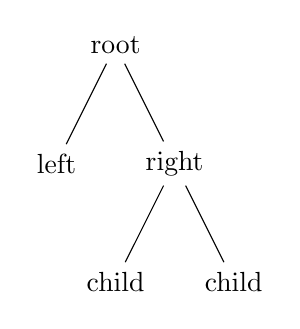
\begin{tikzpicture}
  \node {root}
    child {node {left}}
    child {node {right}
      child {node {child}}
      child {node {child}}
    };
\end{tikzpicture}

A simple image is \tikz \fill (0,0) circle(5pt);.
\end{document}
\end{codeexample}

The method works as follows: if the document is typeset normally, the library
searches for replacement images for every picture. Filenames are generated
automatically in the default configuration. In our case, the two file names
will be |main-figure0| and |main-figure1|. If they exist, those images are
simply included and the pictures as such are not processed. If graphics files
do not exist, steps are taken to generate the missing ones. Since (currently)
only one output file can be set, each missing image needs to be generated by a
separate run of \LaTeX\ in which the |\jobname| is set to the desired image
file name. In the default configuration |mode=convert with system call|, these
commands are issued automatically by using the |\write18| method to call system
commands. It is also possible to output every required file name or to generate
a |makefile|; users will need to issue the required commands manually (or with
|make|). The probably most comfortable way is to use the default configuration
with
%
\begin{codeexample}[code only, tikz syntax=false]
pdflatex -shell-escape main
\end{codeexample}
%
\noindent which authorizes |pdflatex| to call itself recursively to generate
the images. When it finishes, all images are generated and the document already
includes them.

From this point on, successive runs of \LaTeX\ will use the final graphics
files, the pictures won't be used anymore.
Section~\ref{section-libs-external-nopgf} contains details about how to submit
such a file to environments where \pgfname\ is not available.

\begin{command}{\tikzexternalize\oarg{optional arguments}}
    This command activates the externalization. It installs commands to replace
    every \tikzname-picture. It needs to be called before |\begin{document}|
    because it may need to install its separate shipout routine.

    The \meta{optional arguments} can be any of the keys described below.

    Note that the generation/modification of auxiliary files like |.aux|,
    |.toc| etc.\ is usually suppressed while a single image is externalized
    (details for |\label| support follow).

    It is also possible to write |\tikzexternalize|\marg{main job name} if the
    argument is delimited by curly braces. This case is mainly for backwards
    compatibility and is no longer necessary. Since it might be useful in rare
    circumstances, it is documented in section~\ref{sec:external:detail}.

    A detailed description about the process of externalization is provided in
    section~\ref{sec:external:detail}.

    \begin{command}{\tikzexternalrealjob}
        After the library is loaded, this macro will \emph{always} contain the
        correct main job's name (in the example above, it is |main|). It is to
        be used instead of |\jobname| when the externalization is in effect.
    \end{command}
    %
    \begin{command}{\pgfactualjobname}
        Once |\tikzexternalize| has been called, |\pgfactualjobname| contains
        the name of the currently generated output file (which may be |main| or
        |main-figure0| or |main-figure1| in our example above).
    \end{command}
    %
    \begin{command}{\jobname}
        The value of |\jobname| is one of |\tikzexternalrealjob| or
        |\pgfactualjobname|, depending on the configuration. In short: if
        auxiliary file support (|\label| and |\ref|) is activated,
        |\jobname=\tikzexternalrealjob| (since that's the base file name of
        auxiliary files).
    \end{command}
\end{command}

\begin{key}{/tikz/external/system call=\marg{template}}
\label{extlib:systemcall:option}
    A template string used to generate system calls. Inside of \marg{template},
    the macro |\image| can be used as placeholder for the image which is about
    to be generated while |\texsource| contains the main file name (in truth,
    it contains |\input|\marg{main file name}, but that doesn't matter).

    The default depends on the value of |\pgfsysdriver|. For
    |pgfsys-pdftex.def|, it is
    %
\begin{codeexample}[code only]
\tikzset{external/system call={pdflatex \tikzexternalcheckshellescape -halt-on-error
    -interaction=batchmode -jobname "\image" "\texsource"}}
\end{codeexample}
    %
    \noindent where \declareandlabel{\tikzexternalcheckshellescape} inserts the
    value of the configuration key |shell escape| if and only if the current
    document has been typeset with |-shell-escape|\footnote{Note that this is
    always true for the default configuration. This security consideration
    applies mainly for \texttt{mode=list and make} which will also work
    \emph{without} shell escapes.}.

    Other drivers result in slightly different calls. There is support for
    |lualatex|, |xelatex|, and |dvips|. The precise values are written to the
    |.log| file as soon as you attempt to compile a document.

    The argument \marg{template} will be expanded using |\edef|, so any control
    sequences will be expanded. During this evaluation, `|\\|' will result in a
    normal backslash, `|\|'. Furthermore, double quotes `|"|', single quotes
    `|'|', semicolons and dashes `|-|' will be made to normal characters if any
    package uses them as macros. This ensures compatibility with the |german|
    package, for example.
\end{key}

\begin{key}{/tikz/external/shell escape=\marg{command-line arg} (initially -shell-escape)}
    Contains the command line option for |latex| which enables the |\write18|
    feature. For \TeX-Live, this is |-shell-escape|. For MiK\TeX, you should
    use |\tikzexternalize[shell escape=-enable-write18]|.
\end{key}


\subsubsection{Support for Labels and References In External Files}

The |external| library comes with extra support for |\label| and |\ref| (and
other commands which usually store information in the |.aux| file) inside an
external files.

In particular, it supports the two use-cases
%
\begin{enumerate}
    \item[a)] |\ref| to something in the main document inside an externalized
        graphics or
    \item[b)] |\label| in the externalized graphics which is referenced in the
        main document.
\end{enumerate}

The only restriction is that you need to compile your document multiple times
(as usual for references).

\paragraph{NOTE:}
support for a) is unavailable for versions up to and including \pgfname\ 3.0.1.

\begin{key}{/tikz/external/aux in dpth=\marg{boolean} (initially true)}
    Allows to enable or disable the feature which handles references and labels
    as part of image externalization. Disabling it will safe one |\newwrite|
    command, i.e.\ a write register.

    Also see the |disable dependency files| feature.

    Here are some implementation details on how references within/from external
    graphics work for those who would like to know the details:

    For point a), a |\ref| inside of an externalized graphics works by reading
    the main document's |.aux| file. To this end, the standard
    |mode=convert with system call| detects such references and reschedules the
    externalization to |\end{document}.|\footnote{Note that this requires the
    \texttt{atveryend} package. The purpose to reschedule the externalization
    is to access the main job's aux file, but only after it has been written
    completely.} Other values of |mode| require just one attempt to externalize
    the picture.

    Note that |\pageref| is not supported (sorry).

    Point b) works as follows: a |\label| inside of an externalized graphics
    causes the |external| library to generate separate auxiliary files for every
    external image. These files are called \meta{imagename}|.dpth|. The
    extension |.dpth| indicates that the file also contains the image's depth
    (the |baseline| key of \tikzname). Furthermore, anything which would have
    been written to an |.aux| file will be redirected to the |.dpth| file --
    but only things which occur inside of the externalized |tikzpicture|
    environment. When the main document loads the image, it will copy the
    |.dpth| file into the main |.aux| file. Then, successive compilations of
    the main document contain the external |\label| information. In other
    words, a |\label| in an external graphics needs the following work flow:
    %
    \begin{enumerate}
        \item The external graphics needs to be generated together with its
            |.dpth| (usually automatically by \tikzname).
        \item The main document includes the external graphics and copies the
            |.dpth| content into its main |.aux| file.
        \item The main document needs to be translated once again to re-read
            its |.aux| file\footnote{Note that it is not possible to activate
            the content of an auxiliary file after \texttt{\textbackslash
            begin\{document\}} in \LaTeX.}.
    \end{enumerate}

    This does also work if a |\label|/|\ref| combination is implemented itsself
    by a |tikzpicture| (a feature offered by |pgfplots|).
\end{key}


\subsubsection{Customizing the Generated File Names}

The default filename for externalized graphics is `\meta{real file
name}|-figure_|\meta{number}' where \meta{number} ranges from $0$ to whatever
is required. However, there are a couple of ways to change the generated
filenames:
%
\begin{itemize}
    \item Changing the overall file name using a |prefix|,
    \item Changing the file name for a single figure using
        |\tikzsetnextfilename|,
    \item Changing the file name for a restricted set of figures using
        |figure name|.
\end{itemize}

\begin{key}{/tikz/external/prefix=\marg{file name prefix} (initially empty)}
    A shortcut for |\tikzsetexternalprefix|\marg{file name prefix}, see below.
\end{key}

\begin{command}{\tikzsetexternalprefix\marg{file name prefix}}
    Assigns a common prefix used by all file names. For example,
    %
\begin{codeexample}[code only]
\tikzsetexternalprefix{figures/}
\end{codeexample}
    %
    will prepend |figures/| to every external graphics file name.

    Please note that |\tikzsetexternalprefix| is the \emph{only} way to assign
    a prefix in case you want to prepare your document for environments where
    \pgfname\ is not installed (see section~\ref{section-libs-external-nopgf}).
\end{command}

\begin{command}{\tikzsetnextfilename\marg{file name}}
    Sets the file name for the \emph{next} \tikzname\ picture or |\tikz| short
    command. It will \emph{only} be used for the next picture.

    Pictures for which no explicit file name has been set (or the next file
    name is empty) will get automatically generated file names.

    Please note that |prefix| will still be prepended to \marg{file name}.
    %
\begin{codeexample}[code only]
\documentclass{article}
% main document, called main.tex
\usepackage{tikz}

\usetikzlibrary{external}
\tikzexternalize[prefix=figures/] % activate

\begin{document}

\tikzsetnextfilename{trees}
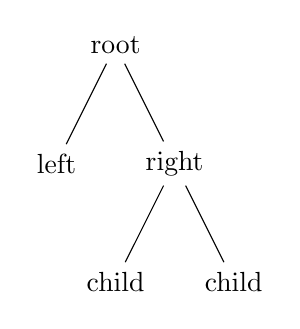
\begin{tikzpicture} % will be written to 'figures/trees.pdf'
  \node {root}
    child {node {left}}
    child {node {right}
      child {node {child}}
      child {node {child}}
    };
\end{tikzpicture}

\tikzsetnextfilename{simple}
A simple image is \tikz \fill (0,0) circle(5pt);. % will be written to 'figures/simple.pdf'


\begin{tikzpicture} % will be written to 'figures/main-figure0.pdf'
   \draw[help lines] (0,0) grid (5,5);
\end{tikzpicture}
\end{document}
\end{codeexample}
    %
\begin{codeexample}[code only, tikz syntax=false]
pdflatex -shell-escape main
\end{codeexample}
    %
\end{command}

\begin{key}{/tikz/external/figure name=\marg{name}}
    Same as |\tikzsetfigurename|\marg{name}.
\end{key}

\begin{command}{\tikzsetfigurename\marg{name}}
    Changes the names of \emph{all} following figures. It is possible to change
    |figure name| during the document either using
    |\tikzset{external/figure name|=\marg{name}|}| or with this command. A
    unique counter will be used for each different \marg{name}, and each
    counter will start at $0$.

    The value of |prefix| will be applied after |figure name| has been
    evaluated.
    %
\begin{codeexample}[code only]
\documentclass{article}
% main document, called main.tex
\usepackage{tikz}

\usetikzlibrary{external}
\tikzexternalize % activate

\begin{document}

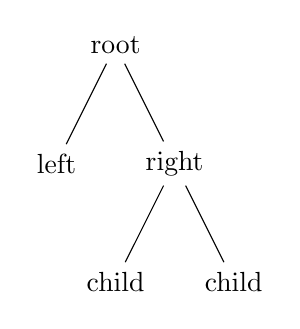
\begin{tikzpicture} % will be written to 'main-figure0.pdf'
  \node {root}
    child {node {left}}
    child {node {right}
      child {node {child}}
      child {node {child}}
    };
\end{tikzpicture}

{
  \tikzsetfigurename{subset_}
  A simple image is \tikz \fill (0,0) circle(5pt);. % will be written to 'subset_0.pdf'

  
\begin{tikzpicture} % will be written to 'subset_1.pdf'
     \draw[help lines] (0,0) grid (5,5);
  \end{tikzpicture}
}% here, the old file name will be restored:

\begin{tikzpicture} % will be written to 'main-figure1.pdf'
   \draw (0,0) -- (5,5);
\end{tikzpicture}
\end{document}
\end{codeexample}
    %
    The scope of |figure name| ends with the next closing brace.

    Remark: Use |\tikzset{external/figure name/.add={prefix_}{_suffix_}}| to
    add a |prefix_| and a |_suffix_| to the actual value of |figure name|.
\end{command}

\begin{command}{\tikzappendtofigurename\marg{suffix}}
    Appends \meta{suffix} to the actual value of |figure name|.

    It is a shortcut for |\tikzset{external/figure name/.add={}|\marg{suffix}|}|
    (a shortcut which is also supported if \tikzname\ is not installed, see
    below).
\end{command}


\subsubsection{Remaking Figures or Skipping Figures}

\begin{command}{\tikzpicturedependsonfile\marg{file name}}
    Adds a dependency for the \emph{next} picture which is about to be
    externalized. If the command is invoked within a picture environment, it
    adds a dependency for the surrounding picture. Dependencies are written
    into \meta{target file}|.dep| in the format

    \meta{target file}|.\tikzexternalimgextension: |\meta{file name}.

    The effect is that if \meta{file name} changes, the external graphics
    associated with the picture shall be remade.

    This command uses the contents of
    \declareandlabel{\tikzexternalimgextension} to check for graphics. If you
    encounter difficulties with image extensions, consider redefining this
    macro (after |\tikzexternalize|).

    \paragraph{Limitations:}
    this command is currently only supported for |mode=list and make| and the
    generated |makefile|.
\end{command}

\begin{command}{\tikzexternalfiledependsonfile\marg{external graphics}\marg{file name}}
    A variant of |\tikzpicturedependsonfile| which adds a dependency for an
    \meta{external graphics}. The argument \meta{external graphics} must be the
    path as it would have been generated by the |external| library, i.e.\ without
    file extension but including any prefixes.
\end{command}

\begin{key}{/tikz/external/disable dependency files}
    Allows to (irreversibly) disable the generation of file dependencies.
    Disabling it will safe one |\newwrite| command, i.e.\ a write register.
    Note that the write register is only allocated if the feature has been used
    at all. This key needs to be provided as argument to |\tikzexternalize| (or
    it needs to be set before calling |\tikzexternalize|).

    Also see the |aux in dpth| key.
\end{key}

\begin{key}{/tikz/external/force remake=\marg{boolean} (default true)}
    A boolean which is used to customize the up-to-date checks of all following
    figures. Every up-to-date check will fail, resulting in automatic
    regeneration of every following figure.
    %
\begin{codeexample}[code only]
\tikzset{external/force remake}

\begin{tikzpicture}
    \draw (0,0) circle(5pt);
\end{tikzpicture}
\end{codeexample}
    %
    You can also use |force remake| inside of a local \TeX\ group to remake
    only selected pictures. The example
    %
\begin{codeexample}[code only]
\tikz \draw (0,0) -- (1,1);

{
\tikzset{external/force remake}

\begin{tikzpicture}
   \draw (0,0) circle(5pt);
\end{tikzpicture}
}

\tikz \draw (0,0) -- (1,1);
\end{codeexample}
    will only apply |force remake| to the second figure.

    Up-to-date checks are applied for |mode=convert with system call| and the
    makefile generated by |mode=list and make|.
\end{key}

\begin{key}{/tikz/external/remake next=\marg{boolean} (default true)}
    A variant of |force remake| which applies only to the next image.
\end{key}

\begin{key}{/tikz/external/export next=\marg{boolean} (default true)}
    A boolean which can be used to disable the export mechanism for single pictures.
\end{key}

\begin{key}{/tikz/external/export=\marg{boolean} (initially true)}
    A boolean which can be used to disable the export mechanism for all
    pictures inside of the current \TeX-scope.
    %
\begin{codeexample}[code only]
\begin{document}
\begin{tikzpicture} % will be exported
    ...
\end{tikzpicture}

{
\tikzset{external/export=false}
\begin{tikzpicture} % won't be exported
    ...
\end{tikzpicture}
...
}

\begin{tikzpicture} % will be exported
    ...
\end{tikzpicture}
\end{document}
\end{codeexample}
    %
    For \LaTeX, the feature lasts until the next |\end|\marg{$\cdot$} (this
    holds for every call to |\tikzset|).
\end{key}

\begin{key}{/tikz/external/up to date check=\marg{choice} (initially md5)}
    The |external| lib has to decide when some existing figure is up-to-date.
    In such a case, it can be used without remaking it. Outdated pictures will
    be remade.

    The key |up to date check| allows to choose among a couple of heuristics
    which are supposed to catch the most important reasons to remake a figure.

    The |up to date check| can be overrule by any of the |force remake| or
    |remake next| keys: if one of them is true, the figure is not up-to-date.

    The choice \declare{simple} is based on the existence of the file: the file
    is up-to-date if and only if it exists.

    The choice \declare{md5} generates an MD5 checksum of the picture for which
    the up-to-date check is running. The MD5 is compared against the MD5 of the
    previous run, which, in turn, will be written into an extra file with the
    extension |.md5|. This file will be modified if and only if the MD5
    comparison indicates a difference. The MD5 computation is based on the
    pdf\TeX\ method |\pdfmdfivesum|. If it is unavailable for some reason, the
    choice |diff| will be used instead.

    The choice \declare{diff} is the same as MD5 -- except that it compares the
    picture content as-is instead of a hash. The |.md5| file will be used to
    compare an old version with the current one -- but its content is some
    ``normalized'' version of the picture for internal use.

    \paragraph{Attention:}
    the content--based strategies |md5| and |diff| operate on the picture
    content -- and only on the picture content. Here, ``picture content'' only
    includes the top--level tokens; no expansion is applied and no included
    files are part of the strategies. If you change preamble styles, you have
    to rebuild the figures manually (for example by deleting the generated
    graphics files). If you have include files, consider using
    |\tikzpicturedependsonfile| and its variants. Since this key provides
    heuristics, you should always remake your figures before you finally
    publish your document. Example: Suppose we have the following picture which
    depends on a command |\mycommand|:
    %
\begin{codeexample}[code only]
\def\mycommand{My comment}

\begin{tikzpicture}

\node at (0,0) {\mycommand};

\end{tikzpicture}
\end{codeexample}
    %
    What happens if you change ``My comment'' to ``My super comment''? Well,
    |external| will \emph{not} pick it up; you will need to handle this
    manually. However, if you modify anything between |\begin{tikzpicture}| and
    |\end{tikzpicture}|, the |external| library \emph{will} pick it up and
    regenerate the picture.

    The |up to date check| is applied for |mode=convert with system call| and
    |mode=list and make|.
\end{key}

\begin{command}{\tikzexternaldisable}
    Allows to disable the complete externalization. While |export next| will
    still collect the contents of picture environments, this command uninstalls
    the hooks for the |external| library completely. Thus, nested picture
    environments or environments where |\end{tikzpicture}| is not directly
    reachable won't produce compilation failures -- although it is not possible
    to externalize them automatically.

    The externalization remains disabled until the end of the next \TeX\ group
    (or environment) or until the next call to |\tikzexternalenable|.
\end{command}

\begin{command}{\tikzexternalenable}
    Re-enables a previously running externalization after |\tikzexternaldisable|.
\end{command}


\subsubsection{Customizing the Externalization}

\begin{key}{/tikz/external/figure list=\marg{boolean} (initially true)}
    A boolean which configures whether a figure list shall be generated. A
    figure list is an output file named \marg{jobname}|.figlist| which is
    filled with file names of each figure, one per line.

    This file is not used by \TeX\ anymore, its purpose is to issue the
    required conversion commands |pdflatex -jobname |\marg{picture file name}
    \marg{main file} manually (or in a script). See
    section~\ref{sec:external:detail} for the details about the expected system
    call (or activate |mode=convert with system call| and inspect your log
    file).
    %
\begin{codeexample}[code only]
\documentclass{article}
% main document, called main.tex
\usepackage{tikz}

\usetikzlibrary{external}
\tikzexternalize[
   mode=graphics if exists,
   figure list=true,
   prefix=figures/]

\begin{document}

\tikzsetnextfilename{trees}
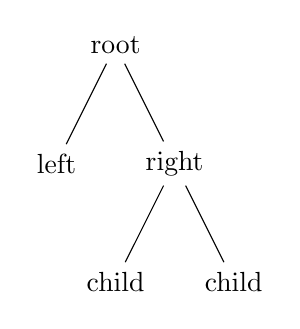
\begin{tikzpicture}
  \node {root}
    child {node {left}}
    child {node {right}
      child {node {child}}
      child {node {child}}
    };
\end{tikzpicture}

\tikzsetnextfilename{simple}
A simple image is \tikz \fill (0,0) circle(5pt);.


\begin{tikzpicture}
   \draw[help lines] (0,0) grid (5,5);
\end{tikzpicture}
\end{document}
\end{codeexample}

\begin{codeexample}[code only, tikz syntax=false]
pdflatex main
\end{codeexample}
    %
    generates |main.figlist| containing
    %
\begin{codeexample}[code only, tikz syntax=false]
figures/trees
figures/simple
figures/main-figure0
\end{codeexample}
    %
\end{key}

\begin{key}{/tikz/external/mode=\marg{choice} (initially convert with system call)}
    Configures what to do with \tikzname\ pictures (unless we are currently
    externalizing one particular image, in that case, these modes are ignored).

    The preconfigured mode |convert with system call| checks whether external
    graphics files are up-to-date and includes them if that is the case. Any
    picture which is not up-to-date will be generated automatically using a
    system call. The system call can be configured using the |system call|
    template. The up-to-date check is applied according to the
    |up to date check| key. As soon as |convert with system call| is set, the
    |figure list| will be disabled -- such a file is not required. In case you
    still need or want it, you can enable it after setting |mode|.

    Please note that system calls may be disabled for security reasons. For
    pdflatex, they can be enabled using
    %
\begin{codeexample}[code only, tikz syntax=false]
pdflatex -shell-escape
\end{codeexample}
    %
    while other \TeX\ variants may need other switches. The feature is
    sometimes called |\write18|.

    The choice |only graphics| always tries to replace pictures with external
    graphics. It is an error if the graphics file does not exist.

    The choice |no graphics| (or, equivalently, |only pictures|) typesets
    \tikzname\ pictures without checking for external graphics.

    A mixture is |graphics if exists|, it checks whether a suitable graphics
    file exists and includes it if that is the case. If it does not exist, the
    picture is typeset using \TeX.

    Mode |list only| skips every \tikzname\ picture; it only generates the file
    \marg{main file}|.figlist| containing file names for every picture, the
    contents of any picture environment is thrown away and a replacement text
    is shown. This implies |figure list=true|. See also the |list and make|
    mode which includes available graphics.

    The mode |list and make| is similar to |list only|: it generates the same
    file \marg{main file}|.figlist|, but any images which exist already are
    included as graphics instead of ignoring them. Furthermore, this mode
    generates an additional file: \marg{main file}.makefile. This allows to use
    a work flow like
    %
\begin{codeexample}[code only, tikz syntax=false]
% step 1: generate main.makefile:
pdflatex main
% step 2: generate ALL graphics on 2 processors:
make -j 2 -f main.makefile
% step 3: include the graphics:
pdflatex main
\end{codeexample}
    %
    \noindent This last make method is optional: |list and make| just assumes
    that images are generated somehow (not necessarily with the generated
    makefile). The generated makefile allows parallel externalization of
    graphics on multi-core systems and it supports any file dependencies
    configured with |\tikzpicturedependsonfile|. Furthermore, it respects the
    |force remake| and |remake next| keys.
\end{key}

\begin{key}{/tikz/external/verbose IO=\marg{boolean} (initially true)}
    A boolean which configures whether I/O operations shall be listed in the
    logfile.
\end{key}

\begin{key}{/tikz/external/verbose optimize=\marg{boolean} (initially true)}
    A boolean which configures whether optimization operations shall be listed
    in the logfile.
\end{key}

\begin{key}{/tikz/external/verbose=\marg{boolean} (initially true)}
    Sets all verbosity flags to \meta{boolean}.
\end{key}

\begin{key}{/tikz/external/optimize=\marg{boolean} (initially true)}
    Configures whether the conversion process shall be optimized. This affects
    only the case when |\jobname| differs from the main file name, i.e.\ when
    single pictures are converted.

    In that case, the main file is compiled as usual -- but everything except
    the selected picture is thrown away. If optimization is enabled, all other
    pictures won't be processed at all. Furthermore, expensive commands which
    do not contribute to the selected picture will be thrown away as well.

    The default implementation discards |\includegraphics| commands which are
    \emph{not} inside of the selected picture to reduce conversion time.

    It is possible to add commands which shall be optimized away, see below.
\end{key}

\begin{key}{/tikz/external/optimize command away=\meta{\textbackslash command}\marg{required argument count}}
    Installs commands to optimize \meta{\textbackslash command} away. As is
    described above, optimization applies to the case when single pictures are
    converted: one usually doesn't need to process (probably expensive)
    commands which do not contribute to the selected picture.

    The argument \marg{required argument count} is either empty or a
    non-negative integer between $0$ and $9$. It denotes the number of
    arguments which should be consumed after \meta{\textbackslash command}. In
    any case, one argument in square brackets after the command will be
    recognized as well. To be more precise, the following cases for arguments
    of \meta{\textbackslash command} are supported:
    %
    \begin{enumerate}
        \item If \marg{required argument count} is empty (the default),
            \meta{\textbackslash command} may take one optional argument in
            square brackets and one in curly braces (which is also optional).
        \item If \marg{required argument count} is not empty,
            \marg{\textbackslash command} may take one optional argument in
            square brackets. Furthermore, it expects exactly \marg{required
            argument count} following arguments.
    \end{enumerate}

    Example:
    %
\begin{codeexample}[code only]
\tikzset{external/optimize command away=\includegraphics}
\end{codeexample}

\begin{codeexample}[code only]
\newcommand{\myExpensiveMacro}[1]{Very expensive!}

\tikzset{external/optimize command away=\myExpensiveMacro}
\end{codeexample}

\begin{codeexample}[code only]
\newcommand{\myExpensiveMacroWithThreeArgs}[3]{Very expensive!}

\tikzset{external/optimize command away={\myExpensiveMacroWithThreeArgs}{3}}
\end{codeexample}

\begin{codeexample}[code only]
% A command with optional argument:
\newcommand{\aFurtherExample}[3][]{Very expensive!}

% consume only two arguments: the first optional one will be processed
% anyway:
\tikzset{external/optimize command away={\myExpensiveMacroWithThreeArgs}{2}}
\end{codeexample}
    %
    The argument \meta{\textbackslash command} must be the name of a single
    macro. Any occurrence of this macro, together with its arguments, will be
    removed.
    %
\begin{codeexample}[code only]
\begin{tikzpicture}
    % this picture is currently converted!
\end{tikzpicture}

This here is outside of the converted picture and contains \myExpensiveMacro. It will be discarded.

This call: \myExpensiveMacro[argument=value]{Argument} as well.
And this here: \myExpensiveMacro{Argument} also.
\end{codeexample}

    The default is to optimize |\includegraphics| away.

    This key is actually a style which sets the |optimize/install| and
    |optimize/restore| keys.
\end{key}

\begin{key}{/tikz/external/optimize/install}
    A command key which contains code to install optimizations. You can append
    code here (or clear the macro) if you need to modify the optimization.
\end{key}

\begin{key}{/tikz/external/optimize/restore}
    A command key which contains code to undo optimizations. You can append
    code here (or clear the macro) if you need to modify the optimization.
\end{key}

\begin{key}{/tikz/external/only named=\marg{boolean} (initially false)}
    If enabled, only pictures for which file names have been set explicitly
    using |\tikzsetnextfilename| will be considered, no file names will be
    generated automatically.
\end{key}

\begin{key}{/pgf/images/include external (initially \textbackslash pgfimage\{\#1\})}
\index{External Graphics!Bounding Box Issues}
    This command key constitutes the public interface to exchange the
    |\includegraphics| command used for the image inclusion. If can be
    overwritten using |include external/.code=|\marg{\TeX\ code}.

    Its description can be found in the corresponding basic layer documentation
    on page~\pageref{pgf:includeexternalkey}.

    Just one example here: you can use
    %
\begin{codeexample}[code only]
\pgfkeys{/pgf/images/include external/.code={\includegraphics[viewport=0 0 211.28 175.686]{#1}}}
\end{codeexample}
    %
    to manually change the viewport (bounding box) for included graphics.

    Another example (of probably limited use) is
    %
\begin{codeexample}[code only]
\pgfkeys{/pgf/images/include external/.code={\href{file:#1}{\pgfimage{#1}}}}
\end{codeexample}
    %
    \noindent which will generate a clickable hyperlink around the image.
    Clicking on it opens the single exported file\footnote{This requires all
    external graphics files in the same base directory as the main |.pdf|
    file.}.

    If you want to limit the effects of this key to just one externalized
    figure, use
    %
\begin{codeexample}[code only]
{
  \pgfkeys{/pgf/images/include external/.code={\includegraphics[viewport=0 0 211.28 175.686]{#1}}}
  \begin{tikzpicture}
     ...
  \end{tikzpicture}
}% this brace ends the effect of `include external'
\end{codeexample}
    %
\end{key}

\begin{command}{\tikzifexternalizing\marg{true code}\marg{false code}}
    This command can be used to check whether an image is currently written to
    its separate graphics file (if the ``grab'' procedure is running). If so,
    the \marg{true code} will be executed. If not, that means if the main
    document is being typeset normally, the \marg{false code} will be invoked.

    This command must be used \emph{after} |\tikzexternalize|.
\end{command}

\begin{command}{\tikzifexternalizingnext\marg{true code}\marg{false code}}
    Like |\tikzifexternalizing|, but this variant also checks if the next
    following figure is the one which is about to be written to its separate
    graphics file.
\end{command}


\subsubsection{Details About The Process}
\label{sec:external:detail}

The standard run |pdflatex |\meta{main document} causes the |external| library
to check every occurrence of |\begin{tikzpicture}| and every |\tikz| short
command. If it finds a picture which shall be exported, it queries the
respective file name and checks whether the file exists already. If so, it
includes the external graphics. If not, it requires an externalization which
can be done automatically (the default), semi-automatically (with
|mode=list and make|) or manually (by issuing the requires system calls
somehow).

The library can detect whether it runs in ``conversion mode'', i.e.\ if it
should only process a single image. To do so, it checks whether the internal
macro \declareandlabel{\tikzexternalrealjob} exists. If so, its contents is
assumed to be \meta{main document} (without the suffix |.tex|). Usually, this
macro is set by the conversion system call,
%
\begin{codeexample}[code only, tikz syntax=false]
pdflatex -jobname "main-figure0" "\def\tikzexternalrealjob{main}%%% File encoding: UTF-8
%%% äöüÄÖÜß  <-- keine deutschen Umlaute hier? UTF-faehigen Editor verwenden!

%%% Magic Comments zum Setzen der korrekten Parameter in kompatiblen IDEs
% !TeX encoding = utf8
% !TeX program = pdflatex 
% !TeX spellcheck = de_DE
% !BIB program = biber

\documentclass[master,german,smartquotes]{hgbthesis}
% Zulässige Optionen in [..]: 
%   Typ der Arbeit: diploma, master (default), bachelor, internship 
%   Hauptsprache: german (default), english
%		smartquotes: 
%%%----------------------------------------------------------

\RequirePackage[utf8]{inputenc}		% bei der Verw. von lualatex oder xelatex entfernen!

\graphicspath{{images/}}    % Verzeichnis mit Bildern und Grafiken
\logofile{logo}				% Logo-Datei = images/logo.pdf (\logofile{}, wenn kein Logo gewünscht)
\bibliography{references}  	% Biblatex-Literaturdatei (references.bib)

%%%----------------------------------------------------------
% Angaben für die Titelei (Titelseite, Erklärung etc.)
%%%----------------------------------------------------------

%%% Einträge für ALLE Arbeiten: -----------------------------
\title{Partielle Lösungen zur allgemeinen Problematik}
\author{Peter A.\ Schlaumeier}
\programname{Universal Computing}
\placeofstudy{Hagenberg}
\dateofsubmission{2019}{07}{15}	% {YYYY}{MM}{DD}

%%% Zusätzlich für eine Bachelorarbeit: ---------------------
\thesisnumber{XXXXXXXXXX-A}   % Stud-ID, z.B. 1310238045-A  
% (A = 1. Bachelorarbeit)
\semester{Sommersemester 2017} 
\coursetitle{Einführung in die Tiefere Problematik 1} 
\advisor{Alois B.~Treuer, Päd.\ Phil.}

%%% Restriktive Lizenformel anstatt CC (nur für Typ master) -
%\strictlicense

%%%----------------------------------------------------------
\begin{document}
%%%----------------------------------------------------------

%%%----------------------------------------------------------
\frontmatter                    % Titelei (röm. Seitenzahlen)
%%%----------------------------------------------------------

\maketitle
\tableofcontents

\chapter{Vorwort} 	% engl. Preface


Dies ist \textbf{Version \hgbDate} der \latex-Dokumentenvorlage für 
verschiedene Abschlussarbeiten an der Fakultät für Informatik, Kommunikation
und Medien der FH Oberösterreich in Hagenberg, die mittlerweile auch 
an anderen Hochschulen im In- und Ausland gerne verwendet wird.

Das Dokument entstand ursprünglich auf Anfragen von Studierenden,
nachdem im Studienjahr 2000/01 erstmals ein offizieller
\latex-Grundkurs im Studiengang Medientechnik und -design an der
FH Hagenberg angeboten wurde. Eigentlich war die Idee, die bereits
bestehende \emph{Word}-Vorlage für Diplomarbeiten "einfach" in
\latex\ zu übersetzen und dazu eventuell einige spezielle
Ergänzungen einzubauen. Das erwies sich rasch als wenig
zielführend, da \latex, \va was den Umgang mit Literatur und
Grafiken anbelangt, doch eine wesentlich andere Arbeitsweise
verlangt. Das Ergebnis ist -- von Grund auf neu geschrieben und
wesentlich umfangreicher als das vorherige Dokument --
letztendlich eine Anleitung für das Schreiben mit \latex, ergänzt
mit einigen speziellen (mittlerweile entfernten) Hinweisen für \emph{Word}-Benutzer.
Technische Details zur aktuellen Version finden sich in Anhang \ref{app:TechnischeInfos}.

Während dieses Dokument anfangs ausschließlich für die Erstellung
von Diplomarbeiten gedacht war, sind nunmehr auch  
\emph{Masterarbeiten}, \emph{Bachelor\-arbeiten} und \emph{Praktikumsberichte} 
abgedeckt, wobei die Unterschiede bewusst gering gehalten wurden.

Bei der Zusammenstellung dieser Vorlage wurde versucht, mit der
Basisfunktionalität von \latex das Auslangen zu finden und -- soweit möglich --
auf zusätzliche Pakete zu verzichten. Das ist nur zum Teil gelungen;
tat\-säch\-lich ist eine Reihe von ergänzenden "Paketen" notwendig, wobei jedoch
nur auf gängige Erweiterungen zurückgegriffen wurde.
Selbstverständlich gibt es darüber hinaus eine Vielzahl weiterer Pakete,
die für weitere Verbesserungen und Finessen nützlich sein können. Damit kann
sich aber jeder selbst beschäftigen, sobald das notwendige Selbstvertrauen und
genügend Zeit zum Experimentieren vorhanden sind.
Eine Vielzahl von Details und Tricks sind zwar in diesem Dokument nicht explizit
angeführt, können aber im zugehörigen Quelltext jederzeit ausgeforscht
werden.

Zahlreiche KollegInnen haben durch sorgfältiges Korrekturlesen und
konstruktive Verbesserungsvorschläge wertvolle Unterstützung
geliefert. Speziell bedanken möchte ich mich bei Heinz Dobler für
die konsequente Verbesserung meines "Computer Slangs", bei
Elisabeth Mitterbauer für das bewährte orthographische Auge und
bei Wolfgang Hochleitner für die Tests unter Mac~OS.

Die Verwendung dieser Vorlage ist jedermann freigestellt und an
keinerlei Erwähnung gebunden. Allerdings -- wer sie als Grundlage
seiner eigenen Arbeit verwenden möchte, sollte nicht einfach
("ung'schaut") darauf los werken, sondern zumindest die
wichtigsten Teile des Dokuments \emph{lesen} und nach Möglichkeit
auch beherzigen. Die Erfahrung zeigt, dass dies die Qualität der
Ergebnisse deutlich zu steigern vermag.

Dieses Dokument und die zugehörigen \latex-Klassen sind seit Nov.\ 2017 auf CTAN%
\footnote{Comprehensive TeX Archive Network} 
als Paket \texttt{hagenberg-thesis} verfügbar unter
%
\begin{itemize}
\item[]\url{https://ctan.org/pkg/hagenberg-thesis}.
\end{itemize}
%
Den jeweils aktuellen Quelltexte sowie zusätzliche Materialien findet man unter
%
\begin{itemize}
\item[]\url{https://github.com/Digital-Media/HagenbergThesis}.%
\footnote{Unter \url{https://github.com/Digital-Media/HagenbergThesis/blob/master/CHANGELOG.md}
sowie genauer unter \url{https://github.com/Digital-Media/HagenbergThesis/commits/master} 
findet man auch eine (früher im Anhang dieses Dokuments enthaltene) chronologische Auflistung der 
Änderungen.}
\end{itemize}



\noindent
Trotz großer Mühe enthält ein Dokument wie dieses immer Fehler und Unzulänglichkeiten
-- Kommentare, Verbesserungsvorschläge und sinnvolle Ergänzungen
sind daher willkommen, am einfachsten als Kommentar oder Fehlermeldung ("Issue") 
auf GitHub oder jederzeit auch per E-Mail an
%
\begin{itemize}
\item[]
Dr.\ Wilhelm Burger, Department für Digitale Medien,\newline
Fachhochschule Oberösterreich, Campus Hagenberg (Österreich)\newline
\nolinkurl{wilhelm.burger@fh-hagenberg.at}
\end{itemize}

\noindent
Übrigens, hier im Vorwort (das bei Diplom- und Masterarbeiten üblich, bei Bachelorarbeiten 
aber entbehrlich ist) kann kurz auf die Entstehung des Dokuments eingegangen werden.
Hier ist auch der Platz für allfällige Danksagungen (\zB an den Betreuer, 
den Begutachter, die Familie, den Hund, \ldots), Widmungen und philosophische 
Anmerkungen. Das sollte man allerdings auch nicht übertreiben und auf 
einen Umfang von maximal zwei Seiten beschränken.




 % Optional. Ggf. weglassen
\chapter{Kurzfassung}

\begin{german}
An dieser Stelle steht eine Zusammenfassung der Arbeit, Umfang
max.\ 1 Seite. 
...
\end{german}		
This document gives a quick, relatively minimal example of the use of
\texttt{uafthesis.cls}, while trying to show its features.

This section is contained in \texttt{abstract.tex}.
			

%%%----------------------------------------------------------
\mainmatter          % Hauptteil (ab hier arab. Seitenzahlen)
%%%----------------------------------------------------------

\chapter{Einleitung}
\label{cha:Einleitung}

\section{Zielsetzung}
Dieses Dokument ist als vorwiegend technische Starthilfe für das
Erstellen einer Masterarbeit (oder Bachelorarbeit) mit \latex
gedacht und ist die Weiterentwicklung einer früheren
Vorlage\footnote{Nicht mehr verfügbar.} für das Arbeiten mit
Microsoft \emph{Word}. Während ursprünglich daran gedacht war, die
bestehende Vorlage einfach in \latex zu übernehmen, wurde rasch
klar, dass allein aufgrund der großen Unterschiede zum Arbeiten
mit \emph{Word} ein gänzlich anderer Ansatz notwendig wurde. Dazu
kamen zahlreiche Erfahrungen mit Diplomarbeiten in den
nachfolgenden Jahren, die zu einigen zusätzlichen Hinweisen Anlass gaben.

Das vorliegende Dokument dient einem zweifachen Zweck: 
\emph{erstens} als Erläuterung und Anleitung, \emph{zweitens} als
direkter Ausgangspunkt für die eigene Arbeit. Angenommen wird,
dass der Leser bereits über elementare Kenntnisse im Umgang mit
\latex verfügt. In diesem Fall sollte -- eine einwandfreie
Installation der Software vorausgesetzt -- der Arbeit nichts mehr
im Wege stehen. Auch sonst ist der Start mit \latex\ nicht
schwierig, da viele hilfreiche Informationen auf den zugehörigen
Webseiten zu finden sind (s.\ Kap.~\ref{cha:ArbeitenMitLatex}).





\section{Warum {\latex}?}

Diplomarbeiten, Dissertationen und Bücher im
technisch-natur\-wissen\-schaft\-lichen Bereich werden
traditionell mithilfe des Textverarbeitungssystems \latex
\cite{Lamport1994, Lamport1995} gesetzt. Das hat gute Gründe, denn
\latex ist bzgl.\ der Qualität des Druckbilds, des Umgangs mit
mathematischen Elementen, Literaturverzeichnissen etc.\
unübertroffen und ist noch dazu frei verfügbar. Wer mit \latex
bereits vertraut ist, sollte es auch für die Abschlussarbeit
unbedingt in Betracht ziehen, aber auch für den Anfänger sollte
sich die zusätzliche Mühe am Ende durchaus lohnen.

Für den professionellen elektronischen Buchsatz wurde früher
häufig \emph{Adobe Framemaker} verwendet, allerdings ist diese
Software teuer und komplex. Eine modernere Alternative dazu ist
\emph{Adobe InDesign}, wobei allerdings die Erstellung
mathematischer Elemente und die Verwaltung von Literaturverweisen
zur Zeit nur rudimentär unterstützt werden.%
\footnote{Angeblich werden aber für den (sehr sauberen) Schriftsatz 
in \emph{InDesign} ähnliche Algorithmen wie in \latex\ verwendet.}

Microsoft \emph{Word} gilt im Unterschied zu \latex, 
\emph{Framemaker} und \emph{InDesign} übrigens nicht als professionelle
Textverarbeitungssoftware, obwohl es immer häufiger auch von
großen Verlagen verwendet wird.%
\footnote{Siehe auch \url{http://latex.tugraz.at/mythen.php}.}
Das Schriftbild in \emph{Word}
lässt -- zumindest für das geschulte Auge -- einiges zu wünschen
übrig und das Erstellen von Büchern und ähnlich großen Dokumenten
wird nur unzureichend unterstützt. Allerdings ist \emph{Word} sehr
verbreitet, flexibel und vielen Benutzern zumindest oberflächlich
vertraut, sodass das Erlernen eines speziellen Werkzeugs wie
\latex\ ausschließlich für das Erstellen einer Abschlussarbeit
manchen verständlicherweise zu mühevoll ist. Es sollte daher
niemandem übel genommen werden, wenn er/sie sich auch bei der Abschlussarbeit
auf \emph{Word} verlässt. Im Endeffekt lässt sich mit etwas
Sorgfalt (und ein paar Tricks) auch damit ein durchaus akzeptables
Ergebnis erzielen. 
Ansonsten sollten auch für \emph{Word}-Benutzer 
einige Teile dieses Dokuments von Interesse sein, insbesondere die
Abschnitte über Abbildungen und Tabellen
(Kap.~\ref{cha:Abbildungen}) und mathematische Elemente
(Kap.~\ref{cha:Mathematik}).


\section{Aufbau der Arbeit}

Hier am Ende des Einleitungskapitels (und nicht
etwa in der Kurzfassung) ist der richtige Platz, um die
inhaltliche Gliederung der nachfolgenden Arbeit zu beschreiben.
Hier sollte man darstellen, welche Teile (Kapitel) der Arbeit
welche Funktion haben und wie sie inhaltlich zusammenhängen. Auch
die Inhalte des \emph{Anhangs} -- sofern vorgesehen -- sollten hier
kurz beschrieben werden.

Zunächst sind in Kapitel \ref{cha:Abschlussarbeit} einige wichtige
Punkte zu Abschlussarbeiten im Allgemeinen zusammengefasst.
Kapitel \ref{cha:ArbeitenMitLatex} beschreibt die Idee und die
grundlegenden technischen Eigenschaften von \latex.
Kapitel \ref{cha:Abbildungen} widmet sich der Erstellung von Abbildungen
und Tabellen sowie der Einbindung von Quellcode.
Mathematische Elemente und Gleichungen sind das Thema in Kapitel \ref{cha:Mathematik} 
\usw
Anhang \ref{app:TechnischeInfos} enthält technische Details zu
dieser Vorlage, 
Anhang \ref{app:cdrom} enthält eine Auflistung von zugehörigen Materialien
auf einem beigelegten Speichermedium, und 
Anhang \ref{app:Fragebogen} zeigt ein Beispiel für die
Einbindung eines mehrseitigen PDF-Dokuments.







\chapter{Die Abschlussarbeit}
\label{cha:Abschlussarbeit}

Jede Abschlussarbeit%
\footnote{Die meisten der folgenden Bemerkungen gelten gleichsam für Bachelor-, Master- und Diplomarbeiten.} 
ist anders und dennoch sind sich gute
Arbeiten in ihrer Struktur meist sehr ähnlich, \va\ bei
technisch-natur\-wissen\-schaft\-lichen Themen. 

\section{Elemente der Abschlussarbeit}

Als Ausgangspunkt bewährt hat sich der folgende Grundaufbau, der natürlich 
vari\-iert und beliebig verfeinert werden kann:
%
\begin{enumerate}
\item \textbf{Einführung und Motivation}: Was ist die Problem- oder Aufgabenstellung und
warum sollte sich jemand dafür interessieren?
\item \textbf{Präzisierung des Themas}: Hier wird der aktuelle Stand der Technik
oder Wissenschaft ("State-Of-The-Art") beschrieben, es werden bestehende
Defizite oder offene Fragen aufgezeigt und daraus die
Stoßrichtung der eigenen Arbeit entwickelt.
\item \textbf{Eigener Ansatz}: Das ist natürlich der Kern der Arbeit. Hier
wird gezeigt, wie die vorher beschriebene Aufgabenstellung gelöst und --
häufig in Form eines Programms%
\footnote{\emph{Prototyp} ist in diesem Zusammenhang ein gerne benutzter Begriff, der im Deutschen
allerdings oft unrichtig dekliniert wird. Richtig ist: der \emph{Prototyp}, des \emph{Prototyps}, dem/den \emph{Protototyp} -- falsch hingegen \zB: des \emph{Prototyp\underline{en}}!
} --
realisiert wird, ergänzt durch illustrative Beispiele.
\item \textbf{Zusammenfassung}: Was wurde erreicht und welche Ziele sind
noch offen geblieben, wo könnte weiter gearbeitet werden?
\end{enumerate}
%
Natürlich ist auch ein gewisser dramaturgischer Aufbau der Arbeit
wichtig, wobei zu bedenken ist, dass der Leser in der Regel nur
wenig Zeit hat und -- anders als etwa bei einem Roman -- seine
Geduld nicht auf die lange Folter gespannt werden darf. Erklären
Sie bereits in der Einführung (und nicht erst im letzten Kapitel),
wie Sie an die Sache herangehen, welche Lösungen Sie vorschlagen
und wie erfolgreich Sie damit waren.

Übrigens, auch Fehler und Sackgassen dürfen (und sollten)
beschrieben werden; ihre Kenntnis hilft oft doppelte Experimente und
weitere Fehler zu vermeiden und ist damit sicher nützlicher als
jede Schönfärberei.
Und natürlich ist es auch nicht verboten, seine eigene Meinung 
in sachlicher Form zu äußern.


\section{Arbeiten in Englisch}
\label{sec:englisch}

Diese Vorlage ist zunächst darauf abgestellt, dass die
Abschlussarbeit in deutscher Sprache erstellt wird. Vor allem bei
Arbeiten, die in Zusammenarbeit mit größeren Firmen oder
internationalen Instituten entstehen, ist es häufig erwünscht,
dass die Abschlussarbeit zu besseren Nutzbarkeit in englischer
Sprache verfasst wird, und viele Hochschulen%
\footnote{Die FH Oberösterreich macht hier keine Ausnahme. 
Der Begriff "Fachhochschule" wird dabei entweder gar nicht
übersetzt oder -- wie im deutschsprachigen Raum mittlerweile üblich -- 
mit \emph{University of Applied Sciences}.
%Die offizielle englische Übersetzung von "Medientechnik und -design"
%ist übrigens \emph{Media Technology and Design}.
} 
lassen dies in
der Regel auch zu.

Beachtet sollte allerdings werden, dass das Schreiben dadurch nicht
einfacher wird, auch wenn einem Worte und Sätze im Englischen
scheinbar leichter "aus der Feder" fließen. Gerade im Bereich
der Informatik erscheint durch die Dominanz englischer
Fachausdrücke das Schreiben im Deutschen mühsam und das Ausweichen
ins Englische daher besonders attraktiv. Das ist jedoch
trügerisch, da die eigene Fertigkeit in der Fremdsprache
(trotz der meist langjährigen Schulbildung) häufig überschätzt wird.
Prägnanz und Klarheit gehen leicht verloren und bisweilen ist das
Resultat ein peinliches Gefasel ohne Zusammenhang und soliden
Inhalt. Sofern die eigenen Englischkenntnisse nicht wirklich gut sind, ist
es ratsam, zumindest die wichtigsten Teile der Arbeit zunächst in
Deutsch zu verfassen und erst nachträglich zu übersetzen. Besondere Vorsicht ist bei der Übersetzung von scheinbar
vertrauten Fachausdrücken angebracht. Zusätzlich ist es immer zu
empfehlen, die fertige Arbeit von einem "native speaker"
korrigieren zu lassen.



Technisch ist, außer der Spracheinstellung und den
unterschiedlichen Anführungszeichen (s.\
Abschn.~\ref{sec:anfuehrungszeichen}), für eine englische Arbeit
nicht viel zu ändern, allerdings sollte Folgendes beachtet werden:
%
\begin{itemize}
\item  Die Titelseite (mit der Bezeichnung "Diplomarbeit" oder "Masterarbeit") 
ist für die einzureichenden Exemplare jedenfalls in \emph{deutsch} zu halten,
auch wenn der Titel englisch ist. 
\item Ebenso muss neben dem
englischen \emph{Abstract} auch eine deutsche \emph{Kurzfassung}
enthalten sein. %
\item Akademische Titel von Personen haben im Englischen offenbar
weniger Bedeutung als im Deutschen und werden daher meist
weggelassen.
\end{itemize}

\chapter{Zum Arbeiten mit \latex}
\label{cha:ArbeitenMitLatex}

\section{Einstieg}
\label{sec:LatexEinstieg}

\latex ist eine in den Naturwissenschaften sehr verbreitete
und mittlerweile klassische Textverarbeitungssoftware für das Erstellen
großer und komplizierter Dokumente mit professionellem Anspruch.
Das Arbeiten mit \latex erscheint -- zumindest für den ungeübten Benutzer -- %
zunächst schwieriger als mit herkömmlichen Werkzeugen für die
Textverarbeitung.

Zum Ersten ist -- im Unterschied zu den meisten gängigen
Text\-ver\-arbei\-tungs\-prog\-ram\-men -- \latex nicht \textsc{Wysiwyg}%
\footnote{"What You See Is What You Get." Es gibt auch 
\textsc{Wysiwyg}-Implementierungen für \latex, 
\zB\ \emph{Scientific WorkPlace} (\url{https://www.mackichan.com/}) oder
\emph{LyX} (\url{https://www.lyx.org/}), 
die aber teuer \bzw\ relativ langsam sind.},
sondern es handelt sich um eine \emph{Markup Lang\-uage} (wie HTML) -- noch dazu
eine für den Anfänger recht komplizierte -- und zugehörige Werkzeuge.
Ungewohnt erscheinen sicher auch die vermeintlich starken
Einschränkungen von \latex,
insbesondere in Bezug auf die Wahl der Schriften und das
Layout. Während anfangs of der Eindruck entsteht, dass diese Rigidität
die eigene Kreativität beschränkt, fällt mit der Zeit auf, dass es gerade
dadurch gelingt, sich stärker auf die Inhalte der Arbeit zu
konzentrieren als auf deren äußere Form. Dass am Ende die Form dennoch stimmt,
ist allerdings nur dann gewährleistet, wenn man sich bei den eigenen Modifikationen
der Formate und Parameter äußerste Zurückhaltung auferlegt, es sei denn,
man ist in der Zwischenzeit bereits selbst zum \latex-\emph{Guru} avanciert.

Insgesamt lohnt sich der Aufwand, wie viele meinen, zumal die Abschlussarbeit
in jedem Fall (mit oder ohne \latex) ein substantielles Stück Arbeit ist.
Allerdings sollte mithilfe von \latex ein professionell aussehendes
Ergebnis einfacher zu erreichen sein und es dürfte wohl auch einiger
Ärger mit Fehlern und Einschränkungen gängiger Software erspart bleiben.
Zudem könnte es durchaus sein, dass sich nebenbei auch das eigene Auge für
die Feinheiten des Buchsatzes (weiter-){\obnh}entwickelt.%
\footnote{Dieses abschließende Textelement wurde übrigens zur Ermöglichung eines 
Zeilenumbruchs nach der Klammer so gesetzt: \texttt{\ldots (weiter-)\{{\bs}optbreaknh\}entwickelt.}
Das Makro \texttt{{\bs}optbreaknh} ("optional break with no hyphen") ist in 
\texttt{hgb.sty} definiert.}


\subsection{Software}
\label{sec:Software}

Zum Arbeiten mit \latex wird -- neben einem Computer -- natürlich Software benötigt. Mussten früher oft die einzelnen Komponenten von \latex mühevoll zusammengesucht und für die eigene Umgebung konfiguriert werden, gibt es mittlerweile für die wichtigsten Plattformen (Windows, Mac~Os, Linux) fertige \latex-Installationen, die ohne weiteres Zutun laufen. Die aktuelle Version von \latex\ ist \LaTeXe\ (sprich "LaTeX zwei e"). 
Zum Arbeiten mit \latex\ werden zwei Dinge benötigt:
%
\begin{itemize}
\item \latex-Installation (Distribution),
\item Texteditor oder Autorenumgebung (Frontend).
%\item PostScript/PDF-Software 
\end{itemize}
%
Sämtliche Komponenten sind kostenlos und für alle gängigen Plattformen verfügbar.


\subsubsection{Windows}
\label{sec:Windows}

Unter \emph{Windows} (XP und höher) hat sich folgendes Setup bewährt,
mit dem \ua auch dieses Dokument erstellt wurde:
%
\begin{itemize}
\item \textbf{\latex-Distribution}: \emph{MikTeX 2.9}\footnote{\url{https://miktex.org/}} oder höher.
MikTeX enthält bereits alle notwendigen Hilfsprogramme, wie beispielsweise \texttt{pdflatex}.

\item \textbf{PDF-Viewer}: \emph{SumatraPDF}.%
\footnote{\url{https://www.sumatrapdfreader.org/}}

\item \textbf{Frontend}: \emph{TeXnicCenter}.%
\footnote{\url{http://www.texniccenter.org/}}
Grundsätzlich kann jeder Texteditor%
\footnote{Unter Windows \zB\ \emph{Notepad++} (\url{https://notepad-plus-plus.org/}).}
verwendet werden, praktischer ist jedoch eine integrierte \latex-Um\-geb\-ung wie TeXnicCenter, die einen auch bei 
der Dateiverwaltung, der Verarbeitung der Dokumente und der Fehlerbehandlung unterstützt.
Eine interessante Alternative bietet die Verwendung von \emph{Eclipse}\footnote{\url{https://www.eclipse.org/}}
als plattformunabhängiges Frontend 
(mit dem \emph{TeXlipse}\footnote{\url{https://projects.eclipse.org/projects/science.texlipse}} Plugin).
\end{itemize}
%
Beim erstem Mal sollten \emph{MikTeX}, \emph{SumatraPDF} und \emph{TeXnicCenter} in genau dieser Reihenfolge installiert werden.

Als Gesamtpaket bietet sich \emph{TeXstudio}\footnote{\url{https://www.texstudio.org/}} an. 
In diesem Fall kann die Installation eines separaten PDF-Viewers entfallen, denn dieser ist in der 
Software bereits enthalten.

\subsubsection{Mac~OS}
\label{sec:MacOs}

Unter Mac~OS~X ist die Referenzdistribution \emph{MacTeX}.%
\footnote{\url{https://www.tug.org/mactex/}} 
Sie enthält neben der TeX-Distribution \emph{TeX Live} auch gängige Editoren wie \emph{TeXWorks} oder \emph{TeXshop}. Mit dem \emph{TeX Live Utility} können Pakete verwaltet und die Distribution auf den neuesten Stand gebracht werden. Als Alternative zu den beiden genannten Editoren steht \emph{TeXnicle}%
\footnote{\url{http://www.bobsoft-mac.de/texnicle/texnicle.html}} zur Verfügung. Er bietet -- ähnlich wie \emph{TeXnicCenter} unter Windows -- einen projektbasierten Workflow an.
Ebenso ist auch \emph{TeXstudio} für Mac~OS~X 10.8 und neuer verfügbar.
Ein PDF-Viewer muss unter Mac~OS~X übrigens nicht extra installiert werden. Alle genannten Editoren beinhalten eine eigene PDF-Vorschau.


\subsubsection{Linux}

Auch unter Linux ist \emph{TeX Live} (\so) eine häufig verwendete TeX-Distri\-bution. 
Als Frontend sind beispielsweise
\emph{Lyx}\footnote{\url{https://www.lyx.org/}},
\emph{Kile}\footnote{\url{https://kile.sourceforge.io/}} und
\emph{Texmaker}\footnote{\url{http://www.xm1math.net/texmaker/}} 
verbreitet.
\emph{TeXstudio} ist ebenfalls für alle gängigen Distributionen über die jeweiligen Paket-Manager erhältlich. Alternativ können die entsprechenden Packages von der Webseite bezogen werden.
In manchen gängigen Linux-Versionen ist bereits eine komplette \latex-Distribution enthalten, sodass im besten Fall überhaupt keine zusätzliche Installation notwendig ist.  


\subsection{Literatur}
\label{sec:literatur}

Es ist müßig, ohne geeignete Literatur mit \latex zu beginnen, selbst
fortgeschrittene Benutzer werden immer wieder auf Hilfe angewiesen
sein. Erfreulicherweise ist sehr viel Nützliches auch online verfügbar.
Gute Startpunkte sind \zB
%
\begin{itemize}
\item \emph{\textrm{\LaTeXe}-Kurzbeschreibung} von Daniel et al.\ \cite{Daniel2018}
\item \emph{The Not So Short Introduction to \textrm{\LaTeXe}}
            von Oetiker et al.\ \cite{Oetiker2018}
\end{itemize}
%
\noindent
Als mittlerweile bereits klassisches Handbuch zu \latex ist
%
\begin{itemize}
  \item \emph{A Guide to \textrm{\LaTeX}} von H.~Kopka und P.~Daly \cite{Kopka2003}
\end{itemize}
%
zu empfehlen, zu dem es für Interessierte auch zwei vertiefende
Zusatzbände in Deutsch gibt. Zahlreiche weitere Dokumente zu
\latex und verwandten Themen finden sich \ua im Rahmen des {\em
Comprehensive TeX Archive Network} (CTAN) auf
\begin{quote}
	\url{https://www.ctan.org/}%
	\footnote{\url{https://www.ctan.org/topic/}}
\end{quote}
%
Besonders nützlich sind auch die
\emph{Comprehensive List of \textrm{\latex} Symbols} \cite{Pakin2017}
und die Beschreibungen wichtiger \latex-Pakete, wie
%
\begin{quote}
  \texttt{babel} \cite{Bezos2018},\newline
  \texttt{graphics}, \texttt{graphicx} \cite{Carlisle2017},\newline
  \texttt{fancyhdr} \cite{Oostrum2019},\newline
  \texttt{caption} \cite{Sommerfeldt2011}.
\end{quote}


\section{Schrift}

In einem \latex-Dokument muss zunächst die verwendete Schriftart festgelegt werden. Im Text können dann mittels diverser Auszeichnungen Textstellen durch eine Änderung des Schriftstils hervorgehoben werden.

\subsection{Schriftarten}

\latex verwendet normalerweise die Schriften der \emph{Computer
Modern}
(CM) Serie, die so wie die \emph{TeX}-Software selbst von Donald Knuth%
\footnote{\url{http://www-cs-faculty.stanford.edu/~uno/}} entwickelt
wurden. Die drei Basis-Schrifttypen der CM-Serie in \latex sind
%
\begin{quote}
\begin{tabular}{lcl}
\textrm{Roman}      & & \verb!\textrm{Roman}!,\\
\textsf{Sans Serif} & & \verb!\textsf{Sans Serif}!,\\
\texttt{Typewriter} & & \verb!\texttt{Typewriter}!.\\
\end{tabular}
\end{quote}
%
\noindent In den Augen vieler Benutzer ist allein die Qualität und
Zeitlosigkeit dieser Schriften ein Grund, \latex für seriöse
Zwecke zu verwenden. Ein weiterer Vorteil der \emph{TeX}-Schriften
ist, dass die unterschiedlichen Schriftfamilien und Schnitte
bezüglich der Größe sehr gut aufeinander abgestimmt sind.

Darüber hinaus können aber in \latex auch beliebige 
\emph{PostScript}-Schrif\-ten (Type 1) verwendet werden, was allerdings in
der Praxis einiges an "Tuning"-Arbeit verlangt. Häufig verwendet
werden \zB\ \emph{Times} und \emph{Palatino}, derzeit ist aber ein Trend 
zurück zu den klassischen CM-Schriften zu beobachten.



\subsection{Texte hervorheben}

Texte können auf unterschiedliche Weise aus dem Fließtext hervorgehoben werden.
\begin{itemize}
%
\item Die Auszeichnung in \textit{Kursivschrift} oder "italic" (\verb!\textit{..}!) ist \va\ zum Hervorheben von
Betonungen und Zitaten geeignet, aber auch für
Produktbezeichnungen, Fremdwörter und Variablen im Text, \zB
%
\begin{quote}
\verb!\textit{Variable}! $\rightarrow$ \textit{Variable}
\end{quote}
%
\item \textsl{Slanted} %
(\verb!\textsl{..}!) bedeutet eine geneigte Schrift und
unterscheidet sich damit deutlich von \textit{Italic}; 
zum Vergleich:
%
\begin{quote}
\verb!\textrm{Daimler-Chrysler}! $\rightarrow$ \textrm{Daimler-Chrysler} \newline%
\verb!\textsl{Daimler-Chrysler}! $\rightarrow$ \textsl{Daimler-Chrysler} \newline%
\verb!\textit{Daimler-Chrysler}! $\rightarrow$ \textit{Daimler-Chrysler}
\end{quote}
%
\item \textbf{Boldface} (\verb!\textbf{..}!) wird \ia\ verwendet für 
\textbf{Überschriften}, Bezeichnungen von \textbf{Abbildungen} und 
\textbf{Tabellen}, im Fließtext aber selten:
%
\begin{quote}
\verb!\textbf{Überschriften}! $\rightarrow$ \textbf{Überschriften}
\end{quote}
%
\item \emph{Emphasize} (\verb!\emph!) %
ist normalerweise gleichbedeutend mit \verb!\textit!, wobei
\verb!\emph! allerdings auch bei geschachtelten
Hervorhebungen und im Bereich anderer Schriftschnitte das
"Richtige" tut: 
%
\begin{quote}
\setlength{\tabcolsep}{0pt}%
\begin{tabular}{lcl}
\verb!\textrm{Du \emph{auch} hier?}! & $\;\rightarrow\;$ &
    \textrm{Du \emph{auch} hier?}
\\
\verb!\textit{Du \emph{auch} hier?}! & $\;\rightarrow\;$ &
    \textit{Du \emph{auch} hier?} 
\\
\verb!\textsl{Du \emph{auch} hier?}! & $\;\rightarrow\;$ & 
    \textsl{Du \emph{auch} hier?}
\\
\verb!\textbf{Du \emph{auch} hier?}! & $\;\rightarrow\;$ & 
    \textbf{Du \emph{auch} hier?}
\\
\verb!\texttt{Du \emph{auch} hier?}! & $\;\rightarrow\;$ & 
    \texttt{Du \emph{auch} hier?}
\end{tabular}
\end{quote}
%
\item \underline{Unterstreichungen} sind ein Relikt aus der 
Schreibmaschinenära und im modernen Schriftsatz
eigentlich \underline{überflüssig}. Sie sollten daher nur in
Ausnahmefällen verwendet werden, \zB
%
\begin{quote}
\verb!\underline{überflüssig}!%
\footnote{Unterstrichene Texte werden zudem nicht automatisch abgeteilt.}
\end{quote}
%
\end{itemize}



\section{Textstruktur}

Zur Strukturierung des eigenen Text stellt \latex eine Reihe von Auszeichnungen zur Verfügung.

\subsection{Absatztrennung}

Absätze werden in {\latex}-Quelltext ausschließlich durch das
Einfügen einer oder mehrerer \textbf{Leerzeilen} voneinander
getrennt, es sind also \emph{keinerlei sonstige Steueranweisungen}
notwendig!
%
\begin{center}
\setlength{\fboxrule}{0.2mm}
\setlength{\fboxsep}{2mm}
\fbox{%
\begin{minipage}{0.9\textwidth}
Besonders die Verwendung von \texttt{\textbackslash\textbackslash} und 
 \texttt{\textbackslash{newline}}
Anweisungen zur Absatztrennung ist ein häufig zu beobachtender \textbf{Fehler}. 
Vor normalen Absätzen auch \emph{nichts} verloren hat die
Anweisung \texttt{\textbackslash{paragraph}\{\}}
-- sie ist in \latex\ (im Unterschied zu HTML)
eine Markierung für Überschriften mit Titel (\su)!
\end{minipage}}
\end{center}

Üblicherweise wird von {\latex} zwischen aufeinanderfolgenden 
Ab\-sätzen \emph{kein} zusätzlicher vertikaler Abstand eingefügt.%
\footnote{Das ist die Standardeinstellung in {\latex} und
natürlich abhängig von der verwendeten Dokumentenklasse, Style
etc.} 
Allerdings wird die
\emph{erste} Zeile jedes Absatzes (mit Ausnahme des ersten Absatzes
eines Abschnitts) eingerückt, um so die Absatzgrenzen deutlich zu
machen. Dieses Schema hat sich nicht nur im traditionellen
Buchsatz bewährt%
\footnote{Wer es nicht glaubt, sollte sein Bücherregal (oder notfalls das seiner Eltern) nach Gegenbeispielen durchsuchen.}
und sollte auch beibehalten werden, es sei denn
es gibt wirklich \emph{sehr} gute Gründe dagegen.
Für alle übrigen Gliederungen im vertikalen Textfluss sind Überschriften (s.\ unten) vorgesehen.

% Note: as of 2017-06-12 the \SuperPar macro has been deactivated
%\SuperPar 
%Manchmal besteht allerdings der Wunsch, etwa zur Verdeutlichung eines inhaltlichen Sprungs \emph{zwischen} zwei Absätzen einen zusätzlichen Abstand einzufügen, ohne dabei eine neue Überschrift zu setzen. Das kann gegebenenfalls (wie vor dem aktuellen Absatz passiert) durch 
%%
%\begin{quote}
%\texttt{{\bs}SuperPar} \emph{Manchmal besteht allerdings der Wunsch, \ldots}
%\end{quote}
%%
%erreicht werden, sollte jedoch sehr sparsam und wirklich \textbf{nur in begründbaren Einzelfällen} verwendet werden.%
%\footnote{Das Makro \texttt{{\bs}SuperPar} ist in \texttt{hgb.sty} definiert.}




\subsection{Überschriften}
\label{sec:ueberschriften}

\latex\ bietet -- abhängig von der verwendeten Dokumentenklasse --
einen Satz vordefinierter Überschriftformate in folgender Ordnung:
%
\begin{quote}
\verb!\part{!\texttt{\em Titel}\verb!}!%
\footnote{\texttt{part} ist für die Gliederung eines
größeren Werks in mehrere Teile vorgesehen und wird üblicherweise
bei einer Abschlussarbeit (und auch in diesem Dokument) nicht
verwendet.}
\newline%
\verb!\chapter{!\texttt{\em Titel}\verb!}! \newline%
\verb!\section{!\texttt{\em Titel}\verb!}! \newline%
\verb!\subsection{!\texttt{\em Titel}\verb!}! \newline%
\verb!\subsubsection{!\texttt{\em Titel}\verb!}! \newline%
\verb!\paragraph{!\texttt{\em Titel}\verb!}! \newline%
\verb!\subparagraph{!\texttt{\em Titel}\verb!}!
\end{quote}
%

\paragraph{Häufiger Fehler:} Bei \verb!\paragraph{}! und
\verb!\subparagraph{}! läuft -- wie in diesem Absatz zu sehen --
der dem Titel folgende Text ohne Umbruch in der selben Zeile
weiter, weshalb im Titel auf eine passende Interpunktion (hier
\zB\ \underline{\texttt{:}}) geachtet werden sollte. Der horizontale Abstand
nach dem Titel allein würde diesen als Überschrift nicht erkennbar
machen.


\subsection{Listen}

Listen sind ein beliebtes Mittel zur Textstrukturierung. In
\latex\ sind -- ähnlich wie in HTML -- drei Arten von formatierten
Listen verfügbar: ungeordnete Auflistung ("Knödelliste"),
geordnete Auflistung (Aufzählung) und Beschreibungsliste
(Description):
%
\begin{verbatim}
    \begin{itemize}     ... \end{itemize}
    \begin{enumerate}   ... \end{enumerate}
    \begin{description} ... \end{description}
\end{verbatim}
%
Listeneinträge werden mit \verb!\item! markiert, bei \texttt{description}-Listen mit \verb!\item[!\texttt{\em titel}\verb!]!. Listen
können ineinander verschachtelt werden, wobei sich bei \texttt{itemize}- und \texttt{enumerate}-Listen die Aufzählungszeichen mit
der Schachtelungstiefe ändern (Details dazu in der
\latex-Dokumentation).


\subsection{Absatzformatierung und Zeilenabstand}

Abschlussarbeiten werden -- wie Bücher -- in der Regel einspaltig und
im Blocksatz formatiert, was für den Fließtext wegen der großen
Zeilenlänge vorteilhaft ist. Innerhalb von Tabellen kommt es
wegen der geringen Spaltenbreite jedoch häufig zu Problemen mit
Abteilungen und Blocksatz, weshalb dort ohne schlechtes
Gewissen zum Flattersatz ("ragged right") gegriffen werden sollte (wie
\zB\ in Tab.~\ref{tab:synthesis-techniques} auf Seite
\pageref{tab:synthesis-techniques}).


\subsection{Fußnoten}
Fußnoten können in \latex\ an beinahe jeder beliebigen Stelle,
jedenfalls aber in normalen Absätzen, durch die Anweisung
%
\begin{quote}
\verb!\footnote{!\texttt{\em Fußnotentext}\verb!}!
\end{quote}
%
gesetzt werden. Zwischen der \verb!\footnote!-Marke und dem davor
liegenden Text sollte grundsätzlich \emph{kein Leerzeichen} entstehen (eventuelle
Zeilen\-um\-brüche mit \verb!%! auskommentieren).
Die Nummerierung und Platzierung der Fußnoten
erfolgt automatisch, sehr große Fußnoten werden notfalls sogar auf
zwei aufeinanderfolgende Seiten umgebrochen.


\subsubsection{Fußnoten in Überschriften}

Auch das ist ab und zu nötig, ist aber \va\ deshalb kein so
einfacher Fall, weil die Fußnote in einer Überschrift nur an Ort
und Stelle aufscheinen darf, nicht aber im \emph{Inhaltsverzeichnis}! Ein
konkretes Beispiel dafür ist die Überschrift zu
Kapitel~\ref{cha:Schluss}, die folgendermaßen definiert ist:
%
\begin{quote}
\begin{verbatim}
\chapter[Schlussbemerkungen]%
        {Schlussbemerkungen%
        \protect\footnote{Diese Anmerkung ....}}%
\end{verbatim}
\end{quote}
%
Dabei ist der erste (optionale) Titel \verb![Schlussbemerkungen]!
der Eintrag im Inhaltsverzeichnis und im Seitenkopf. 
Der zweite (gleich lautende) Titel
\texttt{\{Schlussbemerkungen\}} erscheint auf der aktuellen Seite und
enthält auch den \verb!\footnote{}! Eintrag, der allerdings an
dieser Stelle durch die Direktive \verb!\protect! "geschützt"
werden muss. Die \verb!%!-Zeichen sind hier übrigens notwendig,
um eventuelle Leerzeichen, die durch Zeilenumbrüche im Quelltext
entstehen, zu eliminieren (dieser Trick wird 
in \latex\ häufig benötigt, s.\ Abschn.~\ref{sec:kommentare}). 
Ziemlich kompliziert also, und damit 
ein weiterer Grund, Fußnoten an solchen Stellen überhaupt zu vermeiden.

Generell sollte mit Fußnoten sparsam umgegangen werden, da sie den
Textfluss unterbrechen und den Leser ablenken. Insbesondere
sollten Fußnoten nicht (wie \va\ in manchen
sozialwissenschaftlichen Werken gepflegt) derart lang werden, dass
sie einen Großteil der Seite einnehmen und damit praktisch ein
zweites Dokument bilden.%
\footnote{Das führt bei Dokumenten mit vielen Fußnoten bei manchen Lesern angeblich so weit, dass sie aus Neugier (oder Versehen) regelmäßig bei den Fußnoten zu lesen beginnen und dann mühevoll die zugehörigen, kleingedruckten Verweise im Haupttext suchen.}


\subsection{Querverweise}
\label{sec:querverweise}

Zur Verwaltung von Querverweisen innerhalb eines Dokuments stellt
\latex\ einen sehr einfachen Mechanismus zur Verfügung. Zunächst
muss jede Stelle (Kapitel, Abschnitt, Abbildung, Tabelle etc.)
durch
%
\begin{quote}
\verb!\label{!\texttt{\em key}\verb!}!
\end{quote}
%
markiert werden, wobei \texttt{\em key} ein gültiges \latex-Symbol sein
muss. Damit Labels (die nur Zahlen sind) nicht verwechselt werden,
ist es üblich, sie je nach Bedeutung mit einer unterschiedlichen
Prefix zu versehen, \zB\
%
\begin{quote}
\tabcolsep0pt
\begin{tabular}{ll}
\verb!cha:!\texttt{\em kapitel}   & \ \ldots\ für Kapitel  \\
\verb!sec:!\texttt{\em abschnitt} & \ \ldots\ für Abschnitte (Sections) und Unterabschnitte \\
\verb!fig:!\texttt{\em abbildung} & \ \ldots\ für Abbildungen \\
\verb!tab:!\texttt{\em tabelle}   & \ \ldots\ für Tabellen \\
\verb!equ:!\texttt{\em gleichung} & \ \ldots\ für Formeln und Gleichungen\\
\end{tabular}
\end{quote}
%
\noindent Beispiele:\ \verb!\label{cha:Einleitung}! oder
\verb!\label{fig:Screen-1}!. Mit den Anweisungen
%
\begin{quote}
\verb!\ref{!\texttt{\em key}\verb!}! 
\hspace{1em} oder \hspace{1em} 
\verb!\pageref{!\texttt{\em key}\verb!}!
\end{quote}
%
kann an beliebiger Stelle im Dokument die zu \texttt{\em key} gehörige
Nummer bzw.\ Seitennummer eingesetzt werden, \zB\
%
\begin{quote}
\verb!.. wie in Kap.~\ref{cha:Einleitung} erwähnt ..!\\
\verb!.. der Screenshot auf Seite \pageref{fig:Screen-1} ..!
\end{quote}
%
Übrigens werden die Bezeichnungen \emph{Kapitel} und {\em
Abschnitt} auffallend oft falsch verwendet -- Kapitel haben
ausschließlich "ungebrochene" Nummern:
%
\begin{quote}
\begin{tabular}{ll}
   \textrm{Richtig:\ } & Kapitel 7 oder Abschnitt 2.3.4\\
   \textbf{Falsch:\ }  & Kapitel 7.2 oder Abschnitt 5
\end{tabular}
\end{quote}


\section{Wortabstand und Interpunktion}

Während \latex in vielen Bereichen des Schriftsatzes automatisch das bestmögliche Ergebnis zu erzielen versucht, ist im Bereich der Interpunktion Sorgfalt von Seiten des Autors gefragt.

\subsection{\emph{French Spacing}}

Im englischsprachigen Schriftsatz ist es üblich, nach jedem
Satzende einen gegenüber dem normalen Wortzwischenraum
vergrößerten Abstand einzusetzen. Obwohl dies im Deutschen und
Französischen traditionell nicht so ist, wird es wegen der
verbesserten Lesbarkeit auch hier manchmal verwendet (nicht in diesem
Dokument). Falls die englische ("nicht-französische") Satztrennung mit
zusätzlichem Abstand bevorzugt wird, ist lediglich die Zeile
%
\begin{quote}
\verb!\nonfrenchspacing!
\end{quote}
%
am Beginn des Dokuments einzusetzen. 
In diesem Fall sollte 
aber die Interpunktion innerhalb von
Sätzen (nach .\ und :) sorgfältig beachtet weren. Beispielsweise
schreibt sich "Dr.\ Mabuse" in der Form
%
\begin{quote}
\verb!Dr.\ Mabuse! oder \verb!Dr.~Mabuse!
\end{quote}
%
Im zweiten Beispiel wird mit dem \verb!~! Zeichen zudem ein Zeilenumbruch am Leerzeichen verhindert.


\subsection{Gedanken- und Bindestriche}
\label{sec:gedankenstrich}

Die Verwendung der falschen Strichlängen (mit und ohne
Zwischenraum) ist ganz allgemein eine häufige Fehlerquelle.
Bewusst unterschieden werden sollte zwischen
%
\begin{itemize}
\item kurzen Bindestrichen (wie in "Wagner-Jauregg"), %
\item Minus-Zeichen, \zB\ $-7$ (erzeugt mit \verb!$-7$!), und %
\item echten Gedankenstrichen -- wie hier (erzeugt mit \verb!--!).
\end{itemize}
%
\noindent Für das Setzen von Gedankenstrichen\footnote{Für alle
drei gibt es übrigens auch in \emph{Word} entsprechende
Sonderzeichen.} gibt es eindeutige Konventionen:
%
\begin{enumerate}
\item Im \emph{Deutschen} wird üblicherweise einer von zwei
Leerzeichen umgebener Gedankenstrich%
\footnote{Halbgeviertstrich (\emph{En Dash}).} -- wie hier (in
\latex\ mit {\verb*! -- !}) gesetzt. Dieser wird auch für die Angabe von
Zahlenintervallen (Seiten 12--19) benutzt. 
%
\item In \emph{englischen} Texten wird ein noch längerer
Gedankenstrich\footnote{Geviertstrich (\emph{Em Dash}).} \emph{ohne}
zusätzliche Leerzeichen---\emph{as we should be knowing by now}
(in \latex\ mit {\verb*!---!}) verwendet.
%
\end{enumerate}




\subsection{Kommentare}
\label{sec:kommentare}


Textteile können in \latex\ zeilenweise mit \verb!%! auskommentiert werden. Der einem 
\verb!%!-Zeichen nachfolgenden Text wird bis zum nächsten Zeilenende überlesen:
%
\begin{quote}
\verb!Das wird gedruckt. %Dieser Text wird ignoriert.!
\end{quote}
%
Häufig verwendet werden Kommentarzeichen aber auch zum Ausblenden von 
\emph{white space}, also Leerzeichen und Zeilenumbrüchen.
Folgendes Beispiel zeigt etwa, wie mit \verb!%! am Zeilenende das Entstehen
eines Leerzeichens vor einer nachfolgenden Fußnotenmarke vermieden werden kann:
%
\begin{quote}
\begin{verbatim}
In Österreich isst man sonntags Schnitzel.%
\footnote{Was die allgemein gute Kondition erklärt.}
\end{verbatim}
\end{quote}
%

\begin{sloppypar}
\noindent
Auf ähnliche Weise kann das Entstehen von ungewolltem Absatzzwischenraum durch 
den gezielten Einsatz von Kommentarzeilen vermieden werden, \zB\ vor und nach einem zentrierten
Textabschnitt:
\end{sloppypar}
%
\begin{quote}
\begin{verbatim}
... normaler Text.
%
\begin{center}
   Dieser Test ist zentriert.
\end{center}
%
Und jetzt geht es normal weiter ...
\end{verbatim}
\end{quote}
%
Darüber hinaus bietet die \verb!comment!-Umgebung die Möglichkeit, größere Text\-blöcke
in einem Stück auszublenden:
%
\begin{quote}
\begin{verbatim}
\begin{comment}
Dieser Text ...
   ... wird ignoriert.
\end{comment}
\end{verbatim}
\end{quote}




\subsection{Anführungszeichen (Hochkommas)}
\label{sec:anfuehrungszeichen}

Anführungszeichen sind eine häufige (und oft unbemerkte) Fehlerquelle und auch hier sind die Unterschiede zwischen Deutsch und Englisch (neben anderen Sprachen) zu beachten.


\subsubsection{Variante 1: Hochkommas mit der \latex-Standardeinstellung}

Mit der Standardeinstellung von \latex\ (\dah, \emph{ohne} Verwendung der 
hier hier eingestellten Dokumentenoption \texttt{\texttt{smartquotes}}, \su)
muss die Eingabe von vorderen und hinteren Hochkommas exakt nach den entsprechenden
Konventionen erfolgen.
Hier die korrekte \latex-Notation für englische und deutsche Texte:
%
\begin{quote}
\verb!``English''! $\rightarrow$ ``English'',\\
\verb!"`Deutsch"'! $\rightarrow$ {\glqq}Deutsch{\grqq}.
\end{quote}
%
Man beachte die subtilen typografischen Unterschiede zwischen den beiden Sprachen.%
\footnote{Manche Editoren (\zB\ \textsf{TeXnicCenter}) kann man so einstellen, dass
bei der Eingabe eines einfachen Hochkommas (\texttt{\textquotedbl}) die entsprechenden Zeichenfolge 
\emph{automatisch} (kontext- und sprachabhängig) eingesetzt wird.
Insbesondere in \textsf{Overleaf} ist das derzeit leider nicht möglich.}

\emph{Einfache} Anführungszeichen werden im Englischen analog erzeugt, 
im Deutschen werden dafür hingegen die Makros \verb!\glq! \bzw\ \verb!\grq! 
(German left/right quote) benötigt:
%
\begin{quote}
\verb!`English'! $\rightarrow$ `English',\\
\verb!{\glq}Deutsch{\grq}! $\rightarrow$ {\glq}Deutsch{\grq}.
\end{quote}


\subsubsection{Variante 2: Hochkommas mit der Option \texttt{\bfseries smartquotes}}

Diese Vorlage verwendet mit der Dokumentenoption \texttt{smartquotes}
ein \emph{spezielles Setup}, das auf dem \texttt{csquotes}-Paket%
\footnote{\url{https://ctan.org/pkg/csquotes}}
basiert.
Die korrekte Einsatz von Hochkommas vereinfacht sich damit deutlich, weil
abhängig von der aktuellen Spracheinstellung und der Position des Hochkommas
das jeweils richtige Zeichen eingesetzt wird.
Es genügt hier die Verwendung eines doppelten (geraden) Hochkommas \texttt{\textquotedbl}, wie \zB
%
\begin{quote}
\begin{english}\verb!"English"! $\rightarrow$ "English"\end{english}\ (bei Spracheinstellung \texttt{english}),\\
\verb!"Deutsch"! $\rightarrow$ "Deutsch" (bei Spracheinstellung \texttt{german}).
\end{quote}
%
Dabei ist zu beachten, dass die traditionelle Eingabe von Hochkommas (Variante~1, \so) in diesem Fall \emph{nicht}
zur Verfügung steht. Die gemischte Verwendung von Variante~1 und Variante~2 ist somit
nicht möglich! Es sind mit dieser Einstellung auch alle weiteren "shorthands" des 
\texttt{babel}-Pakets%
\footnote{\url{https://ctan.org/pkg/babel}}
(wie \zB\ \verb!"a!, \verb!"o!, \verb!"u!) \emph{permanent deaktiviert} und diese können
auch lokal nicht reaktiviert werden.%
\footnote{Die hier eingestellte Verwendung des \texttt{\textquotedbl} Zeichens als 
beidseitiges "outer quote" Zeichen gilt -- \va\ in Kombination mit der deutschen Sprache --
als "gefährlich", weil das \texttt{babel}-Paket das gerade Hochkomma für spezielle
\emph{shorthand}-Makros nutzt. Das nehmen wir mutig in Kauf, allerdings sind die 
\texttt{babel}-shorthands im aktuellen Setup generell deaktiviert um Schwierigkeiten 
zu vermeiden.}


\subsubsection{Zusätzliche Features des \texttt{csquotes}-Pakets}
Das (mit der Option \texttt{smartquotes} automatisch geladene)
\texttt{csquotes}-Paket bietet zahlreiche weitere Möglichkeiten zur 
Eingabe von zitierten Texten (Zitaten), insbesondere das Makro
%
\begin{itemize}
\item[] \verb!\enquote{text}!,
\end{itemize}
%
das den angegebenen \texttt{text} in der jeweils korrekten Form (\ua\ abhängig von der Spracheinstellung und
Verschachtelungstiefe) als Zitat auszeichnet, zum Beispiel,
%
\begin{itemize}
\item[] \verb|\enquote{Niemand hat die Absicht, eine Mauer zu bauen!}| 
\item[] $\rightarrow$ \enquote{Niemand hat die Absicht, eine Mauer zu bauen!}
\end{itemize}
%
Der Vorteil dieses Konstrukts wird besonders bei \emph{geschachtelten} Zitaten deutlich, 
wie beispielsweise in
%
\begin{itemize}
\item[] \verb|\enquote{Napoleon sagte nur \enquote{Weiter so!} und ging.}| 
\item[] $\rightarrow$ \enquote{Napoleon sagte nur \enquote{Weiter so!} und ging.}
\end{itemize}
%
Eine weiteres praktisches Feature ist das Makro \verb!\foreignquote!, mit dem man sehr einfach
fremdsprachige Zitate im Text einfügen kann, ohne die Spracheinstellung
explizit verändern zu müssen, \zB%
\footnote{Derzeit sind nur die Spracheinstellungen \texttt{german} und \texttt{english} verfügbar.}
%
\begin{itemize}
\item[] \verb|\foreignquote{english}{And God asked him: |\newline
				\verb|   \enquote{Where is Abel thy brother?} And Cain replied: \ldots}| 
\item[] $\rightarrow$ \foreignquote{english}{And God asked him: \enquote{Where is Abel thy brother?} And Cain replied: \ldots}
\end{itemize}


\section{Abteilen (Silbentrennung, \emph{Hyphenation})}
\label{subsec:layout-abteilen}

Um ein sauberes Schriftbild zu erreichen sind -- speziell im
Deutschen wegen der großen Wortlängen -- Abteilungen unerlässlich.
Die Silbentrennung erfolgt entweder \emph{automatisch} oder \emph{manuell} durch
das Einfügen optionaler Trennzeichen. 


\subsection{Automatischer Zeilenumbruch}

In \latex\ wird grundsätzlich automatisch abgeteilt, wobei die Sprache am
Beginn des Dokuments festgelegt und entsprechende Abteilungsregeln
für den gesamten Text verwendet werden.

Besonders bei schmalen Textspalten kann es vorkommen, dass \latex
keine geeignete Stelle für den Zeilenumbruch findet und den Text
über den rechten Rand hinaus laufen lässt. Das ist durchaus
beabsichtigt und soll anzeigen, dass an dieser Stelle ein Problem
besteht, das durch manuelles Eingreifen repariert werden muss.



\subsection{Manueller Zeilenumbruch}

Generell sollte man gegenüber der automatischen Abteilung
misstrauisch sein und das Endergebnis stets sorgfältig überprüfen.
Vor allem Wörter mit Umlauten oder Bindestrichen (\su) werden in \latex\ 
oft unrichtig abgeteilt.


\paragraph{Optionale Zeilenumbrüche:} 
Bei Bedarf können mit \verb!\-! gezielt zulässige Abteilungspunkte 
definiert werden, wie \zB\ in
%
\begin{itemize}
\item[] \verb!Fach\-hoch\-schul\-kon\-fe\-renz!.
\end{itemize}

\paragraph{Zusammengesetzte Wörter:}
Eine unangenehme Eigenheit von \latex\ ist, dass bei \emph{mit Bindestrichen} verbundenen
Wörtern die einzelnen Wortteile generell \emph{nicht automatisch} getrennt werden!
Das ist \va\ in deutschen Texten recht häufig und somit lästig;
beispielsweise würde \latex\ \emph{keinen} der beiden Teile des Worts 
\begin{itemize}
\item[] \verb!Arbeiter-Unfallversicherungsgesetz!
\end{itemize}
automatisch trennen, sondern ggfs.\ ungebrochen über den Zeilenrand hinausragen
lassen! Auch hier kann natürlich (wie oben gezeigt) durch individuelles 
Einsetzen von \verb!\-! Abhilfe geschaffen werden.
%
%%% weggelassen, weil vermutlich nur verwirrend:
%Eine generelle Lösung bietet das (ohnehin bereits
%geladene) \texttt{babel}-Paket%
%\footnote{\url{http://mirrors.ctan.org/language/german/gerdoc.pdf}} %https://ctan.org/pkg/german
%in der Form
%% 
%\begin{itemize}
%\item[] \verb!Arbeiter"=Unfallversicherungsgesetz!,
%\end{itemize}
%also durch Ersetzung des Bindestrichs mit der Zeichenfolge \verb!"=!.
%Damit wird erreicht, dass \latex\ die Wortteile wie unabhängige Einzelwörter behandelt
%und auch so umbricht.%
%\footnote{Achtung: Diese Möglichkeit ist mit der (hier verwendeten) Dokumentenoption
%\texttt{smartquotes} \emph{nicht} verfügbar, weil damit alle derartigen \texttt{babel} 
%"shorthands" deaktiviert sind (s.\ Abschn.~\ref{sec:anfuehrungszeichen}).}

\paragraph{"Schlampige" Formatierung:}
In echten Problemfällen -- etwa bei Textelementen, die nicht umgebrochen 
werden dürfen oder können -- kann \latex\ dazu veranlasst werden, in einzelnen Absätzen
etwas weniger pingelig zu formatieren. Das wird wie folgt erreicht:
%
\begin{LaTeXCode}[numbers=none]
\begin{sloppypar}
Dieser Absatz wird "schlampig" (sloppy) gesetzt ...
\end{sloppypar}
\end{LaTeXCode}
%
Der allerletzte Rettungsanker ist, die betreffende Passage so umzuschreiben, dass sich ein 
passabler Zeilenumbruch ergibt -- schließlich ist man ja selbst der Autor und 
niemandem (abgesehen vom Betreuer) eine Rechtfertigung schuldig.%
\footnote{Angeblich waren eigenständige Textänderungen durch Schriftsetzer
auch beim früheren Bleisatz durchaus üblich.}



\section{Das \texttt{hagenberg-thesis}-Paket}

Dieses Paket enthält mehrere \latex-Dateien, die 
zum Erstellen dieses Dokuments erforderlich sind:
%
\begin{itemize}
\item \nolinkurl{hgbthesis.cls} (Class-Datei): definiert die 
		Dokumentenstruktur, Layout und den gesamten Vorspann des Dokuments (Titelseite \etc).
\item \nolinkurl{hgb.sty} (Style-Datei): enthält zentrale Definitionen und Einstellungen. 
		Diese Datei wird von \nolinkurl{hgbthesis.cls} automatisch geladen, kann 
		aber grundsätzlich auch für andere Dokumente verwendet werden.
\item Weitere Style-Dateien, die von \nolinkurl{hgbthesis.cls} importiert werden:
    \begin{itemize}
	\item[] \nolinkurl{hgbabbrev.sty} (div.\ Abkürzungen),
    \item[] \nolinkurl{hgbalgo.sty} (Algorithmen),
	\item[] \nolinkurl{hgbbib.sty} (Literaturverwaltung),
	\item[] \nolinkurl{hgbheadings.sty} (Seiten-Header),
	\item[] \nolinkurl{hgblistings.sty} (Code-Listings),
    \item[] \nolinkurl{hgbmath.sty} (Mathematisches).
    \end{itemize}
\end{itemize}


\subsection{Einstellungen}
\label{sec:HagenbergEinstellungen}


Alle (\verb!.tex!) Dokumente dieser Klasse beginnen mit der Anweisung
%
\begin{itemize}
\item[] \verb!\documentclass[!\texttt{\emph{type}},\texttt{\emph{language}}\verb!]{hgbthesis}! 
\end{itemize}
%
Dabei sind die möglichen Optionen für \texttt{\emph{type}} 
%
\begin{itemize}
\item[] \verb!master! (Masterarbeit = \emph{default})
\item[] \verb!diploma! (Diplomarbeit)
\item[] \verb!bachelor! (Bachelorarbeit)
\item[] \verb!internship! (Praktikumsbericht)
\end{itemize}
%
Mit der Option \texttt{\emph{language}} kann die Hauptsprache des Dokuments spezifiziert werden, 
die möglichen Werte dafür sind
%
\begin{itemize}
\item[] \verb!german! (\emph{default})
\item[] \verb!english!
\end{itemize}
%
Wird keine Option angegeben, lautet die Standardeinstellung \texttt{[master,german]}.
Der vollständige Quelltext für eine entsprechende \verb!.tex! Hauptdatei ist in Anhang \ref{app:latex} 
gelistet.


\subsubsection{Angaben zur Arbeit}

Die Dokumentenklasse ist für verschiedene Arten von Arbeiten vorgesehen, die sich nur im Aufbau 
der Titelseiten unterscheiden. 
Abhängig vom gewählten Dokumententyp sind unterschiedliche Elemente für die Titelseiten erforderlich (siehe Tabelle \ref{tab:TitelElemente}).
Folgende Basisangaben sind für \textbf{alle} Arten von Arbeiten
erforderlich:
%
\begin{itemize}
\item[] %
\verb!\title{!\texttt{\em Titel der Arbeit}\verb!}! \newline%
\verb!\author{!\texttt{\em Autor}\verb!}! \newline%
\verb!\programname{!\texttt{\em Studiengang}\verb!}! \newline%
\verb!\placeofstudy{!\texttt{\em Studienort}\verb!}! \newline%
\verb!\dateofsubmission{!\texttt{\em yyyy}\verb!}{!\texttt{\em mm}\verb!}{!\texttt{\em dd}\verb!}!
\end{itemize}
%
\noindent Für \textbf{Bachelorarbeiten} werden zusätzlich zu den Basisangaben folgende Elemente verwendet (bei Diplom- und Masterarbeiten nicht relevant):
%
\begin{itemize}
\item[] \verb!\thesisnumber{!\texttt{\em laufende Nummer der Arbeit}\verb!}!%
\footnote{Wird normalerweise von der Institution vergeben. An der
Fakultät Hagenberg ist dies bei einer Bachelorarbeit die (10-stellige) Studenten-ID 
des Autors oder der Autorin,
\zB\ \textsf{0310238045-A} für die erste Bachelorarbeit.} \newline%
\verb!\coursetitle{!\texttt{\em Gegenstand oder Projektlehrveranstaltung}\verb!}! \newline%
\verb!\semester{!\texttt{\em Semester der Lehrveranstaltung}\verb!}! \newline%
\verb!\advisor{!\texttt{\em Name des Betreuers/der Betreuerin}\verb!}!
\end{itemize}

\noindent Für \textbf{Praktikumsberichte} werden zusätzlich zu den Basisangaben folgende
Elemente berücksichtigt:
%
\begin{itemize}
\item[] %
\verb!\thesisnumber{!\texttt{\em laufende Nummer der Arbeit}\verb!}!%
%\footnote{Wird normalerweise von der Institution vergeben. An der
%FH-Hagenberg ist dies bei einer Bachelorarbeit üblicherweise die Matrikelnummer 
%des Autors,
%gefolgt von der Kennzeichnung \textbf{A} (fachbezogene Arbeit) 
%oder \textbf{B} (Praktikumsbericht),
%\zB\ \textsf{238-003-045}.} 
\newline%
\verb!\advisor{!\texttt{\em Betreuer oder Betreuerin im Unternehmen}\verb!}! \newline%
\verb!\companyName{!\texttt{\em Name und Adresse der Firma}\verb!}! \newline%
\verb!\companyPhone{!\texttt{\em Telefonnummer der Firma}\verb!}! \newline%
\verb!\companyUrl{!\texttt{\em Website der Firma}\verb!}!
\end{itemize}

\begin{table}
\caption{Elemente in Titelseiten für verschiedene Dokumentenoptionen.}
\label{tab:TitelElemente}
\centering\small
\begin{tabular}{lcccc}
\emph{Element} & 
\texttt{diploma} &
\texttt{master} &
\texttt{bachelor} & 
\texttt{internship} 
\\
\hline
\verb!\title! 			& $+$ & $+$ & $+$ & $+$ \\
\verb!\author! 			& $+$ & $+$ & $+$ & $+$ \\
\verb!\programname! & $+$ & $+$ & $+$ & $+$ \\
\verb!\placeofstudy! 	& $+$ & $+$ & $+$ & $+$ \\
\verb!\dateofsubmission! 	& $+$ & $+$ & $+$ & $+$ \\
\verb!\thesisnumber! 			& $-$ & $-$ & $+$ & $+$ \\
\verb!\coursetitle! 	& $-$ & $-$ & $+$ & $-$ \\
\verb!\advisor! 		& $-$ & $-$ & $+$ & $+$ \\
\verb!\companyName! 			& $-$ & $-$ & $-$ & $+$ \\
\verb!\companyPhone! 	& $-$ & $-$ & $-$ & $+$ \\
\verb!\companyUrl! 	& $-$ & $-$ & $-$ & $+$ \\
\hline
\end{tabular}
\end{table}



\subsubsection{Titelseiten}

Die ersten Seiten der Arbeit, einschließlich der Titelseite,
werden durch die Anweisung
\begin{itemize}
\item[] \verb!\maketitle!  
\end{itemize}
automatisch generiert, abhängig vom Typ der Arbeit und den obigen
Einstellungen:
%
\begin{center}
\begin{tabular}{cll}
\emph{Seite} & \emph{Master-/Diplomarbeit} & \emph{Bachelorarbeit} \\
  \hline
  \textrm{i} & Titelseite & Titelseite \\
  \textrm{ii} & Copyright-Seite & Betreuerseite \\
  \textrm{iii} & Eidesstattliche Erklärung & Eidesstattliche Erklärung \\
  \hline
\end{tabular}
\end{center}
%
Auf der Copyright-Seite werden auch die Bedingungen für die Nutzung 
und Weitergabe der Arbeit vermerkt. Der zugehörige Text kann durch
folgenden Einstellungen am Beginn des Dokuments bestimmt werden:
%
\begin{description}
\item[\normalfont\texttt{{\bs}cclicense}] ~ \newline
	Veröffentlichung unter einer Creative Commons%
	\footnote{\url{http://creativecommons.org/licenses/by-nc-nd/3.0/}}
	Lizenz, die die freie Weitergabe der Arbeit unter Nennung des Autors, jedoch
	keine kommerzielle Nutzung oder Bearbeitung erlaubt
	(Standardeinstellung).
\item[\normalfont\texttt{{\bs}strictlicense}] ~ \newline 
	Traditionelle Einschränkung der Nutzungsrechte 
	(\emph{Alle Rechte vorbehalten} \bzw\ \emph{All Rights Reserved}).
\item[\normalfont\texttt{{\bs}license\{\emph{Lizenztext}\}}] ~ \newline
	Damit kann alternativ ein eigener \texttt{\emph{Lizenztext}} angegeben werden, 
	falls notwendig. Solche Änderungen sollten natürlich unbedingt mit seiner 
	Hochschule abgestimmt werden.
\end{description}





\subsection{Definierte Abkürzungen}

Es wird im \texttt{hagenberg-thesis}-Paket weiters eine Reihe von Abkürzungsmakros%
\footnote{In Anlehnung an den \texttt{jkthesis}-Style von J.
Küpper (\url{https://ctan.org/pkg/jkthesis}).} definiert, die das
Schreiben vereinfachen und für konsistente
Zwisch\-en\-ab\-stän\-de sorgen (Tab.~\ref{tab:abkuerzungen}).
Bei der Verwendung von Makros ist allgemein zu beachten, dass sie nachfolgende Leerzeichen manchmal
"auffressen", sodass vor dem nachfolgenden Text kein Abstand erzeugt wird.%
\footnote{Bei fast allen in \texttt{hgb.sty} definierten Makros wird dies allerdings durch den Einsatz von \texttt{\textbackslash xspace} verhindert.} 
Dies kann notfalls mit einem nachfolgenden
"\verb!\ !" oder umhüllenden \verb!{}!-Klammern verhindert werden.
%, wie in folgendem (nicht sehr schönen) Beispiel:
%
%\begin{itemize}
%\item[] \verb!Mopeds und Autos haben \ia zwei {\bzw} vier Räder.!\\
      %Mopeds und Autos haben \ia zwei {\bzw} vier Räder.
%\end{itemize}
Bei Verwendung von Makros mit abschließendem Punkt an einem Satzende 
sollte auch darauf geachtet werden, dass keine \emph{doppelten} Punkte gesetzt werden.


\begin{table}
\caption{In \texttt{hgbabbrev.sty} definierte Abkürzungsmakros.}
\label{tab:abkuerzungen}
\centering
\begin{tabular}{llp{2cm}ll}
\hline
    \verb+\bzw+        & \bzw   & &  \verb+\ua+         & \ua \\
    \verb+\bzgl+       & \bzgl  & &  \verb+\Ua+         & \Ua \\
    \verb+\ca+         & \ca    & &  \verb+\uae+        & \uae \\
    \verb+\dah+        & \dah   & &  \verb+\usw+        & \usw \\
    \verb+\Dah+        & \Dah   & &  \verb+\uva+        & \uva \\
    \verb+\ds+         & \ds    & &  \verb+\uvm+        & \uvm \\
    \verb+\evtl+       & \evtl  & &  \verb+\va+         & \va \\
    \verb+\ia+         & \ia    & &  \verb+\vgl+        & \vgl \\
    \verb+\sa+         & \sa    & &  \verb+\zB+         & \zB \\
    \verb+\so+         & \so    & &  \verb+\ZB+         & \ZB \\
    \verb+\su+         & \su    & &  \verb+\etc+        & \etc \\
\hline
\end{tabular}
\end{table}




\subsection{Sprachumschaltung}
\label{sec:sprachumschaltung}

Für englischsprachige Abschnitte (\zB\ das Abstract oder englische
Zitate) sollte die \emph{Sprache} von Deutsch auf Englisch
umgeschaltet werden, um die richtige Form der Silbentrennung zu
erhalten. Damit nicht versehentlich auf das Rückstellen der
Sprache vergessen wird, sind dafür im \texttt{hagenberg-thesis}-Paket zwei
spezielle \emph{Environments} vorgesehen:
%
\begin{itemize}
\item[] 
\verb!\begin{english}!\\
\verb!    This is a 1-page (maximum) summary!\\
\verb!    of your work in English.!\\
\verb!\end{english}!
\end{itemize}

\begin{itemize}
\item[] 
\verb!\begin{german}!\\
\verb!    Text in Deutsch (wenn die Hauptsprache!\\
\verb!    auf Englisch gesetzt ist).!\\
\verb!\end{german}!
\end{itemize}
%
Zur Kontrolle lässt sich die aktuelle Spracheinstellung mit dem Makro \verb!\languagename!
anzeigen. An dieser Stelle ergibt das etwa "\texttt{\languagename}" (\emph{new german}, \dah\ neue deutsche Rechtschreibung).


\subsection{Zusätzliche {\latex}-Pakete}

Für die Verwendung dieses Dokuments ist eine Reihe von
zusätzlichen \latex-Paketen erforderlich
(Tab.~\ref{tab:packages}). Diese Pakete werden am Anfang
durch das \texttt{hagenberg-thesis}-Paket automatisch geladen. 
Alle verwendeten Pakete sind
Teil der \latex\ Standard-Installation, wie \zB in MikTeX, wo
auch entsprechende Dokumentation gefunden werden kann (meist als DVI-Dateien).
Die aktuellen Versionen der Pakete sind online verfügbar, \ua\ auf den
in Abschn.~\ref{sec:literatur} angegebenen CTAN-Sites.

\begin{table}
\caption{Die wichtigsten der im \texttt{hagenberg-thesis}-Paket verwendeten \latex-Ergänzungen. 
Alle sind in den gängigen \latex\ Standardinstallationen (\zB MikTeX) bereits enthalten.}
\label{tab:packages}
\centering\small\tabcolsep2pt
\begin{tabular}{ll}
%\hline
\emph{Paket} &  \emph{Funktion} \\
\hline
\texttt{algorithmicx} & Beschreibung von Algorithmen \\ 
\texttt{amsfonts}, \texttt{amsbsy}   &  Mathematische Symbole \\ 
\texttt{amsmath}  &  Mathematischer Schriftsatz \\ 
\texttt{babel}  	&  Sprachumschaltung \\ 
%\texttt{babelbib} &  Mehrsprachige Literaturverwaltung \\ 
\texttt{biblatex} &  Literaturverwaltung \\ 
\texttt{caption}  &  Flexiblere Captions \\ 
\texttt{cite}     &  Sortierte Literaturverweise \\ 
\texttt{color}    &  Farbige Textelemente und Hintergrundfarben \\ 
%\texttt{eurosym}  &  {\euro}-Symbol (\verb!\euro!)\\ 
\texttt{marvosym}  &  {\euro}-Symbol (\verb!\euro!)\\ 
\texttt{exscale}  &  Korrekte Schriftgrößen im Math-Modus \\ 
\texttt{fancyhdr} &  zur Gestaltung Kopfzeilen (header) \\ 
\texttt{float}    &  Verbessertes Float-Handling \\ 
\texttt{fontenc}  &  zur Verwendung der cm-super Type1 Postscript Schriften \\ 
\texttt{graphicx} &  Einbindung von EPS-Grafiken \\ 
\texttt{hyperref} &  erzeugt aktive Querverweise im PDF-Dokument \\ 
\texttt{ifthen}   &  für logische Entscheidungen in \latex\\
\texttt{inputenc} &  Erweiterter Eingabezeichensatz \\ 
%\texttt{latin1}   &  T1-Schriften, \ua zur besseren Silbentrennung \\ 
\texttt{listings} &  Auflistung von Programmcode \\ 
%\texttt{ngerman}  &  Neue deutsche Rechtschreibung \\ 
\texttt{upquote}  &  Gerade Hochkommas in \texttt{verbatim}-Texten \\ 
\texttt{url}      &  Behandlung von URLs im Text \\ 
\texttt{verbatim} &  Verbesserte \texttt{verbatim}-Umgebung \\
\texttt{csquotes}    &  Kontextabhängige Hochkommas \\ 
\hline
\end{tabular}
\end{table}





\section{\latex-Fehlermeldungen und Warnungen}

Während des Durchlaufs gibt \latex\ Unmengen von
Meldungen aus, die einen in ihrer Fülle zunächst nicht verwirren
sollten, \zB:

\begin{scriptsize}
\begin{verbatim}
...
Overfull \hbox (14.43593pt too wide) in paragraph at lines 105--109
\OT1/cmr/m/n/10.95 F[]ur die Ein-bin-dung von Gra-phi-ken in L[]T[]X wird die V
er-wen-dung des Standard-
[10] [11]
Overfull \hbox (5.01222pt too wide) in paragraph at lines 148--154
\OT1/cmr/m/n/10.95 wen-di-gen Ras-te-rung kei-nen Sinn, auch bei 1200 dpi-Druck
ern. Spe-zi-ell \OT1/cmr/m/it/10.95 Screen-
...
\end{verbatim}
\end{scriptsize}
%
\emph{Errors} (Fehler) müssen korrigiert werden, wobei einem \latex\ diese Arbeit 
nicht leicht macht, da manchmal (\zB\ wenn eine schließende Klammer \verb!}! 
vergessen wurde) das Problem erst viel später im Text lokalisiert wird.
In solchen Fällen kann es nützlich sein, das erzeugte Ausgabedokument
zu inspizieren um festzustellen, ab welcher Stelle die Ergebnisse
aus dem Ruder laufen.  
Bei kapitalen Fehlern bleibt der \latex-Prozessor überhaupt stehen und 
erzeugt keine Ausgabe (in Verbindung mit einer meist kryptischen
Fehlermeldung) -- hier hilft meist nur eine genaue
Analyse des Quelltexts oder der gerade zuvor durchgeführten Schritte.
Ein ausführliches Fehlerprotokoll findet sich jeweils in der \verb!.log!-Datei 
des Hauptdokuments.

Falls keine Fehler mehr angezeigt werden, ist zumindest die syntaktische Struktur
des Dokuments in Ordnung.
Genauer ansehen sollte man sich die Liste von Meldungen jedoch
spätestens beim Abschluss der Arbeit, um übrig gebliebene Probleme, wie
überlange Textzeilen, unaufgelöste Verweise und ähnliche zu
beseitigen.
Am Ende sollte das Ergebnis jedenfalls so ausehen:
%
\begin{quote}
\verb!LaTeX-Result: 0 Error(s), 0 Warning(s), ...!
\end{quote}
\chapter{Abbildungen, Tabellen, Quellcode}
\label{cha:Abbildungen}



\chapter[Mathem.\ Formeln etc.]{Mathematische Formeln, Gleichungen und Algorithmen}
\label{cha:Mathematik}


%
% bgteubner class bundle
%
% literatur.tex
% Copyright 2003--2012 Harald Harders
%
% This program may be distributed and/or modified under the
% conditions of the LaTeX Project Public License, either version 1.3
% of this license or (at your opinion) any later version.
% The latest version of this license is in
%    http://www.latex-project.org/lppl.txt
% and version 1.3 or later is part of all distributions of LaTeX
% version 1999/12/01 or later.
%
% This program consists of all files listed in manifest.txt.
% ===================================================================
%
\bibliographystyle{bgteupln}
%\bibliographystyle{bgteupln2}
%\bibliographystyle{bgteuabbr}
%\bibliographystyle{bgteuabbr2}
\bibliography{literatur}

% ===================================================================

\chapter{Drucken der Abschlussarbeit}
\label{cha:Drucken}




\section{PDF-Workflow}
\label{sec:pdf}

In der aktuellen Version wird \latex\ so benutzt, dass damit direkt PDF-Dokumente (ohne den früher üblichen Umweg über DVI und PS) erzeugt werden.
Zur Arbeit mit dem Sumatra PDF-Viewer unter Windows und TeXnicCenter ist ein passendes Ausgabeprofil vorbereitet
(s.\ Abschn.\ \ref{sec:VerwendungUnterWindows} im Anhang).%



\begin{comment}

\section{DVI-PS-Workflow (optional)}

Dieser Abschnitt ist nur dann relevant, wenn \latex\ im ("alten") "Kompatibilitätsmodus" verwendet wird,
in dem die druckfähige PDF-Datei über DVI- und PostScript-Zwischendateien erzeugt wird. 
Dieser Modus ist weiterhin notwendig, wenn das \texttt{psfrag}-Package verwendet wird
(s.\ Abschnitt \ref{sec:psfrag}).

\subsection{DVI-Dateien}

\latex selbst erzeugt sogenannte DVI-Dateien (\emph{device independent}), die man mit einem
DVI-\emph{Viewer} wie
\zB\ \texttt{Yap}%
\footnote{\emph{Yet Another Previewer} von Christian Schenk, Teil der
MikTeX-Installation.}
betrachten und auch drucken kann. Falls das Dokument EPS-Grafiken
enthält, muss auch \emph{GhostScript} installiert sein, um Bilder und Grafiken im DVI-Previewer 
direkt betrachten zu können.%
\footnote{In den aktuellen MikTeX-Installationen ist eine spezielle Version von GhostScript (\texttt{mgs.exe}) für die interne Darstellung von Grafiken in YAP bereits enthalten.}



\subsection{PostScript- und PDF-Dateien}

PostScript-Dateien erzeugt man mit dem Programm \texttt{dvips}, das Teil der
\latex-Installation ist.
Die damit generierten Files sind vollständig, \dah sie enthalten auch die
vorgesehenen EPS-Grafiken, und sind daher in der Regel umfangreich.
Eine PS-Datei kann man entweder direkt betrachten (\zB mit \texttt{ghostview}%
\footnote{\url{www.gnu.org/software/ghostview/}}%
), drucken, oder mithilfe von \texttt{ps2pdf} (\bzw\ \texttt{gswin32c.exe} in der GhostScript-Installation unter Windows) in eine
PDF-Datei umwandeln (Abb.~\ref{fig:latex-pdf-workflow}):
%
\begin{center}
\begin{tabular}{lcl}
\texttt{latex da.tex}        & $\rightarrow$ & \texttt{da.dvi}\\
\texttt{dvips -ta4 -Ppdf da} & $\rightarrow$ & \texttt{da.ps}\\
\texttt{ps2pdf -sDEVICE=pdfwrite}  & $\rightarrow$ & \texttt{da.pdf}\\
%-sPAPERSIZE=a4 -dSAFER -dBATCH -dNOPAUSE -sDEVICE=pdfwrite -dPDFSETTINGS=/prepress -sOutputFile="%bm.pdf" -c save pop -f "%bm.ps"
\end{tabular}
\end{center}
In der \emph{TeXnicCenter}-Umgebung werden diese Schritte durch das Ausgabeprofil
\begin{center}
\verb!LaTeX => PS => PDF!
\end{center}
automatisch durchgeführt, wobei Adaptierungen der einzelnen Schritte durch Modifikation des entsprechenden Ausgabeprofils möglich sind. 
Zur Erzeugung einer hochqualitativen PDF-Datei ist für \texttt{ps2pdf} die zusätzliche Option \texttt{-dPDFSETTINGS=/prepress} zu empfehlen.
Weitere (aktuelle) Details zur Einstellung von Ausgabeprofilen unter TeXnicCenter und MikTeX finden sich in
Anhang \ref{sec:TeXnicCenterUndMikTeX}.



\begin{figure}
\centering
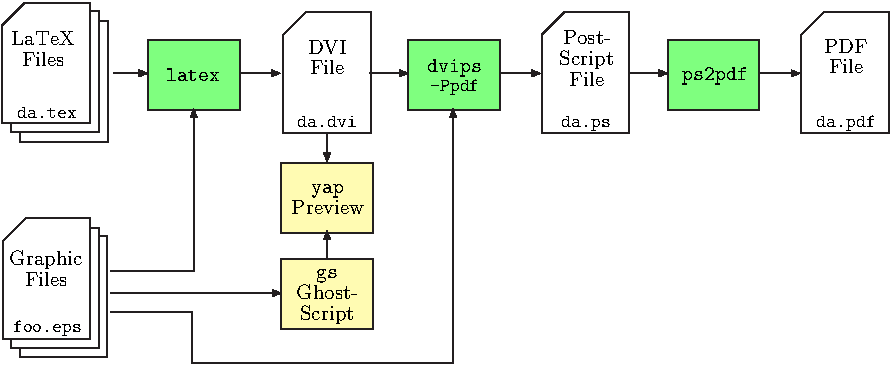
\includegraphics[width=1.0\textwidth]{workflow-cm}
\caption{Erzeugung von
PDF-Doku\-men\-ten im DVI-PS-Workflow. EPS-Grafiken werden erst bei der
Erzeugung der PS-Datei eingebunden. 
Anmerkung: Die abgebildete Vektorgrafik wurde mit \emph{Freehand} unter
Verwendung der \emph{BaKoMa} TrueType-Schriften erstellt %
(s.\ Abschn.\ \ref{sec:tex-schriften-in-grafiken}).}
\label{fig:latex-pdf-workflow}
\end{figure}

\end{comment}


\section{Drucken}

Vor dem Drucken der Arbeit empfiehlt es sich, einige Dinge zu beachten, um unnötigen Aufwand (und auch Kosten) zu vermeiden.

\subsection{Drucker und Papier}

Die Abschlussarbeit sollte in der Endfassung unbedingt auf einem
qualitativ hochwertigen Laserdrucker ausgedruckt werden, Ausdrucke
mit Tintenstrahldruckern sind \emph{nicht} ausreichend. Auch das
verwendete Papier sollte von guter Qualität (holzfrei) und
üblicher Stärke (mind.\ $80\; {\mathrm g} / {\mathrm m}^2$) sein.
Falls \emph{farbige} Seiten notwendig sind, sollte man diese einzeln%
\footnote{Tip: Mit \emph{Adobe Acrobat} lassen sich sehr einfach einzelne Seiten
des Dokuments für den Farbdruck auswählen und zusammenstellen.}
auf einem Farb-Laserdrucker ausdrucken und dem Dokument beifügen.

Übrigens sollten \emph{alle} abzugebenden Exemplare \textbf{gedruckt} (und nicht kopiert) werden! Die Kosten für den Druck
sind heute nicht höher als die für Kopien, der
Qualitätsunterschied ist jedoch -- \va\ bei Bildern und Grafiken
-- meist deutlich.


\subsection{Druckgröße}

Zunächst sollte sichergestellt werden, dass die in der fertigen PDF-Datei eingestellte
Papiergröße tatsächlich \textbf{A4} ist! Das geht \zB\ mit \emph{Adobe Acrobat}
oder \emph{SumatraPDF}
über \texttt{File} $\rightarrow$ \texttt{Properties},
wo die Papiergröße des Dokuments angezeigt wird:
\begin{center}
\textbf{Richtig:} A4 = $8{,}27 \times 11{,}69$ in \bzw\ $21{,}0 \times 29{,}7$ cm.
\end{center}
Falls das nicht stimmt, ist vermutlich irgendwo im Workflow versehentlich \textbf{Letter} 
als Papierformat eingestellt, %, häufig ist \emph{Adobe Distiller} "schuld".


Ein häufiger und leicht zu übersehender Fehler beim Ausdrucken von
PDF-Doku\-menten wird durch die versehentliche Einstellung der
Option "Fit to page" im Druckmenü verursacht, wobei die Seiten
meist zu klein ausgedruckt werden. Überprüfen Sie daher die Größe
des Ausdrucks anhand der eingestellten Zeilenlänge oder mithilfe
einer Messgrafik, wie am Ende dieses Dokuments gezeigt.
Sicherheitshalber sollte diese Messgrafik bis zur
Fertigstellung der Arbeit beibehalten und die entsprechende
Seite erst ganz am Schluss zu entfernt werden.
Wenn, wie häufig der Fall, einzelne Seiten getrennt in Farbe gedruckt 
werden, so sollten natürlich auch diese genau auf die Einhaltung der Druckgröße 
kontrolliert werden!




\section{Binden}

Die Endfassung der Abschlussarbeit%
\footnote{Für \textbf{Bachelorarbeiten} genügt, je nach Vorgaben des Studiengangs, meist eine einfache Bindung (Copyshop oder Bibliothek).}
ist in fest gebundener Form
einzureichen.%
\footnote{An der Fakultät Hagenberg ist bei Masterarbeiten zumindest eines der
Exemplare \emph{ungebunden} abzugeben -- dieses wird später von einem
Buchbinder in einheitlicher Form gebunden und verbleibt
danach in der Bibliothek. Datenträger sind bei diesem Exemplar lose 
und \emph{ohne} Aufkleber (jedoch beschriftet) beizulegen.}
Dabei ist eine Bindung zu
verwenden, die das Ausfallen von einzelnen Seiten nachhaltig
verhindert, \zB durch eine traditionelle Rückenbindung
(Buchbinder) oder durch handelsübliche Klammerungen aus Kunststoff
oder Metall. Eine einfache Leimbindung ohne Verstärkung ist
jedenfalls \emph{nicht} ausreichend.


Falls man -- was sehr zu empfehlen ist -- die Arbeit bei einem
professionellen Buchbinder durchführen lässt, sollte man auch auf
die Prägung am Buchrücken achten, die kaum zusätzliche Kosten
verursacht. Üblich ist dabei die Angabe des Familiennamens des
Autors und des Titels der Arbeit. Ist der Titel der Arbeit zu
lang, muss man notfalls eine gekürzte  Version angeben, wie \zB:
%
\begin{center}
\setlength{\fboxsep}{3mm}
\fbox{
\textsc{Schlaumeier}
\textperiodcentered\ \textsc{Part.\ Lösungen zur allg.\ Problematik}}
\end{center}
%



\section{Elektronische Datenträger (CD-R, DVD, USB-Stick)}
Speziell bei Arbeiten im Bereich der Informationstechnik (aber
nicht nur dort) fallen fast immer Informationen an, wie Programme,
Daten, Grafiken, Kopien von Internetseiten \usw, die für eine
spätere Verwendung elektronisch verfügbar sein sollten.
Vernünftigerweise wird man diese Daten während der Arbeit bereits
gezielt sammeln und der fertigen Arbeit auf einer CD-ROM, DVD oder
einem USB-Stick beilegen. Es ist außerdem sinnvoll -- schon allein
aus Gründen der elektronischen Archivierbarkeit -- die eigene Arbeit
selbst als PDF-Datei beizulegen.%
\footnote{Auch Bilder und Grafiken könnten in elektronischer Form nützlich
sein, die \latex- oder Word-Dateien sind hingegen überflüssig.}


Falls ein elektronischer Datenträger (CD-ROM, DVD, USB-Stick) beigelegt
wird, sollte auf folgende Dinge geachtet werden:
%
\begin{enumerate}
\item Jedem abzugebenden Exemplar muss eine identische Kopie des
Datenträgers beiliegen. %
\item Verwenden Sie qualitativ hochwertige Rohlinge und überprüfen
Sie nach der Fertigstellung die tatsächlich gespeicherten Inhalte
des Datenträgers! %
\item Der Datenträger sollte in eine im hinteren Umschlag
eingeklebte Hülle eingefügt sein und sollte so zu entnehmen sein,
dass die Hülle dabei \emph{nicht} zerstört wird (die
meisten Buchbinder haben geeignete Hüllen parat). %
\item Der Datenträger muss so beschriftet sein, dass er der
Abschlussarbeit eindeutig zuzuordnen ist, am Besten durch ein
gedrucktes Label%
\footnote{Nicht beim lose abgegebenen Bibliotheksexemplar --
dieses erhält ein standardisiertes Label durch die Bibliothek.} %
oder sonst durch \emph{saubere}
Beschriftung mit
der Hand und einem feinen, wasserfesten Stift. %
\item Nützlich ist auch ein (grobes) Verzeichnis der Inhalte des
Datenträgers (wie exemplarisch in Anhang \ref{app:cdrom}).
\end{enumerate}

\chapter{Schlussbemerkungen}
\label{cha:Schluss}



%%%----------------------------------------------------------
\appendix                                            % Anhang 
%%%----------------------------------------------------------

\chapter{Technische Informationen}
\label{app:TechnischeInfos}

	% Technische Ergänzungen
\chapter{Inhalt der CD-ROM/DVD}
\label{app:cdrom}

	% Inhalt der CD-ROM/DVD
\chapter{Fragebogen}
\label{app:Fragebogen}

	% Chronologische Liste der Änderungen
\chapter{\latex-Quellkode}
\label{app:Quellcode}

	% Quelltext dieses Dokuments

%%%----------------------------------------------------------
\MakeBibliography                        % Quellenverzeichnis
%%%----------------------------------------------------------

%%% Messbox zur Druckkontrolle ------------------------------
\chapter*{Messbox zur Druckkontrolle}



\begin{center}
{\Large --- Druckgröße kontrollieren! ---}

\bigskip

\calibrationbox{100}{50} % Angabe der Breite/Hoehe in mm

\bigskip

{\Large --- Diese Seite nach dem Druck entfernen! ---}

\end{center}



%%%----------------------------------------------------------
\end{document}
%%%----------------------------------------------------------"
\end{codeexample}
%
\noindent where |main-figure0| is the picture we are currently externalizing
and |main.tex| is the main document.

As soon as ``conversion mode'' has been detected, \pgfname\ changes the output
routine. The complete file |main.tex| is processed as normal, but only the part
of the desired picture will be written to the output file, in our case
|main-figure0.pdf|. The rest of the document is silently thrown away. Of
course, such a conversion process is quite expensive since we need to do it for
every picture. Since everything except the current picture is thrown away, the
library skips all other pictures. Furthermore, any |\includegraphics| commands
which are outside of the converted \tikzname-picture will be skipped as well.
Thus, the conversion process should be much faster than typesetting the
complete document, but it still requires its time. Eventually, the call
|%%% File encoding: UTF-8
%%% äöüÄÖÜß  <-- keine deutschen Umlaute hier? UTF-faehigen Editor verwenden!

%%% Magic Comments zum Setzen der korrekten Parameter in kompatiblen IDEs
% !TeX encoding = utf8
% !TeX program = pdflatex 
% !TeX spellcheck = de_DE
% !BIB program = biber

\documentclass[master,german,smartquotes]{hgbthesis}
% Zulässige Optionen in [..]: 
%   Typ der Arbeit: diploma, master (default), bachelor, internship 
%   Hauptsprache: german (default), english
%		smartquotes: 
%%%----------------------------------------------------------

\RequirePackage[utf8]{inputenc}		% bei der Verw. von lualatex oder xelatex entfernen!

\graphicspath{{images/}}    % Verzeichnis mit Bildern und Grafiken
\logofile{logo}				% Logo-Datei = images/logo.pdf (\logofile{}, wenn kein Logo gewünscht)
\bibliography{references}  	% Biblatex-Literaturdatei (references.bib)

%%%----------------------------------------------------------
% Angaben für die Titelei (Titelseite, Erklärung etc.)
%%%----------------------------------------------------------

%%% Einträge für ALLE Arbeiten: -----------------------------
\title{Partielle Lösungen zur allgemeinen Problematik}
\author{Peter A.\ Schlaumeier}
\programname{Universal Computing}
\placeofstudy{Hagenberg}
\dateofsubmission{2019}{07}{15}	% {YYYY}{MM}{DD}

%%% Zusätzlich für eine Bachelorarbeit: ---------------------
\thesisnumber{XXXXXXXXXX-A}   % Stud-ID, z.B. 1310238045-A  
% (A = 1. Bachelorarbeit)
\semester{Sommersemester 2017} 
\coursetitle{Einführung in die Tiefere Problematik 1} 
\advisor{Alois B.~Treuer, Päd.\ Phil.}

%%% Restriktive Lizenformel anstatt CC (nur für Typ master) -
%\strictlicense

%%%----------------------------------------------------------
\begin{document}
%%%----------------------------------------------------------

%%%----------------------------------------------------------
\frontmatter                    % Titelei (röm. Seitenzahlen)
%%%----------------------------------------------------------

\maketitle
\tableofcontents

\chapter{Vorwort} 	% engl. Preface


Dies ist \textbf{Version \hgbDate} der \latex-Dokumentenvorlage für 
verschiedene Abschlussarbeiten an der Fakultät für Informatik, Kommunikation
und Medien der FH Oberösterreich in Hagenberg, die mittlerweile auch 
an anderen Hochschulen im In- und Ausland gerne verwendet wird.

Das Dokument entstand ursprünglich auf Anfragen von Studierenden,
nachdem im Studienjahr 2000/01 erstmals ein offizieller
\latex-Grundkurs im Studiengang Medientechnik und -design an der
FH Hagenberg angeboten wurde. Eigentlich war die Idee, die bereits
bestehende \emph{Word}-Vorlage für Diplomarbeiten "einfach" in
\latex\ zu übersetzen und dazu eventuell einige spezielle
Ergänzungen einzubauen. Das erwies sich rasch als wenig
zielführend, da \latex, \va was den Umgang mit Literatur und
Grafiken anbelangt, doch eine wesentlich andere Arbeitsweise
verlangt. Das Ergebnis ist -- von Grund auf neu geschrieben und
wesentlich umfangreicher als das vorherige Dokument --
letztendlich eine Anleitung für das Schreiben mit \latex, ergänzt
mit einigen speziellen (mittlerweile entfernten) Hinweisen für \emph{Word}-Benutzer.
Technische Details zur aktuellen Version finden sich in Anhang \ref{app:TechnischeInfos}.

Während dieses Dokument anfangs ausschließlich für die Erstellung
von Diplomarbeiten gedacht war, sind nunmehr auch  
\emph{Masterarbeiten}, \emph{Bachelor\-arbeiten} und \emph{Praktikumsberichte} 
abgedeckt, wobei die Unterschiede bewusst gering gehalten wurden.

Bei der Zusammenstellung dieser Vorlage wurde versucht, mit der
Basisfunktionalität von \latex das Auslangen zu finden und -- soweit möglich --
auf zusätzliche Pakete zu verzichten. Das ist nur zum Teil gelungen;
tat\-säch\-lich ist eine Reihe von ergänzenden "Paketen" notwendig, wobei jedoch
nur auf gängige Erweiterungen zurückgegriffen wurde.
Selbstverständlich gibt es darüber hinaus eine Vielzahl weiterer Pakete,
die für weitere Verbesserungen und Finessen nützlich sein können. Damit kann
sich aber jeder selbst beschäftigen, sobald das notwendige Selbstvertrauen und
genügend Zeit zum Experimentieren vorhanden sind.
Eine Vielzahl von Details und Tricks sind zwar in diesem Dokument nicht explizit
angeführt, können aber im zugehörigen Quelltext jederzeit ausgeforscht
werden.

Zahlreiche KollegInnen haben durch sorgfältiges Korrekturlesen und
konstruktive Verbesserungsvorschläge wertvolle Unterstützung
geliefert. Speziell bedanken möchte ich mich bei Heinz Dobler für
die konsequente Verbesserung meines "Computer Slangs", bei
Elisabeth Mitterbauer für das bewährte orthographische Auge und
bei Wolfgang Hochleitner für die Tests unter Mac~OS.

Die Verwendung dieser Vorlage ist jedermann freigestellt und an
keinerlei Erwähnung gebunden. Allerdings -- wer sie als Grundlage
seiner eigenen Arbeit verwenden möchte, sollte nicht einfach
("ung'schaut") darauf los werken, sondern zumindest die
wichtigsten Teile des Dokuments \emph{lesen} und nach Möglichkeit
auch beherzigen. Die Erfahrung zeigt, dass dies die Qualität der
Ergebnisse deutlich zu steigern vermag.

Dieses Dokument und die zugehörigen \latex-Klassen sind seit Nov.\ 2017 auf CTAN%
\footnote{Comprehensive TeX Archive Network} 
als Paket \texttt{hagenberg-thesis} verfügbar unter
%
\begin{itemize}
\item[]\url{https://ctan.org/pkg/hagenberg-thesis}.
\end{itemize}
%
Den jeweils aktuellen Quelltexte sowie zusätzliche Materialien findet man unter
%
\begin{itemize}
\item[]\url{https://github.com/Digital-Media/HagenbergThesis}.%
\footnote{Unter \url{https://github.com/Digital-Media/HagenbergThesis/blob/master/CHANGELOG.md}
sowie genauer unter \url{https://github.com/Digital-Media/HagenbergThesis/commits/master} 
findet man auch eine (früher im Anhang dieses Dokuments enthaltene) chronologische Auflistung der 
Änderungen.}
\end{itemize}



\noindent
Trotz großer Mühe enthält ein Dokument wie dieses immer Fehler und Unzulänglichkeiten
-- Kommentare, Verbesserungsvorschläge und sinnvolle Ergänzungen
sind daher willkommen, am einfachsten als Kommentar oder Fehlermeldung ("Issue") 
auf GitHub oder jederzeit auch per E-Mail an
%
\begin{itemize}
\item[]
Dr.\ Wilhelm Burger, Department für Digitale Medien,\newline
Fachhochschule Oberösterreich, Campus Hagenberg (Österreich)\newline
\nolinkurl{wilhelm.burger@fh-hagenberg.at}
\end{itemize}

\noindent
Übrigens, hier im Vorwort (das bei Diplom- und Masterarbeiten üblich, bei Bachelorarbeiten 
aber entbehrlich ist) kann kurz auf die Entstehung des Dokuments eingegangen werden.
Hier ist auch der Platz für allfällige Danksagungen (\zB an den Betreuer, 
den Begutachter, die Familie, den Hund, \ldots), Widmungen und philosophische 
Anmerkungen. Das sollte man allerdings auch nicht übertreiben und auf 
einen Umfang von maximal zwei Seiten beschränken.




 % Optional. Ggf. weglassen
\chapter{Kurzfassung}

\begin{german}
An dieser Stelle steht eine Zusammenfassung der Arbeit, Umfang
max.\ 1 Seite. 
...
\end{german}		
This document gives a quick, relatively minimal example of the use of
\texttt{uafthesis.cls}, while trying to show its features.

This section is contained in \texttt{abstract.tex}.
			

%%%----------------------------------------------------------
\mainmatter          % Hauptteil (ab hier arab. Seitenzahlen)
%%%----------------------------------------------------------

\chapter{Einleitung}
\label{cha:Einleitung}

\section{Zielsetzung}
Dieses Dokument ist als vorwiegend technische Starthilfe für das
Erstellen einer Masterarbeit (oder Bachelorarbeit) mit \latex
gedacht und ist die Weiterentwicklung einer früheren
Vorlage\footnote{Nicht mehr verfügbar.} für das Arbeiten mit
Microsoft \emph{Word}. Während ursprünglich daran gedacht war, die
bestehende Vorlage einfach in \latex zu übernehmen, wurde rasch
klar, dass allein aufgrund der großen Unterschiede zum Arbeiten
mit \emph{Word} ein gänzlich anderer Ansatz notwendig wurde. Dazu
kamen zahlreiche Erfahrungen mit Diplomarbeiten in den
nachfolgenden Jahren, die zu einigen zusätzlichen Hinweisen Anlass gaben.

Das vorliegende Dokument dient einem zweifachen Zweck: 
\emph{erstens} als Erläuterung und Anleitung, \emph{zweitens} als
direkter Ausgangspunkt für die eigene Arbeit. Angenommen wird,
dass der Leser bereits über elementare Kenntnisse im Umgang mit
\latex verfügt. In diesem Fall sollte -- eine einwandfreie
Installation der Software vorausgesetzt -- der Arbeit nichts mehr
im Wege stehen. Auch sonst ist der Start mit \latex\ nicht
schwierig, da viele hilfreiche Informationen auf den zugehörigen
Webseiten zu finden sind (s.\ Kap.~\ref{cha:ArbeitenMitLatex}).





\section{Warum {\latex}?}

Diplomarbeiten, Dissertationen und Bücher im
technisch-natur\-wissen\-schaft\-lichen Bereich werden
traditionell mithilfe des Textverarbeitungssystems \latex
\cite{Lamport1994, Lamport1995} gesetzt. Das hat gute Gründe, denn
\latex ist bzgl.\ der Qualität des Druckbilds, des Umgangs mit
mathematischen Elementen, Literaturverzeichnissen etc.\
unübertroffen und ist noch dazu frei verfügbar. Wer mit \latex
bereits vertraut ist, sollte es auch für die Abschlussarbeit
unbedingt in Betracht ziehen, aber auch für den Anfänger sollte
sich die zusätzliche Mühe am Ende durchaus lohnen.

Für den professionellen elektronischen Buchsatz wurde früher
häufig \emph{Adobe Framemaker} verwendet, allerdings ist diese
Software teuer und komplex. Eine modernere Alternative dazu ist
\emph{Adobe InDesign}, wobei allerdings die Erstellung
mathematischer Elemente und die Verwaltung von Literaturverweisen
zur Zeit nur rudimentär unterstützt werden.%
\footnote{Angeblich werden aber für den (sehr sauberen) Schriftsatz 
in \emph{InDesign} ähnliche Algorithmen wie in \latex\ verwendet.}

Microsoft \emph{Word} gilt im Unterschied zu \latex, 
\emph{Framemaker} und \emph{InDesign} übrigens nicht als professionelle
Textverarbeitungssoftware, obwohl es immer häufiger auch von
großen Verlagen verwendet wird.%
\footnote{Siehe auch \url{http://latex.tugraz.at/mythen.php}.}
Das Schriftbild in \emph{Word}
lässt -- zumindest für das geschulte Auge -- einiges zu wünschen
übrig und das Erstellen von Büchern und ähnlich großen Dokumenten
wird nur unzureichend unterstützt. Allerdings ist \emph{Word} sehr
verbreitet, flexibel und vielen Benutzern zumindest oberflächlich
vertraut, sodass das Erlernen eines speziellen Werkzeugs wie
\latex\ ausschließlich für das Erstellen einer Abschlussarbeit
manchen verständlicherweise zu mühevoll ist. Es sollte daher
niemandem übel genommen werden, wenn er/sie sich auch bei der Abschlussarbeit
auf \emph{Word} verlässt. Im Endeffekt lässt sich mit etwas
Sorgfalt (und ein paar Tricks) auch damit ein durchaus akzeptables
Ergebnis erzielen. 
Ansonsten sollten auch für \emph{Word}-Benutzer 
einige Teile dieses Dokuments von Interesse sein, insbesondere die
Abschnitte über Abbildungen und Tabellen
(Kap.~\ref{cha:Abbildungen}) und mathematische Elemente
(Kap.~\ref{cha:Mathematik}).


\section{Aufbau der Arbeit}

Hier am Ende des Einleitungskapitels (und nicht
etwa in der Kurzfassung) ist der richtige Platz, um die
inhaltliche Gliederung der nachfolgenden Arbeit zu beschreiben.
Hier sollte man darstellen, welche Teile (Kapitel) der Arbeit
welche Funktion haben und wie sie inhaltlich zusammenhängen. Auch
die Inhalte des \emph{Anhangs} -- sofern vorgesehen -- sollten hier
kurz beschrieben werden.

Zunächst sind in Kapitel \ref{cha:Abschlussarbeit} einige wichtige
Punkte zu Abschlussarbeiten im Allgemeinen zusammengefasst.
Kapitel \ref{cha:ArbeitenMitLatex} beschreibt die Idee und die
grundlegenden technischen Eigenschaften von \latex.
Kapitel \ref{cha:Abbildungen} widmet sich der Erstellung von Abbildungen
und Tabellen sowie der Einbindung von Quellcode.
Mathematische Elemente und Gleichungen sind das Thema in Kapitel \ref{cha:Mathematik} 
\usw
Anhang \ref{app:TechnischeInfos} enthält technische Details zu
dieser Vorlage, 
Anhang \ref{app:cdrom} enthält eine Auflistung von zugehörigen Materialien
auf einem beigelegten Speichermedium, und 
Anhang \ref{app:Fragebogen} zeigt ein Beispiel für die
Einbindung eines mehrseitigen PDF-Dokuments.







\chapter{Die Abschlussarbeit}
\label{cha:Abschlussarbeit}

Jede Abschlussarbeit%
\footnote{Die meisten der folgenden Bemerkungen gelten gleichsam für Bachelor-, Master- und Diplomarbeiten.} 
ist anders und dennoch sind sich gute
Arbeiten in ihrer Struktur meist sehr ähnlich, \va\ bei
technisch-natur\-wissen\-schaft\-lichen Themen. 

\section{Elemente der Abschlussarbeit}

Als Ausgangspunkt bewährt hat sich der folgende Grundaufbau, der natürlich 
vari\-iert und beliebig verfeinert werden kann:
%
\begin{enumerate}
\item \textbf{Einführung und Motivation}: Was ist die Problem- oder Aufgabenstellung und
warum sollte sich jemand dafür interessieren?
\item \textbf{Präzisierung des Themas}: Hier wird der aktuelle Stand der Technik
oder Wissenschaft ("State-Of-The-Art") beschrieben, es werden bestehende
Defizite oder offene Fragen aufgezeigt und daraus die
Stoßrichtung der eigenen Arbeit entwickelt.
\item \textbf{Eigener Ansatz}: Das ist natürlich der Kern der Arbeit. Hier
wird gezeigt, wie die vorher beschriebene Aufgabenstellung gelöst und --
häufig in Form eines Programms%
\footnote{\emph{Prototyp} ist in diesem Zusammenhang ein gerne benutzter Begriff, der im Deutschen
allerdings oft unrichtig dekliniert wird. Richtig ist: der \emph{Prototyp}, des \emph{Prototyps}, dem/den \emph{Protototyp} -- falsch hingegen \zB: des \emph{Prototyp\underline{en}}!
} --
realisiert wird, ergänzt durch illustrative Beispiele.
\item \textbf{Zusammenfassung}: Was wurde erreicht und welche Ziele sind
noch offen geblieben, wo könnte weiter gearbeitet werden?
\end{enumerate}
%
Natürlich ist auch ein gewisser dramaturgischer Aufbau der Arbeit
wichtig, wobei zu bedenken ist, dass der Leser in der Regel nur
wenig Zeit hat und -- anders als etwa bei einem Roman -- seine
Geduld nicht auf die lange Folter gespannt werden darf. Erklären
Sie bereits in der Einführung (und nicht erst im letzten Kapitel),
wie Sie an die Sache herangehen, welche Lösungen Sie vorschlagen
und wie erfolgreich Sie damit waren.

Übrigens, auch Fehler und Sackgassen dürfen (und sollten)
beschrieben werden; ihre Kenntnis hilft oft doppelte Experimente und
weitere Fehler zu vermeiden und ist damit sicher nützlicher als
jede Schönfärberei.
Und natürlich ist es auch nicht verboten, seine eigene Meinung 
in sachlicher Form zu äußern.


\section{Arbeiten in Englisch}
\label{sec:englisch}

Diese Vorlage ist zunächst darauf abgestellt, dass die
Abschlussarbeit in deutscher Sprache erstellt wird. Vor allem bei
Arbeiten, die in Zusammenarbeit mit größeren Firmen oder
internationalen Instituten entstehen, ist es häufig erwünscht,
dass die Abschlussarbeit zu besseren Nutzbarkeit in englischer
Sprache verfasst wird, und viele Hochschulen%
\footnote{Die FH Oberösterreich macht hier keine Ausnahme. 
Der Begriff "Fachhochschule" wird dabei entweder gar nicht
übersetzt oder -- wie im deutschsprachigen Raum mittlerweile üblich -- 
mit \emph{University of Applied Sciences}.
%Die offizielle englische Übersetzung von "Medientechnik und -design"
%ist übrigens \emph{Media Technology and Design}.
} 
lassen dies in
der Regel auch zu.

Beachtet sollte allerdings werden, dass das Schreiben dadurch nicht
einfacher wird, auch wenn einem Worte und Sätze im Englischen
scheinbar leichter "aus der Feder" fließen. Gerade im Bereich
der Informatik erscheint durch die Dominanz englischer
Fachausdrücke das Schreiben im Deutschen mühsam und das Ausweichen
ins Englische daher besonders attraktiv. Das ist jedoch
trügerisch, da die eigene Fertigkeit in der Fremdsprache
(trotz der meist langjährigen Schulbildung) häufig überschätzt wird.
Prägnanz und Klarheit gehen leicht verloren und bisweilen ist das
Resultat ein peinliches Gefasel ohne Zusammenhang und soliden
Inhalt. Sofern die eigenen Englischkenntnisse nicht wirklich gut sind, ist
es ratsam, zumindest die wichtigsten Teile der Arbeit zunächst in
Deutsch zu verfassen und erst nachträglich zu übersetzen. Besondere Vorsicht ist bei der Übersetzung von scheinbar
vertrauten Fachausdrücken angebracht. Zusätzlich ist es immer zu
empfehlen, die fertige Arbeit von einem "native speaker"
korrigieren zu lassen.



Technisch ist, außer der Spracheinstellung und den
unterschiedlichen Anführungszeichen (s.\
Abschn.~\ref{sec:anfuehrungszeichen}), für eine englische Arbeit
nicht viel zu ändern, allerdings sollte Folgendes beachtet werden:
%
\begin{itemize}
\item  Die Titelseite (mit der Bezeichnung "Diplomarbeit" oder "Masterarbeit") 
ist für die einzureichenden Exemplare jedenfalls in \emph{deutsch} zu halten,
auch wenn der Titel englisch ist. 
\item Ebenso muss neben dem
englischen \emph{Abstract} auch eine deutsche \emph{Kurzfassung}
enthalten sein. %
\item Akademische Titel von Personen haben im Englischen offenbar
weniger Bedeutung als im Deutschen und werden daher meist
weggelassen.
\end{itemize}

\chapter{Zum Arbeiten mit \latex}
\label{cha:ArbeitenMitLatex}

\section{Einstieg}
\label{sec:LatexEinstieg}

\latex ist eine in den Naturwissenschaften sehr verbreitete
und mittlerweile klassische Textverarbeitungssoftware für das Erstellen
großer und komplizierter Dokumente mit professionellem Anspruch.
Das Arbeiten mit \latex erscheint -- zumindest für den ungeübten Benutzer -- %
zunächst schwieriger als mit herkömmlichen Werkzeugen für die
Textverarbeitung.

Zum Ersten ist -- im Unterschied zu den meisten gängigen
Text\-ver\-arbei\-tungs\-prog\-ram\-men -- \latex nicht \textsc{Wysiwyg}%
\footnote{"What You See Is What You Get." Es gibt auch 
\textsc{Wysiwyg}-Implementierungen für \latex, 
\zB\ \emph{Scientific WorkPlace} (\url{https://www.mackichan.com/}) oder
\emph{LyX} (\url{https://www.lyx.org/}), 
die aber teuer \bzw\ relativ langsam sind.},
sondern es handelt sich um eine \emph{Markup Lang\-uage} (wie HTML) -- noch dazu
eine für den Anfänger recht komplizierte -- und zugehörige Werkzeuge.
Ungewohnt erscheinen sicher auch die vermeintlich starken
Einschränkungen von \latex,
insbesondere in Bezug auf die Wahl der Schriften und das
Layout. Während anfangs of der Eindruck entsteht, dass diese Rigidität
die eigene Kreativität beschränkt, fällt mit der Zeit auf, dass es gerade
dadurch gelingt, sich stärker auf die Inhalte der Arbeit zu
konzentrieren als auf deren äußere Form. Dass am Ende die Form dennoch stimmt,
ist allerdings nur dann gewährleistet, wenn man sich bei den eigenen Modifikationen
der Formate und Parameter äußerste Zurückhaltung auferlegt, es sei denn,
man ist in der Zwischenzeit bereits selbst zum \latex-\emph{Guru} avanciert.

Insgesamt lohnt sich der Aufwand, wie viele meinen, zumal die Abschlussarbeit
in jedem Fall (mit oder ohne \latex) ein substantielles Stück Arbeit ist.
Allerdings sollte mithilfe von \latex ein professionell aussehendes
Ergebnis einfacher zu erreichen sein und es dürfte wohl auch einiger
Ärger mit Fehlern und Einschränkungen gängiger Software erspart bleiben.
Zudem könnte es durchaus sein, dass sich nebenbei auch das eigene Auge für
die Feinheiten des Buchsatzes (weiter-){\obnh}entwickelt.%
\footnote{Dieses abschließende Textelement wurde übrigens zur Ermöglichung eines 
Zeilenumbruchs nach der Klammer so gesetzt: \texttt{\ldots (weiter-)\{{\bs}optbreaknh\}entwickelt.}
Das Makro \texttt{{\bs}optbreaknh} ("optional break with no hyphen") ist in 
\texttt{hgb.sty} definiert.}


\subsection{Software}
\label{sec:Software}

Zum Arbeiten mit \latex wird -- neben einem Computer -- natürlich Software benötigt. Mussten früher oft die einzelnen Komponenten von \latex mühevoll zusammengesucht und für die eigene Umgebung konfiguriert werden, gibt es mittlerweile für die wichtigsten Plattformen (Windows, Mac~Os, Linux) fertige \latex-Installationen, die ohne weiteres Zutun laufen. Die aktuelle Version von \latex\ ist \LaTeXe\ (sprich "LaTeX zwei e"). 
Zum Arbeiten mit \latex\ werden zwei Dinge benötigt:
%
\begin{itemize}
\item \latex-Installation (Distribution),
\item Texteditor oder Autorenumgebung (Frontend).
%\item PostScript/PDF-Software 
\end{itemize}
%
Sämtliche Komponenten sind kostenlos und für alle gängigen Plattformen verfügbar.


\subsubsection{Windows}
\label{sec:Windows}

Unter \emph{Windows} (XP und höher) hat sich folgendes Setup bewährt,
mit dem \ua auch dieses Dokument erstellt wurde:
%
\begin{itemize}
\item \textbf{\latex-Distribution}: \emph{MikTeX 2.9}\footnote{\url{https://miktex.org/}} oder höher.
MikTeX enthält bereits alle notwendigen Hilfsprogramme, wie beispielsweise \texttt{pdflatex}.

\item \textbf{PDF-Viewer}: \emph{SumatraPDF}.%
\footnote{\url{https://www.sumatrapdfreader.org/}}

\item \textbf{Frontend}: \emph{TeXnicCenter}.%
\footnote{\url{http://www.texniccenter.org/}}
Grundsätzlich kann jeder Texteditor%
\footnote{Unter Windows \zB\ \emph{Notepad++} (\url{https://notepad-plus-plus.org/}).}
verwendet werden, praktischer ist jedoch eine integrierte \latex-Um\-geb\-ung wie TeXnicCenter, die einen auch bei 
der Dateiverwaltung, der Verarbeitung der Dokumente und der Fehlerbehandlung unterstützt.
Eine interessante Alternative bietet die Verwendung von \emph{Eclipse}\footnote{\url{https://www.eclipse.org/}}
als plattformunabhängiges Frontend 
(mit dem \emph{TeXlipse}\footnote{\url{https://projects.eclipse.org/projects/science.texlipse}} Plugin).
\end{itemize}
%
Beim erstem Mal sollten \emph{MikTeX}, \emph{SumatraPDF} und \emph{TeXnicCenter} in genau dieser Reihenfolge installiert werden.

Als Gesamtpaket bietet sich \emph{TeXstudio}\footnote{\url{https://www.texstudio.org/}} an. 
In diesem Fall kann die Installation eines separaten PDF-Viewers entfallen, denn dieser ist in der 
Software bereits enthalten.

\subsubsection{Mac~OS}
\label{sec:MacOs}

Unter Mac~OS~X ist die Referenzdistribution \emph{MacTeX}.%
\footnote{\url{https://www.tug.org/mactex/}} 
Sie enthält neben der TeX-Distribution \emph{TeX Live} auch gängige Editoren wie \emph{TeXWorks} oder \emph{TeXshop}. Mit dem \emph{TeX Live Utility} können Pakete verwaltet und die Distribution auf den neuesten Stand gebracht werden. Als Alternative zu den beiden genannten Editoren steht \emph{TeXnicle}%
\footnote{\url{http://www.bobsoft-mac.de/texnicle/texnicle.html}} zur Verfügung. Er bietet -- ähnlich wie \emph{TeXnicCenter} unter Windows -- einen projektbasierten Workflow an.
Ebenso ist auch \emph{TeXstudio} für Mac~OS~X 10.8 und neuer verfügbar.
Ein PDF-Viewer muss unter Mac~OS~X übrigens nicht extra installiert werden. Alle genannten Editoren beinhalten eine eigene PDF-Vorschau.


\subsubsection{Linux}

Auch unter Linux ist \emph{TeX Live} (\so) eine häufig verwendete TeX-Distri\-bution. 
Als Frontend sind beispielsweise
\emph{Lyx}\footnote{\url{https://www.lyx.org/}},
\emph{Kile}\footnote{\url{https://kile.sourceforge.io/}} und
\emph{Texmaker}\footnote{\url{http://www.xm1math.net/texmaker/}} 
verbreitet.
\emph{TeXstudio} ist ebenfalls für alle gängigen Distributionen über die jeweiligen Paket-Manager erhältlich. Alternativ können die entsprechenden Packages von der Webseite bezogen werden.
In manchen gängigen Linux-Versionen ist bereits eine komplette \latex-Distribution enthalten, sodass im besten Fall überhaupt keine zusätzliche Installation notwendig ist.  


\subsection{Literatur}
\label{sec:literatur}

Es ist müßig, ohne geeignete Literatur mit \latex zu beginnen, selbst
fortgeschrittene Benutzer werden immer wieder auf Hilfe angewiesen
sein. Erfreulicherweise ist sehr viel Nützliches auch online verfügbar.
Gute Startpunkte sind \zB
%
\begin{itemize}
\item \emph{\textrm{\LaTeXe}-Kurzbeschreibung} von Daniel et al.\ \cite{Daniel2018}
\item \emph{The Not So Short Introduction to \textrm{\LaTeXe}}
            von Oetiker et al.\ \cite{Oetiker2018}
\end{itemize}
%
\noindent
Als mittlerweile bereits klassisches Handbuch zu \latex ist
%
\begin{itemize}
  \item \emph{A Guide to \textrm{\LaTeX}} von H.~Kopka und P.~Daly \cite{Kopka2003}
\end{itemize}
%
zu empfehlen, zu dem es für Interessierte auch zwei vertiefende
Zusatzbände in Deutsch gibt. Zahlreiche weitere Dokumente zu
\latex und verwandten Themen finden sich \ua im Rahmen des {\em
Comprehensive TeX Archive Network} (CTAN) auf
\begin{quote}
	\url{https://www.ctan.org/}%
	\footnote{\url{https://www.ctan.org/topic/}}
\end{quote}
%
Besonders nützlich sind auch die
\emph{Comprehensive List of \textrm{\latex} Symbols} \cite{Pakin2017}
und die Beschreibungen wichtiger \latex-Pakete, wie
%
\begin{quote}
  \texttt{babel} \cite{Bezos2018},\newline
  \texttt{graphics}, \texttt{graphicx} \cite{Carlisle2017},\newline
  \texttt{fancyhdr} \cite{Oostrum2019},\newline
  \texttt{caption} \cite{Sommerfeldt2011}.
\end{quote}


\section{Schrift}

In einem \latex-Dokument muss zunächst die verwendete Schriftart festgelegt werden. Im Text können dann mittels diverser Auszeichnungen Textstellen durch eine Änderung des Schriftstils hervorgehoben werden.

\subsection{Schriftarten}

\latex verwendet normalerweise die Schriften der \emph{Computer
Modern}
(CM) Serie, die so wie die \emph{TeX}-Software selbst von Donald Knuth%
\footnote{\url{http://www-cs-faculty.stanford.edu/~uno/}} entwickelt
wurden. Die drei Basis-Schrifttypen der CM-Serie in \latex sind
%
\begin{quote}
\begin{tabular}{lcl}
\textrm{Roman}      & & \verb!\textrm{Roman}!,\\
\textsf{Sans Serif} & & \verb!\textsf{Sans Serif}!,\\
\texttt{Typewriter} & & \verb!\texttt{Typewriter}!.\\
\end{tabular}
\end{quote}
%
\noindent In den Augen vieler Benutzer ist allein die Qualität und
Zeitlosigkeit dieser Schriften ein Grund, \latex für seriöse
Zwecke zu verwenden. Ein weiterer Vorteil der \emph{TeX}-Schriften
ist, dass die unterschiedlichen Schriftfamilien und Schnitte
bezüglich der Größe sehr gut aufeinander abgestimmt sind.

Darüber hinaus können aber in \latex auch beliebige 
\emph{PostScript}-Schrif\-ten (Type 1) verwendet werden, was allerdings in
der Praxis einiges an "Tuning"-Arbeit verlangt. Häufig verwendet
werden \zB\ \emph{Times} und \emph{Palatino}, derzeit ist aber ein Trend 
zurück zu den klassischen CM-Schriften zu beobachten.



\subsection{Texte hervorheben}

Texte können auf unterschiedliche Weise aus dem Fließtext hervorgehoben werden.
\begin{itemize}
%
\item Die Auszeichnung in \textit{Kursivschrift} oder "italic" (\verb!\textit{..}!) ist \va\ zum Hervorheben von
Betonungen und Zitaten geeignet, aber auch für
Produktbezeichnungen, Fremdwörter und Variablen im Text, \zB
%
\begin{quote}
\verb!\textit{Variable}! $\rightarrow$ \textit{Variable}
\end{quote}
%
\item \textsl{Slanted} %
(\verb!\textsl{..}!) bedeutet eine geneigte Schrift und
unterscheidet sich damit deutlich von \textit{Italic}; 
zum Vergleich:
%
\begin{quote}
\verb!\textrm{Daimler-Chrysler}! $\rightarrow$ \textrm{Daimler-Chrysler} \newline%
\verb!\textsl{Daimler-Chrysler}! $\rightarrow$ \textsl{Daimler-Chrysler} \newline%
\verb!\textit{Daimler-Chrysler}! $\rightarrow$ \textit{Daimler-Chrysler}
\end{quote}
%
\item \textbf{Boldface} (\verb!\textbf{..}!) wird \ia\ verwendet für 
\textbf{Überschriften}, Bezeichnungen von \textbf{Abbildungen} und 
\textbf{Tabellen}, im Fließtext aber selten:
%
\begin{quote}
\verb!\textbf{Überschriften}! $\rightarrow$ \textbf{Überschriften}
\end{quote}
%
\item \emph{Emphasize} (\verb!\emph!) %
ist normalerweise gleichbedeutend mit \verb!\textit!, wobei
\verb!\emph! allerdings auch bei geschachtelten
Hervorhebungen und im Bereich anderer Schriftschnitte das
"Richtige" tut: 
%
\begin{quote}
\setlength{\tabcolsep}{0pt}%
\begin{tabular}{lcl}
\verb!\textrm{Du \emph{auch} hier?}! & $\;\rightarrow\;$ &
    \textrm{Du \emph{auch} hier?}
\\
\verb!\textit{Du \emph{auch} hier?}! & $\;\rightarrow\;$ &
    \textit{Du \emph{auch} hier?} 
\\
\verb!\textsl{Du \emph{auch} hier?}! & $\;\rightarrow\;$ & 
    \textsl{Du \emph{auch} hier?}
\\
\verb!\textbf{Du \emph{auch} hier?}! & $\;\rightarrow\;$ & 
    \textbf{Du \emph{auch} hier?}
\\
\verb!\texttt{Du \emph{auch} hier?}! & $\;\rightarrow\;$ & 
    \texttt{Du \emph{auch} hier?}
\end{tabular}
\end{quote}
%
\item \underline{Unterstreichungen} sind ein Relikt aus der 
Schreibmaschinenära und im modernen Schriftsatz
eigentlich \underline{überflüssig}. Sie sollten daher nur in
Ausnahmefällen verwendet werden, \zB
%
\begin{quote}
\verb!\underline{überflüssig}!%
\footnote{Unterstrichene Texte werden zudem nicht automatisch abgeteilt.}
\end{quote}
%
\end{itemize}



\section{Textstruktur}

Zur Strukturierung des eigenen Text stellt \latex eine Reihe von Auszeichnungen zur Verfügung.

\subsection{Absatztrennung}

Absätze werden in {\latex}-Quelltext ausschließlich durch das
Einfügen einer oder mehrerer \textbf{Leerzeilen} voneinander
getrennt, es sind also \emph{keinerlei sonstige Steueranweisungen}
notwendig!
%
\begin{center}
\setlength{\fboxrule}{0.2mm}
\setlength{\fboxsep}{2mm}
\fbox{%
\begin{minipage}{0.9\textwidth}
Besonders die Verwendung von \texttt{\textbackslash\textbackslash} und 
 \texttt{\textbackslash{newline}}
Anweisungen zur Absatztrennung ist ein häufig zu beobachtender \textbf{Fehler}. 
Vor normalen Absätzen auch \emph{nichts} verloren hat die
Anweisung \texttt{\textbackslash{paragraph}\{\}}
-- sie ist in \latex\ (im Unterschied zu HTML)
eine Markierung für Überschriften mit Titel (\su)!
\end{minipage}}
\end{center}

Üblicherweise wird von {\latex} zwischen aufeinanderfolgenden 
Ab\-sätzen \emph{kein} zusätzlicher vertikaler Abstand eingefügt.%
\footnote{Das ist die Standardeinstellung in {\latex} und
natürlich abhängig von der verwendeten Dokumentenklasse, Style
etc.} 
Allerdings wird die
\emph{erste} Zeile jedes Absatzes (mit Ausnahme des ersten Absatzes
eines Abschnitts) eingerückt, um so die Absatzgrenzen deutlich zu
machen. Dieses Schema hat sich nicht nur im traditionellen
Buchsatz bewährt%
\footnote{Wer es nicht glaubt, sollte sein Bücherregal (oder notfalls das seiner Eltern) nach Gegenbeispielen durchsuchen.}
und sollte auch beibehalten werden, es sei denn
es gibt wirklich \emph{sehr} gute Gründe dagegen.
Für alle übrigen Gliederungen im vertikalen Textfluss sind Überschriften (s.\ unten) vorgesehen.

% Note: as of 2017-06-12 the \SuperPar macro has been deactivated
%\SuperPar 
%Manchmal besteht allerdings der Wunsch, etwa zur Verdeutlichung eines inhaltlichen Sprungs \emph{zwischen} zwei Absätzen einen zusätzlichen Abstand einzufügen, ohne dabei eine neue Überschrift zu setzen. Das kann gegebenenfalls (wie vor dem aktuellen Absatz passiert) durch 
%%
%\begin{quote}
%\texttt{{\bs}SuperPar} \emph{Manchmal besteht allerdings der Wunsch, \ldots}
%\end{quote}
%%
%erreicht werden, sollte jedoch sehr sparsam und wirklich \textbf{nur in begründbaren Einzelfällen} verwendet werden.%
%\footnote{Das Makro \texttt{{\bs}SuperPar} ist in \texttt{hgb.sty} definiert.}




\subsection{Überschriften}
\label{sec:ueberschriften}

\latex\ bietet -- abhängig von der verwendeten Dokumentenklasse --
einen Satz vordefinierter Überschriftformate in folgender Ordnung:
%
\begin{quote}
\verb!\part{!\texttt{\em Titel}\verb!}!%
\footnote{\texttt{part} ist für die Gliederung eines
größeren Werks in mehrere Teile vorgesehen und wird üblicherweise
bei einer Abschlussarbeit (und auch in diesem Dokument) nicht
verwendet.}
\newline%
\verb!\chapter{!\texttt{\em Titel}\verb!}! \newline%
\verb!\section{!\texttt{\em Titel}\verb!}! \newline%
\verb!\subsection{!\texttt{\em Titel}\verb!}! \newline%
\verb!\subsubsection{!\texttt{\em Titel}\verb!}! \newline%
\verb!\paragraph{!\texttt{\em Titel}\verb!}! \newline%
\verb!\subparagraph{!\texttt{\em Titel}\verb!}!
\end{quote}
%

\paragraph{Häufiger Fehler:} Bei \verb!\paragraph{}! und
\verb!\subparagraph{}! läuft -- wie in diesem Absatz zu sehen --
der dem Titel folgende Text ohne Umbruch in der selben Zeile
weiter, weshalb im Titel auf eine passende Interpunktion (hier
\zB\ \underline{\texttt{:}}) geachtet werden sollte. Der horizontale Abstand
nach dem Titel allein würde diesen als Überschrift nicht erkennbar
machen.


\subsection{Listen}

Listen sind ein beliebtes Mittel zur Textstrukturierung. In
\latex\ sind -- ähnlich wie in HTML -- drei Arten von formatierten
Listen verfügbar: ungeordnete Auflistung ("Knödelliste"),
geordnete Auflistung (Aufzählung) und Beschreibungsliste
(Description):
%
\begin{verbatim}
    \begin{itemize}     ... \end{itemize}
    \begin{enumerate}   ... \end{enumerate}
    \begin{description} ... \end{description}
\end{verbatim}
%
Listeneinträge werden mit \verb!\item! markiert, bei \texttt{description}-Listen mit \verb!\item[!\texttt{\em titel}\verb!]!. Listen
können ineinander verschachtelt werden, wobei sich bei \texttt{itemize}- und \texttt{enumerate}-Listen die Aufzählungszeichen mit
der Schachtelungstiefe ändern (Details dazu in der
\latex-Dokumentation).


\subsection{Absatzformatierung und Zeilenabstand}

Abschlussarbeiten werden -- wie Bücher -- in der Regel einspaltig und
im Blocksatz formatiert, was für den Fließtext wegen der großen
Zeilenlänge vorteilhaft ist. Innerhalb von Tabellen kommt es
wegen der geringen Spaltenbreite jedoch häufig zu Problemen mit
Abteilungen und Blocksatz, weshalb dort ohne schlechtes
Gewissen zum Flattersatz ("ragged right") gegriffen werden sollte (wie
\zB\ in Tab.~\ref{tab:synthesis-techniques} auf Seite
\pageref{tab:synthesis-techniques}).


\subsection{Fußnoten}
Fußnoten können in \latex\ an beinahe jeder beliebigen Stelle,
jedenfalls aber in normalen Absätzen, durch die Anweisung
%
\begin{quote}
\verb!\footnote{!\texttt{\em Fußnotentext}\verb!}!
\end{quote}
%
gesetzt werden. Zwischen der \verb!\footnote!-Marke und dem davor
liegenden Text sollte grundsätzlich \emph{kein Leerzeichen} entstehen (eventuelle
Zeilen\-um\-brüche mit \verb!%! auskommentieren).
Die Nummerierung und Platzierung der Fußnoten
erfolgt automatisch, sehr große Fußnoten werden notfalls sogar auf
zwei aufeinanderfolgende Seiten umgebrochen.


\subsubsection{Fußnoten in Überschriften}

Auch das ist ab und zu nötig, ist aber \va\ deshalb kein so
einfacher Fall, weil die Fußnote in einer Überschrift nur an Ort
und Stelle aufscheinen darf, nicht aber im \emph{Inhaltsverzeichnis}! Ein
konkretes Beispiel dafür ist die Überschrift zu
Kapitel~\ref{cha:Schluss}, die folgendermaßen definiert ist:
%
\begin{quote}
\begin{verbatim}
\chapter[Schlussbemerkungen]%
        {Schlussbemerkungen%
        \protect\footnote{Diese Anmerkung ....}}%
\end{verbatim}
\end{quote}
%
Dabei ist der erste (optionale) Titel \verb![Schlussbemerkungen]!
der Eintrag im Inhaltsverzeichnis und im Seitenkopf. 
Der zweite (gleich lautende) Titel
\texttt{\{Schlussbemerkungen\}} erscheint auf der aktuellen Seite und
enthält auch den \verb!\footnote{}! Eintrag, der allerdings an
dieser Stelle durch die Direktive \verb!\protect! "geschützt"
werden muss. Die \verb!%!-Zeichen sind hier übrigens notwendig,
um eventuelle Leerzeichen, die durch Zeilenumbrüche im Quelltext
entstehen, zu eliminieren (dieser Trick wird 
in \latex\ häufig benötigt, s.\ Abschn.~\ref{sec:kommentare}). 
Ziemlich kompliziert also, und damit 
ein weiterer Grund, Fußnoten an solchen Stellen überhaupt zu vermeiden.

Generell sollte mit Fußnoten sparsam umgegangen werden, da sie den
Textfluss unterbrechen und den Leser ablenken. Insbesondere
sollten Fußnoten nicht (wie \va\ in manchen
sozialwissenschaftlichen Werken gepflegt) derart lang werden, dass
sie einen Großteil der Seite einnehmen und damit praktisch ein
zweites Dokument bilden.%
\footnote{Das führt bei Dokumenten mit vielen Fußnoten bei manchen Lesern angeblich so weit, dass sie aus Neugier (oder Versehen) regelmäßig bei den Fußnoten zu lesen beginnen und dann mühevoll die zugehörigen, kleingedruckten Verweise im Haupttext suchen.}


\subsection{Querverweise}
\label{sec:querverweise}

Zur Verwaltung von Querverweisen innerhalb eines Dokuments stellt
\latex\ einen sehr einfachen Mechanismus zur Verfügung. Zunächst
muss jede Stelle (Kapitel, Abschnitt, Abbildung, Tabelle etc.)
durch
%
\begin{quote}
\verb!\label{!\texttt{\em key}\verb!}!
\end{quote}
%
markiert werden, wobei \texttt{\em key} ein gültiges \latex-Symbol sein
muss. Damit Labels (die nur Zahlen sind) nicht verwechselt werden,
ist es üblich, sie je nach Bedeutung mit einer unterschiedlichen
Prefix zu versehen, \zB\
%
\begin{quote}
\tabcolsep0pt
\begin{tabular}{ll}
\verb!cha:!\texttt{\em kapitel}   & \ \ldots\ für Kapitel  \\
\verb!sec:!\texttt{\em abschnitt} & \ \ldots\ für Abschnitte (Sections) und Unterabschnitte \\
\verb!fig:!\texttt{\em abbildung} & \ \ldots\ für Abbildungen \\
\verb!tab:!\texttt{\em tabelle}   & \ \ldots\ für Tabellen \\
\verb!equ:!\texttt{\em gleichung} & \ \ldots\ für Formeln und Gleichungen\\
\end{tabular}
\end{quote}
%
\noindent Beispiele:\ \verb!\label{cha:Einleitung}! oder
\verb!\label{fig:Screen-1}!. Mit den Anweisungen
%
\begin{quote}
\verb!\ref{!\texttt{\em key}\verb!}! 
\hspace{1em} oder \hspace{1em} 
\verb!\pageref{!\texttt{\em key}\verb!}!
\end{quote}
%
kann an beliebiger Stelle im Dokument die zu \texttt{\em key} gehörige
Nummer bzw.\ Seitennummer eingesetzt werden, \zB\
%
\begin{quote}
\verb!.. wie in Kap.~\ref{cha:Einleitung} erwähnt ..!\\
\verb!.. der Screenshot auf Seite \pageref{fig:Screen-1} ..!
\end{quote}
%
Übrigens werden die Bezeichnungen \emph{Kapitel} und {\em
Abschnitt} auffallend oft falsch verwendet -- Kapitel haben
ausschließlich "ungebrochene" Nummern:
%
\begin{quote}
\begin{tabular}{ll}
   \textrm{Richtig:\ } & Kapitel 7 oder Abschnitt 2.3.4\\
   \textbf{Falsch:\ }  & Kapitel 7.2 oder Abschnitt 5
\end{tabular}
\end{quote}


\section{Wortabstand und Interpunktion}

Während \latex in vielen Bereichen des Schriftsatzes automatisch das bestmögliche Ergebnis zu erzielen versucht, ist im Bereich der Interpunktion Sorgfalt von Seiten des Autors gefragt.

\subsection{\emph{French Spacing}}

Im englischsprachigen Schriftsatz ist es üblich, nach jedem
Satzende einen gegenüber dem normalen Wortzwischenraum
vergrößerten Abstand einzusetzen. Obwohl dies im Deutschen und
Französischen traditionell nicht so ist, wird es wegen der
verbesserten Lesbarkeit auch hier manchmal verwendet (nicht in diesem
Dokument). Falls die englische ("nicht-französische") Satztrennung mit
zusätzlichem Abstand bevorzugt wird, ist lediglich die Zeile
%
\begin{quote}
\verb!\nonfrenchspacing!
\end{quote}
%
am Beginn des Dokuments einzusetzen. 
In diesem Fall sollte 
aber die Interpunktion innerhalb von
Sätzen (nach .\ und :) sorgfältig beachtet weren. Beispielsweise
schreibt sich "Dr.\ Mabuse" in der Form
%
\begin{quote}
\verb!Dr.\ Mabuse! oder \verb!Dr.~Mabuse!
\end{quote}
%
Im zweiten Beispiel wird mit dem \verb!~! Zeichen zudem ein Zeilenumbruch am Leerzeichen verhindert.


\subsection{Gedanken- und Bindestriche}
\label{sec:gedankenstrich}

Die Verwendung der falschen Strichlängen (mit und ohne
Zwischenraum) ist ganz allgemein eine häufige Fehlerquelle.
Bewusst unterschieden werden sollte zwischen
%
\begin{itemize}
\item kurzen Bindestrichen (wie in "Wagner-Jauregg"), %
\item Minus-Zeichen, \zB\ $-7$ (erzeugt mit \verb!$-7$!), und %
\item echten Gedankenstrichen -- wie hier (erzeugt mit \verb!--!).
\end{itemize}
%
\noindent Für das Setzen von Gedankenstrichen\footnote{Für alle
drei gibt es übrigens auch in \emph{Word} entsprechende
Sonderzeichen.} gibt es eindeutige Konventionen:
%
\begin{enumerate}
\item Im \emph{Deutschen} wird üblicherweise einer von zwei
Leerzeichen umgebener Gedankenstrich%
\footnote{Halbgeviertstrich (\emph{En Dash}).} -- wie hier (in
\latex\ mit {\verb*! -- !}) gesetzt. Dieser wird auch für die Angabe von
Zahlenintervallen (Seiten 12--19) benutzt. 
%
\item In \emph{englischen} Texten wird ein noch längerer
Gedankenstrich\footnote{Geviertstrich (\emph{Em Dash}).} \emph{ohne}
zusätzliche Leerzeichen---\emph{as we should be knowing by now}
(in \latex\ mit {\verb*!---!}) verwendet.
%
\end{enumerate}




\subsection{Kommentare}
\label{sec:kommentare}


Textteile können in \latex\ zeilenweise mit \verb!%! auskommentiert werden. Der einem 
\verb!%!-Zeichen nachfolgenden Text wird bis zum nächsten Zeilenende überlesen:
%
\begin{quote}
\verb!Das wird gedruckt. %Dieser Text wird ignoriert.!
\end{quote}
%
Häufig verwendet werden Kommentarzeichen aber auch zum Ausblenden von 
\emph{white space}, also Leerzeichen und Zeilenumbrüchen.
Folgendes Beispiel zeigt etwa, wie mit \verb!%! am Zeilenende das Entstehen
eines Leerzeichens vor einer nachfolgenden Fußnotenmarke vermieden werden kann:
%
\begin{quote}
\begin{verbatim}
In Österreich isst man sonntags Schnitzel.%
\footnote{Was die allgemein gute Kondition erklärt.}
\end{verbatim}
\end{quote}
%

\begin{sloppypar}
\noindent
Auf ähnliche Weise kann das Entstehen von ungewolltem Absatzzwischenraum durch 
den gezielten Einsatz von Kommentarzeilen vermieden werden, \zB\ vor und nach einem zentrierten
Textabschnitt:
\end{sloppypar}
%
\begin{quote}
\begin{verbatim}
... normaler Text.
%
\begin{center}
   Dieser Test ist zentriert.
\end{center}
%
Und jetzt geht es normal weiter ...
\end{verbatim}
\end{quote}
%
Darüber hinaus bietet die \verb!comment!-Umgebung die Möglichkeit, größere Text\-blöcke
in einem Stück auszublenden:
%
\begin{quote}
\begin{verbatim}
\begin{comment}
Dieser Text ...
   ... wird ignoriert.
\end{comment}
\end{verbatim}
\end{quote}




\subsection{Anführungszeichen (Hochkommas)}
\label{sec:anfuehrungszeichen}

Anführungszeichen sind eine häufige (und oft unbemerkte) Fehlerquelle und auch hier sind die Unterschiede zwischen Deutsch und Englisch (neben anderen Sprachen) zu beachten.


\subsubsection{Variante 1: Hochkommas mit der \latex-Standardeinstellung}

Mit der Standardeinstellung von \latex\ (\dah, \emph{ohne} Verwendung der 
hier hier eingestellten Dokumentenoption \texttt{\texttt{smartquotes}}, \su)
muss die Eingabe von vorderen und hinteren Hochkommas exakt nach den entsprechenden
Konventionen erfolgen.
Hier die korrekte \latex-Notation für englische und deutsche Texte:
%
\begin{quote}
\verb!``English''! $\rightarrow$ ``English'',\\
\verb!"`Deutsch"'! $\rightarrow$ {\glqq}Deutsch{\grqq}.
\end{quote}
%
Man beachte die subtilen typografischen Unterschiede zwischen den beiden Sprachen.%
\footnote{Manche Editoren (\zB\ \textsf{TeXnicCenter}) kann man so einstellen, dass
bei der Eingabe eines einfachen Hochkommas (\texttt{\textquotedbl}) die entsprechenden Zeichenfolge 
\emph{automatisch} (kontext- und sprachabhängig) eingesetzt wird.
Insbesondere in \textsf{Overleaf} ist das derzeit leider nicht möglich.}

\emph{Einfache} Anführungszeichen werden im Englischen analog erzeugt, 
im Deutschen werden dafür hingegen die Makros \verb!\glq! \bzw\ \verb!\grq! 
(German left/right quote) benötigt:
%
\begin{quote}
\verb!`English'! $\rightarrow$ `English',\\
\verb!{\glq}Deutsch{\grq}! $\rightarrow$ {\glq}Deutsch{\grq}.
\end{quote}


\subsubsection{Variante 2: Hochkommas mit der Option \texttt{\bfseries smartquotes}}

Diese Vorlage verwendet mit der Dokumentenoption \texttt{smartquotes}
ein \emph{spezielles Setup}, das auf dem \texttt{csquotes}-Paket%
\footnote{\url{https://ctan.org/pkg/csquotes}}
basiert.
Die korrekte Einsatz von Hochkommas vereinfacht sich damit deutlich, weil
abhängig von der aktuellen Spracheinstellung und der Position des Hochkommas
das jeweils richtige Zeichen eingesetzt wird.
Es genügt hier die Verwendung eines doppelten (geraden) Hochkommas \texttt{\textquotedbl}, wie \zB
%
\begin{quote}
\begin{english}\verb!"English"! $\rightarrow$ "English"\end{english}\ (bei Spracheinstellung \texttt{english}),\\
\verb!"Deutsch"! $\rightarrow$ "Deutsch" (bei Spracheinstellung \texttt{german}).
\end{quote}
%
Dabei ist zu beachten, dass die traditionelle Eingabe von Hochkommas (Variante~1, \so) in diesem Fall \emph{nicht}
zur Verfügung steht. Die gemischte Verwendung von Variante~1 und Variante~2 ist somit
nicht möglich! Es sind mit dieser Einstellung auch alle weiteren "shorthands" des 
\texttt{babel}-Pakets%
\footnote{\url{https://ctan.org/pkg/babel}}
(wie \zB\ \verb!"a!, \verb!"o!, \verb!"u!) \emph{permanent deaktiviert} und diese können
auch lokal nicht reaktiviert werden.%
\footnote{Die hier eingestellte Verwendung des \texttt{\textquotedbl} Zeichens als 
beidseitiges "outer quote" Zeichen gilt -- \va\ in Kombination mit der deutschen Sprache --
als "gefährlich", weil das \texttt{babel}-Paket das gerade Hochkomma für spezielle
\emph{shorthand}-Makros nutzt. Das nehmen wir mutig in Kauf, allerdings sind die 
\texttt{babel}-shorthands im aktuellen Setup generell deaktiviert um Schwierigkeiten 
zu vermeiden.}


\subsubsection{Zusätzliche Features des \texttt{csquotes}-Pakets}
Das (mit der Option \texttt{smartquotes} automatisch geladene)
\texttt{csquotes}-Paket bietet zahlreiche weitere Möglichkeiten zur 
Eingabe von zitierten Texten (Zitaten), insbesondere das Makro
%
\begin{itemize}
\item[] \verb!\enquote{text}!,
\end{itemize}
%
das den angegebenen \texttt{text} in der jeweils korrekten Form (\ua\ abhängig von der Spracheinstellung und
Verschachtelungstiefe) als Zitat auszeichnet, zum Beispiel,
%
\begin{itemize}
\item[] \verb|\enquote{Niemand hat die Absicht, eine Mauer zu bauen!}| 
\item[] $\rightarrow$ \enquote{Niemand hat die Absicht, eine Mauer zu bauen!}
\end{itemize}
%
Der Vorteil dieses Konstrukts wird besonders bei \emph{geschachtelten} Zitaten deutlich, 
wie beispielsweise in
%
\begin{itemize}
\item[] \verb|\enquote{Napoleon sagte nur \enquote{Weiter so!} und ging.}| 
\item[] $\rightarrow$ \enquote{Napoleon sagte nur \enquote{Weiter so!} und ging.}
\end{itemize}
%
Eine weiteres praktisches Feature ist das Makro \verb!\foreignquote!, mit dem man sehr einfach
fremdsprachige Zitate im Text einfügen kann, ohne die Spracheinstellung
explizit verändern zu müssen, \zB%
\footnote{Derzeit sind nur die Spracheinstellungen \texttt{german} und \texttt{english} verfügbar.}
%
\begin{itemize}
\item[] \verb|\foreignquote{english}{And God asked him: |\newline
				\verb|   \enquote{Where is Abel thy brother?} And Cain replied: \ldots}| 
\item[] $\rightarrow$ \foreignquote{english}{And God asked him: \enquote{Where is Abel thy brother?} And Cain replied: \ldots}
\end{itemize}


\section{Abteilen (Silbentrennung, \emph{Hyphenation})}
\label{subsec:layout-abteilen}

Um ein sauberes Schriftbild zu erreichen sind -- speziell im
Deutschen wegen der großen Wortlängen -- Abteilungen unerlässlich.
Die Silbentrennung erfolgt entweder \emph{automatisch} oder \emph{manuell} durch
das Einfügen optionaler Trennzeichen. 


\subsection{Automatischer Zeilenumbruch}

In \latex\ wird grundsätzlich automatisch abgeteilt, wobei die Sprache am
Beginn des Dokuments festgelegt und entsprechende Abteilungsregeln
für den gesamten Text verwendet werden.

Besonders bei schmalen Textspalten kann es vorkommen, dass \latex
keine geeignete Stelle für den Zeilenumbruch findet und den Text
über den rechten Rand hinaus laufen lässt. Das ist durchaus
beabsichtigt und soll anzeigen, dass an dieser Stelle ein Problem
besteht, das durch manuelles Eingreifen repariert werden muss.



\subsection{Manueller Zeilenumbruch}

Generell sollte man gegenüber der automatischen Abteilung
misstrauisch sein und das Endergebnis stets sorgfältig überprüfen.
Vor allem Wörter mit Umlauten oder Bindestrichen (\su) werden in \latex\ 
oft unrichtig abgeteilt.


\paragraph{Optionale Zeilenumbrüche:} 
Bei Bedarf können mit \verb!\-! gezielt zulässige Abteilungspunkte 
definiert werden, wie \zB\ in
%
\begin{itemize}
\item[] \verb!Fach\-hoch\-schul\-kon\-fe\-renz!.
\end{itemize}

\paragraph{Zusammengesetzte Wörter:}
Eine unangenehme Eigenheit von \latex\ ist, dass bei \emph{mit Bindestrichen} verbundenen
Wörtern die einzelnen Wortteile generell \emph{nicht automatisch} getrennt werden!
Das ist \va\ in deutschen Texten recht häufig und somit lästig;
beispielsweise würde \latex\ \emph{keinen} der beiden Teile des Worts 
\begin{itemize}
\item[] \verb!Arbeiter-Unfallversicherungsgesetz!
\end{itemize}
automatisch trennen, sondern ggfs.\ ungebrochen über den Zeilenrand hinausragen
lassen! Auch hier kann natürlich (wie oben gezeigt) durch individuelles 
Einsetzen von \verb!\-! Abhilfe geschaffen werden.
%
%%% weggelassen, weil vermutlich nur verwirrend:
%Eine generelle Lösung bietet das (ohnehin bereits
%geladene) \texttt{babel}-Paket%
%\footnote{\url{http://mirrors.ctan.org/language/german/gerdoc.pdf}} %https://ctan.org/pkg/german
%in der Form
%% 
%\begin{itemize}
%\item[] \verb!Arbeiter"=Unfallversicherungsgesetz!,
%\end{itemize}
%also durch Ersetzung des Bindestrichs mit der Zeichenfolge \verb!"=!.
%Damit wird erreicht, dass \latex\ die Wortteile wie unabhängige Einzelwörter behandelt
%und auch so umbricht.%
%\footnote{Achtung: Diese Möglichkeit ist mit der (hier verwendeten) Dokumentenoption
%\texttt{smartquotes} \emph{nicht} verfügbar, weil damit alle derartigen \texttt{babel} 
%"shorthands" deaktiviert sind (s.\ Abschn.~\ref{sec:anfuehrungszeichen}).}

\paragraph{"Schlampige" Formatierung:}
In echten Problemfällen -- etwa bei Textelementen, die nicht umgebrochen 
werden dürfen oder können -- kann \latex\ dazu veranlasst werden, in einzelnen Absätzen
etwas weniger pingelig zu formatieren. Das wird wie folgt erreicht:
%
\begin{LaTeXCode}[numbers=none]
\begin{sloppypar}
Dieser Absatz wird "schlampig" (sloppy) gesetzt ...
\end{sloppypar}
\end{LaTeXCode}
%
Der allerletzte Rettungsanker ist, die betreffende Passage so umzuschreiben, dass sich ein 
passabler Zeilenumbruch ergibt -- schließlich ist man ja selbst der Autor und 
niemandem (abgesehen vom Betreuer) eine Rechtfertigung schuldig.%
\footnote{Angeblich waren eigenständige Textänderungen durch Schriftsetzer
auch beim früheren Bleisatz durchaus üblich.}



\section{Das \texttt{hagenberg-thesis}-Paket}

Dieses Paket enthält mehrere \latex-Dateien, die 
zum Erstellen dieses Dokuments erforderlich sind:
%
\begin{itemize}
\item \nolinkurl{hgbthesis.cls} (Class-Datei): definiert die 
		Dokumentenstruktur, Layout und den gesamten Vorspann des Dokuments (Titelseite \etc).
\item \nolinkurl{hgb.sty} (Style-Datei): enthält zentrale Definitionen und Einstellungen. 
		Diese Datei wird von \nolinkurl{hgbthesis.cls} automatisch geladen, kann 
		aber grundsätzlich auch für andere Dokumente verwendet werden.
\item Weitere Style-Dateien, die von \nolinkurl{hgbthesis.cls} importiert werden:
    \begin{itemize}
	\item[] \nolinkurl{hgbabbrev.sty} (div.\ Abkürzungen),
    \item[] \nolinkurl{hgbalgo.sty} (Algorithmen),
	\item[] \nolinkurl{hgbbib.sty} (Literaturverwaltung),
	\item[] \nolinkurl{hgbheadings.sty} (Seiten-Header),
	\item[] \nolinkurl{hgblistings.sty} (Code-Listings),
    \item[] \nolinkurl{hgbmath.sty} (Mathematisches).
    \end{itemize}
\end{itemize}


\subsection{Einstellungen}
\label{sec:HagenbergEinstellungen}


Alle (\verb!.tex!) Dokumente dieser Klasse beginnen mit der Anweisung
%
\begin{itemize}
\item[] \verb!\documentclass[!\texttt{\emph{type}},\texttt{\emph{language}}\verb!]{hgbthesis}! 
\end{itemize}
%
Dabei sind die möglichen Optionen für \texttt{\emph{type}} 
%
\begin{itemize}
\item[] \verb!master! (Masterarbeit = \emph{default})
\item[] \verb!diploma! (Diplomarbeit)
\item[] \verb!bachelor! (Bachelorarbeit)
\item[] \verb!internship! (Praktikumsbericht)
\end{itemize}
%
Mit der Option \texttt{\emph{language}} kann die Hauptsprache des Dokuments spezifiziert werden, 
die möglichen Werte dafür sind
%
\begin{itemize}
\item[] \verb!german! (\emph{default})
\item[] \verb!english!
\end{itemize}
%
Wird keine Option angegeben, lautet die Standardeinstellung \texttt{[master,german]}.
Der vollständige Quelltext für eine entsprechende \verb!.tex! Hauptdatei ist in Anhang \ref{app:latex} 
gelistet.


\subsubsection{Angaben zur Arbeit}

Die Dokumentenklasse ist für verschiedene Arten von Arbeiten vorgesehen, die sich nur im Aufbau 
der Titelseiten unterscheiden. 
Abhängig vom gewählten Dokumententyp sind unterschiedliche Elemente für die Titelseiten erforderlich (siehe Tabelle \ref{tab:TitelElemente}).
Folgende Basisangaben sind für \textbf{alle} Arten von Arbeiten
erforderlich:
%
\begin{itemize}
\item[] %
\verb!\title{!\texttt{\em Titel der Arbeit}\verb!}! \newline%
\verb!\author{!\texttt{\em Autor}\verb!}! \newline%
\verb!\programname{!\texttt{\em Studiengang}\verb!}! \newline%
\verb!\placeofstudy{!\texttt{\em Studienort}\verb!}! \newline%
\verb!\dateofsubmission{!\texttt{\em yyyy}\verb!}{!\texttt{\em mm}\verb!}{!\texttt{\em dd}\verb!}!
\end{itemize}
%
\noindent Für \textbf{Bachelorarbeiten} werden zusätzlich zu den Basisangaben folgende Elemente verwendet (bei Diplom- und Masterarbeiten nicht relevant):
%
\begin{itemize}
\item[] \verb!\thesisnumber{!\texttt{\em laufende Nummer der Arbeit}\verb!}!%
\footnote{Wird normalerweise von der Institution vergeben. An der
Fakultät Hagenberg ist dies bei einer Bachelorarbeit die (10-stellige) Studenten-ID 
des Autors oder der Autorin,
\zB\ \textsf{0310238045-A} für die erste Bachelorarbeit.} \newline%
\verb!\coursetitle{!\texttt{\em Gegenstand oder Projektlehrveranstaltung}\verb!}! \newline%
\verb!\semester{!\texttt{\em Semester der Lehrveranstaltung}\verb!}! \newline%
\verb!\advisor{!\texttt{\em Name des Betreuers/der Betreuerin}\verb!}!
\end{itemize}

\noindent Für \textbf{Praktikumsberichte} werden zusätzlich zu den Basisangaben folgende
Elemente berücksichtigt:
%
\begin{itemize}
\item[] %
\verb!\thesisnumber{!\texttt{\em laufende Nummer der Arbeit}\verb!}!%
%\footnote{Wird normalerweise von der Institution vergeben. An der
%FH-Hagenberg ist dies bei einer Bachelorarbeit üblicherweise die Matrikelnummer 
%des Autors,
%gefolgt von der Kennzeichnung \textbf{A} (fachbezogene Arbeit) 
%oder \textbf{B} (Praktikumsbericht),
%\zB\ \textsf{238-003-045}.} 
\newline%
\verb!\advisor{!\texttt{\em Betreuer oder Betreuerin im Unternehmen}\verb!}! \newline%
\verb!\companyName{!\texttt{\em Name und Adresse der Firma}\verb!}! \newline%
\verb!\companyPhone{!\texttt{\em Telefonnummer der Firma}\verb!}! \newline%
\verb!\companyUrl{!\texttt{\em Website der Firma}\verb!}!
\end{itemize}

\begin{table}
\caption{Elemente in Titelseiten für verschiedene Dokumentenoptionen.}
\label{tab:TitelElemente}
\centering\small
\begin{tabular}{lcccc}
\emph{Element} & 
\texttt{diploma} &
\texttt{master} &
\texttt{bachelor} & 
\texttt{internship} 
\\
\hline
\verb!\title! 			& $+$ & $+$ & $+$ & $+$ \\
\verb!\author! 			& $+$ & $+$ & $+$ & $+$ \\
\verb!\programname! & $+$ & $+$ & $+$ & $+$ \\
\verb!\placeofstudy! 	& $+$ & $+$ & $+$ & $+$ \\
\verb!\dateofsubmission! 	& $+$ & $+$ & $+$ & $+$ \\
\verb!\thesisnumber! 			& $-$ & $-$ & $+$ & $+$ \\
\verb!\coursetitle! 	& $-$ & $-$ & $+$ & $-$ \\
\verb!\advisor! 		& $-$ & $-$ & $+$ & $+$ \\
\verb!\companyName! 			& $-$ & $-$ & $-$ & $+$ \\
\verb!\companyPhone! 	& $-$ & $-$ & $-$ & $+$ \\
\verb!\companyUrl! 	& $-$ & $-$ & $-$ & $+$ \\
\hline
\end{tabular}
\end{table}



\subsubsection{Titelseiten}

Die ersten Seiten der Arbeit, einschließlich der Titelseite,
werden durch die Anweisung
\begin{itemize}
\item[] \verb!\maketitle!  
\end{itemize}
automatisch generiert, abhängig vom Typ der Arbeit und den obigen
Einstellungen:
%
\begin{center}
\begin{tabular}{cll}
\emph{Seite} & \emph{Master-/Diplomarbeit} & \emph{Bachelorarbeit} \\
  \hline
  \textrm{i} & Titelseite & Titelseite \\
  \textrm{ii} & Copyright-Seite & Betreuerseite \\
  \textrm{iii} & Eidesstattliche Erklärung & Eidesstattliche Erklärung \\
  \hline
\end{tabular}
\end{center}
%
Auf der Copyright-Seite werden auch die Bedingungen für die Nutzung 
und Weitergabe der Arbeit vermerkt. Der zugehörige Text kann durch
folgenden Einstellungen am Beginn des Dokuments bestimmt werden:
%
\begin{description}
\item[\normalfont\texttt{{\bs}cclicense}] ~ \newline
	Veröffentlichung unter einer Creative Commons%
	\footnote{\url{http://creativecommons.org/licenses/by-nc-nd/3.0/}}
	Lizenz, die die freie Weitergabe der Arbeit unter Nennung des Autors, jedoch
	keine kommerzielle Nutzung oder Bearbeitung erlaubt
	(Standardeinstellung).
\item[\normalfont\texttt{{\bs}strictlicense}] ~ \newline 
	Traditionelle Einschränkung der Nutzungsrechte 
	(\emph{Alle Rechte vorbehalten} \bzw\ \emph{All Rights Reserved}).
\item[\normalfont\texttt{{\bs}license\{\emph{Lizenztext}\}}] ~ \newline
	Damit kann alternativ ein eigener \texttt{\emph{Lizenztext}} angegeben werden, 
	falls notwendig. Solche Änderungen sollten natürlich unbedingt mit seiner 
	Hochschule abgestimmt werden.
\end{description}





\subsection{Definierte Abkürzungen}

Es wird im \texttt{hagenberg-thesis}-Paket weiters eine Reihe von Abkürzungsmakros%
\footnote{In Anlehnung an den \texttt{jkthesis}-Style von J.
Küpper (\url{https://ctan.org/pkg/jkthesis}).} definiert, die das
Schreiben vereinfachen und für konsistente
Zwisch\-en\-ab\-stän\-de sorgen (Tab.~\ref{tab:abkuerzungen}).
Bei der Verwendung von Makros ist allgemein zu beachten, dass sie nachfolgende Leerzeichen manchmal
"auffressen", sodass vor dem nachfolgenden Text kein Abstand erzeugt wird.%
\footnote{Bei fast allen in \texttt{hgb.sty} definierten Makros wird dies allerdings durch den Einsatz von \texttt{\textbackslash xspace} verhindert.} 
Dies kann notfalls mit einem nachfolgenden
"\verb!\ !" oder umhüllenden \verb!{}!-Klammern verhindert werden.
%, wie in folgendem (nicht sehr schönen) Beispiel:
%
%\begin{itemize}
%\item[] \verb!Mopeds und Autos haben \ia zwei {\bzw} vier Räder.!\\
      %Mopeds und Autos haben \ia zwei {\bzw} vier Räder.
%\end{itemize}
Bei Verwendung von Makros mit abschließendem Punkt an einem Satzende 
sollte auch darauf geachtet werden, dass keine \emph{doppelten} Punkte gesetzt werden.


\begin{table}
\caption{In \texttt{hgbabbrev.sty} definierte Abkürzungsmakros.}
\label{tab:abkuerzungen}
\centering
\begin{tabular}{llp{2cm}ll}
\hline
    \verb+\bzw+        & \bzw   & &  \verb+\ua+         & \ua \\
    \verb+\bzgl+       & \bzgl  & &  \verb+\Ua+         & \Ua \\
    \verb+\ca+         & \ca    & &  \verb+\uae+        & \uae \\
    \verb+\dah+        & \dah   & &  \verb+\usw+        & \usw \\
    \verb+\Dah+        & \Dah   & &  \verb+\uva+        & \uva \\
    \verb+\ds+         & \ds    & &  \verb+\uvm+        & \uvm \\
    \verb+\evtl+       & \evtl  & &  \verb+\va+         & \va \\
    \verb+\ia+         & \ia    & &  \verb+\vgl+        & \vgl \\
    \verb+\sa+         & \sa    & &  \verb+\zB+         & \zB \\
    \verb+\so+         & \so    & &  \verb+\ZB+         & \ZB \\
    \verb+\su+         & \su    & &  \verb+\etc+        & \etc \\
\hline
\end{tabular}
\end{table}




\subsection{Sprachumschaltung}
\label{sec:sprachumschaltung}

Für englischsprachige Abschnitte (\zB\ das Abstract oder englische
Zitate) sollte die \emph{Sprache} von Deutsch auf Englisch
umgeschaltet werden, um die richtige Form der Silbentrennung zu
erhalten. Damit nicht versehentlich auf das Rückstellen der
Sprache vergessen wird, sind dafür im \texttt{hagenberg-thesis}-Paket zwei
spezielle \emph{Environments} vorgesehen:
%
\begin{itemize}
\item[] 
\verb!\begin{english}!\\
\verb!    This is a 1-page (maximum) summary!\\
\verb!    of your work in English.!\\
\verb!\end{english}!
\end{itemize}

\begin{itemize}
\item[] 
\verb!\begin{german}!\\
\verb!    Text in Deutsch (wenn die Hauptsprache!\\
\verb!    auf Englisch gesetzt ist).!\\
\verb!\end{german}!
\end{itemize}
%
Zur Kontrolle lässt sich die aktuelle Spracheinstellung mit dem Makro \verb!\languagename!
anzeigen. An dieser Stelle ergibt das etwa "\texttt{\languagename}" (\emph{new german}, \dah\ neue deutsche Rechtschreibung).


\subsection{Zusätzliche {\latex}-Pakete}

Für die Verwendung dieses Dokuments ist eine Reihe von
zusätzlichen \latex-Paketen erforderlich
(Tab.~\ref{tab:packages}). Diese Pakete werden am Anfang
durch das \texttt{hagenberg-thesis}-Paket automatisch geladen. 
Alle verwendeten Pakete sind
Teil der \latex\ Standard-Installation, wie \zB in MikTeX, wo
auch entsprechende Dokumentation gefunden werden kann (meist als DVI-Dateien).
Die aktuellen Versionen der Pakete sind online verfügbar, \ua\ auf den
in Abschn.~\ref{sec:literatur} angegebenen CTAN-Sites.

\begin{table}
\caption{Die wichtigsten der im \texttt{hagenberg-thesis}-Paket verwendeten \latex-Ergänzungen. 
Alle sind in den gängigen \latex\ Standardinstallationen (\zB MikTeX) bereits enthalten.}
\label{tab:packages}
\centering\small\tabcolsep2pt
\begin{tabular}{ll}
%\hline
\emph{Paket} &  \emph{Funktion} \\
\hline
\texttt{algorithmicx} & Beschreibung von Algorithmen \\ 
\texttt{amsfonts}, \texttt{amsbsy}   &  Mathematische Symbole \\ 
\texttt{amsmath}  &  Mathematischer Schriftsatz \\ 
\texttt{babel}  	&  Sprachumschaltung \\ 
%\texttt{babelbib} &  Mehrsprachige Literaturverwaltung \\ 
\texttt{biblatex} &  Literaturverwaltung \\ 
\texttt{caption}  &  Flexiblere Captions \\ 
\texttt{cite}     &  Sortierte Literaturverweise \\ 
\texttt{color}    &  Farbige Textelemente und Hintergrundfarben \\ 
%\texttt{eurosym}  &  {\euro}-Symbol (\verb!\euro!)\\ 
\texttt{marvosym}  &  {\euro}-Symbol (\verb!\euro!)\\ 
\texttt{exscale}  &  Korrekte Schriftgrößen im Math-Modus \\ 
\texttt{fancyhdr} &  zur Gestaltung Kopfzeilen (header) \\ 
\texttt{float}    &  Verbessertes Float-Handling \\ 
\texttt{fontenc}  &  zur Verwendung der cm-super Type1 Postscript Schriften \\ 
\texttt{graphicx} &  Einbindung von EPS-Grafiken \\ 
\texttt{hyperref} &  erzeugt aktive Querverweise im PDF-Dokument \\ 
\texttt{ifthen}   &  für logische Entscheidungen in \latex\\
\texttt{inputenc} &  Erweiterter Eingabezeichensatz \\ 
%\texttt{latin1}   &  T1-Schriften, \ua zur besseren Silbentrennung \\ 
\texttt{listings} &  Auflistung von Programmcode \\ 
%\texttt{ngerman}  &  Neue deutsche Rechtschreibung \\ 
\texttt{upquote}  &  Gerade Hochkommas in \texttt{verbatim}-Texten \\ 
\texttt{url}      &  Behandlung von URLs im Text \\ 
\texttt{verbatim} &  Verbesserte \texttt{verbatim}-Umgebung \\
\texttt{csquotes}    &  Kontextabhängige Hochkommas \\ 
\hline
\end{tabular}
\end{table}





\section{\latex-Fehlermeldungen und Warnungen}

Während des Durchlaufs gibt \latex\ Unmengen von
Meldungen aus, die einen in ihrer Fülle zunächst nicht verwirren
sollten, \zB:

\begin{scriptsize}
\begin{verbatim}
...
Overfull \hbox (14.43593pt too wide) in paragraph at lines 105--109
\OT1/cmr/m/n/10.95 F[]ur die Ein-bin-dung von Gra-phi-ken in L[]T[]X wird die V
er-wen-dung des Standard-
[10] [11]
Overfull \hbox (5.01222pt too wide) in paragraph at lines 148--154
\OT1/cmr/m/n/10.95 wen-di-gen Ras-te-rung kei-nen Sinn, auch bei 1200 dpi-Druck
ern. Spe-zi-ell \OT1/cmr/m/it/10.95 Screen-
...
\end{verbatim}
\end{scriptsize}
%
\emph{Errors} (Fehler) müssen korrigiert werden, wobei einem \latex\ diese Arbeit 
nicht leicht macht, da manchmal (\zB\ wenn eine schließende Klammer \verb!}! 
vergessen wurde) das Problem erst viel später im Text lokalisiert wird.
In solchen Fällen kann es nützlich sein, das erzeugte Ausgabedokument
zu inspizieren um festzustellen, ab welcher Stelle die Ergebnisse
aus dem Ruder laufen.  
Bei kapitalen Fehlern bleibt der \latex-Prozessor überhaupt stehen und 
erzeugt keine Ausgabe (in Verbindung mit einer meist kryptischen
Fehlermeldung) -- hier hilft meist nur eine genaue
Analyse des Quelltexts oder der gerade zuvor durchgeführten Schritte.
Ein ausführliches Fehlerprotokoll findet sich jeweils in der \verb!.log!-Datei 
des Hauptdokuments.

Falls keine Fehler mehr angezeigt werden, ist zumindest die syntaktische Struktur
des Dokuments in Ordnung.
Genauer ansehen sollte man sich die Liste von Meldungen jedoch
spätestens beim Abschluss der Arbeit, um übrig gebliebene Probleme, wie
überlange Textzeilen, unaufgelöste Verweise und ähnliche zu
beseitigen.
Am Ende sollte das Ergebnis jedenfalls so ausehen:
%
\begin{quote}
\verb!LaTeX-Result: 0 Error(s), 0 Warning(s), ...!
\end{quote}
\chapter{Abbildungen, Tabellen, Quellcode}
\label{cha:Abbildungen}



\chapter[Mathem.\ Formeln etc.]{Mathematische Formeln, Gleichungen und Algorithmen}
\label{cha:Mathematik}


%
% bgteubner class bundle
%
% literatur.tex
% Copyright 2003--2012 Harald Harders
%
% This program may be distributed and/or modified under the
% conditions of the LaTeX Project Public License, either version 1.3
% of this license or (at your opinion) any later version.
% The latest version of this license is in
%    http://www.latex-project.org/lppl.txt
% and version 1.3 or later is part of all distributions of LaTeX
% version 1999/12/01 or later.
%
% This program consists of all files listed in manifest.txt.
% ===================================================================
%
\bibliographystyle{bgteupln}
%\bibliographystyle{bgteupln2}
%\bibliographystyle{bgteuabbr}
%\bibliographystyle{bgteuabbr2}
\bibliography{literatur}

% ===================================================================

\chapter{Drucken der Abschlussarbeit}
\label{cha:Drucken}




\section{PDF-Workflow}
\label{sec:pdf}

In der aktuellen Version wird \latex\ so benutzt, dass damit direkt PDF-Dokumente (ohne den früher üblichen Umweg über DVI und PS) erzeugt werden.
Zur Arbeit mit dem Sumatra PDF-Viewer unter Windows und TeXnicCenter ist ein passendes Ausgabeprofil vorbereitet
(s.\ Abschn.\ \ref{sec:VerwendungUnterWindows} im Anhang).%



\begin{comment}

\section{DVI-PS-Workflow (optional)}

Dieser Abschnitt ist nur dann relevant, wenn \latex\ im ("alten") "Kompatibilitätsmodus" verwendet wird,
in dem die druckfähige PDF-Datei über DVI- und PostScript-Zwischendateien erzeugt wird. 
Dieser Modus ist weiterhin notwendig, wenn das \texttt{psfrag}-Package verwendet wird
(s.\ Abschnitt \ref{sec:psfrag}).

\subsection{DVI-Dateien}

\latex selbst erzeugt sogenannte DVI-Dateien (\emph{device independent}), die man mit einem
DVI-\emph{Viewer} wie
\zB\ \texttt{Yap}%
\footnote{\emph{Yet Another Previewer} von Christian Schenk, Teil der
MikTeX-Installation.}
betrachten und auch drucken kann. Falls das Dokument EPS-Grafiken
enthält, muss auch \emph{GhostScript} installiert sein, um Bilder und Grafiken im DVI-Previewer 
direkt betrachten zu können.%
\footnote{In den aktuellen MikTeX-Installationen ist eine spezielle Version von GhostScript (\texttt{mgs.exe}) für die interne Darstellung von Grafiken in YAP bereits enthalten.}



\subsection{PostScript- und PDF-Dateien}

PostScript-Dateien erzeugt man mit dem Programm \texttt{dvips}, das Teil der
\latex-Installation ist.
Die damit generierten Files sind vollständig, \dah sie enthalten auch die
vorgesehenen EPS-Grafiken, und sind daher in der Regel umfangreich.
Eine PS-Datei kann man entweder direkt betrachten (\zB mit \texttt{ghostview}%
\footnote{\url{www.gnu.org/software/ghostview/}}%
), drucken, oder mithilfe von \texttt{ps2pdf} (\bzw\ \texttt{gswin32c.exe} in der GhostScript-Installation unter Windows) in eine
PDF-Datei umwandeln (Abb.~\ref{fig:latex-pdf-workflow}):
%
\begin{center}
\begin{tabular}{lcl}
\texttt{latex da.tex}        & $\rightarrow$ & \texttt{da.dvi}\\
\texttt{dvips -ta4 -Ppdf da} & $\rightarrow$ & \texttt{da.ps}\\
\texttt{ps2pdf -sDEVICE=pdfwrite}  & $\rightarrow$ & \texttt{da.pdf}\\
%-sPAPERSIZE=a4 -dSAFER -dBATCH -dNOPAUSE -sDEVICE=pdfwrite -dPDFSETTINGS=/prepress -sOutputFile="%bm.pdf" -c save pop -f "%bm.ps"
\end{tabular}
\end{center}
In der \emph{TeXnicCenter}-Umgebung werden diese Schritte durch das Ausgabeprofil
\begin{center}
\verb!LaTeX => PS => PDF!
\end{center}
automatisch durchgeführt, wobei Adaptierungen der einzelnen Schritte durch Modifikation des entsprechenden Ausgabeprofils möglich sind. 
Zur Erzeugung einer hochqualitativen PDF-Datei ist für \texttt{ps2pdf} die zusätzliche Option \texttt{-dPDFSETTINGS=/prepress} zu empfehlen.
Weitere (aktuelle) Details zur Einstellung von Ausgabeprofilen unter TeXnicCenter und MikTeX finden sich in
Anhang \ref{sec:TeXnicCenterUndMikTeX}.



\begin{figure}
\centering
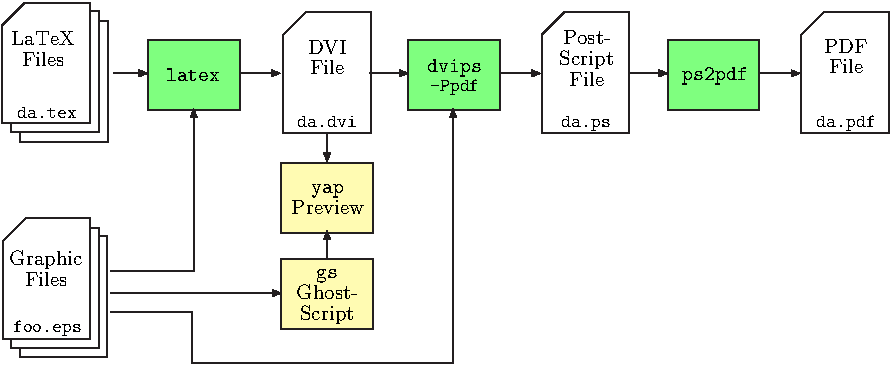
\includegraphics[width=1.0\textwidth]{workflow-cm}
\caption{Erzeugung von
PDF-Doku\-men\-ten im DVI-PS-Workflow. EPS-Grafiken werden erst bei der
Erzeugung der PS-Datei eingebunden. 
Anmerkung: Die abgebildete Vektorgrafik wurde mit \emph{Freehand} unter
Verwendung der \emph{BaKoMa} TrueType-Schriften erstellt %
(s.\ Abschn.\ \ref{sec:tex-schriften-in-grafiken}).}
\label{fig:latex-pdf-workflow}
\end{figure}

\end{comment}


\section{Drucken}

Vor dem Drucken der Arbeit empfiehlt es sich, einige Dinge zu beachten, um unnötigen Aufwand (und auch Kosten) zu vermeiden.

\subsection{Drucker und Papier}

Die Abschlussarbeit sollte in der Endfassung unbedingt auf einem
qualitativ hochwertigen Laserdrucker ausgedruckt werden, Ausdrucke
mit Tintenstrahldruckern sind \emph{nicht} ausreichend. Auch das
verwendete Papier sollte von guter Qualität (holzfrei) und
üblicher Stärke (mind.\ $80\; {\mathrm g} / {\mathrm m}^2$) sein.
Falls \emph{farbige} Seiten notwendig sind, sollte man diese einzeln%
\footnote{Tip: Mit \emph{Adobe Acrobat} lassen sich sehr einfach einzelne Seiten
des Dokuments für den Farbdruck auswählen und zusammenstellen.}
auf einem Farb-Laserdrucker ausdrucken und dem Dokument beifügen.

Übrigens sollten \emph{alle} abzugebenden Exemplare \textbf{gedruckt} (und nicht kopiert) werden! Die Kosten für den Druck
sind heute nicht höher als die für Kopien, der
Qualitätsunterschied ist jedoch -- \va\ bei Bildern und Grafiken
-- meist deutlich.


\subsection{Druckgröße}

Zunächst sollte sichergestellt werden, dass die in der fertigen PDF-Datei eingestellte
Papiergröße tatsächlich \textbf{A4} ist! Das geht \zB\ mit \emph{Adobe Acrobat}
oder \emph{SumatraPDF}
über \texttt{File} $\rightarrow$ \texttt{Properties},
wo die Papiergröße des Dokuments angezeigt wird:
\begin{center}
\textbf{Richtig:} A4 = $8{,}27 \times 11{,}69$ in \bzw\ $21{,}0 \times 29{,}7$ cm.
\end{center}
Falls das nicht stimmt, ist vermutlich irgendwo im Workflow versehentlich \textbf{Letter} 
als Papierformat eingestellt, %, häufig ist \emph{Adobe Distiller} "schuld".


Ein häufiger und leicht zu übersehender Fehler beim Ausdrucken von
PDF-Doku\-menten wird durch die versehentliche Einstellung der
Option "Fit to page" im Druckmenü verursacht, wobei die Seiten
meist zu klein ausgedruckt werden. Überprüfen Sie daher die Größe
des Ausdrucks anhand der eingestellten Zeilenlänge oder mithilfe
einer Messgrafik, wie am Ende dieses Dokuments gezeigt.
Sicherheitshalber sollte diese Messgrafik bis zur
Fertigstellung der Arbeit beibehalten und die entsprechende
Seite erst ganz am Schluss zu entfernt werden.
Wenn, wie häufig der Fall, einzelne Seiten getrennt in Farbe gedruckt 
werden, so sollten natürlich auch diese genau auf die Einhaltung der Druckgröße 
kontrolliert werden!




\section{Binden}

Die Endfassung der Abschlussarbeit%
\footnote{Für \textbf{Bachelorarbeiten} genügt, je nach Vorgaben des Studiengangs, meist eine einfache Bindung (Copyshop oder Bibliothek).}
ist in fest gebundener Form
einzureichen.%
\footnote{An der Fakultät Hagenberg ist bei Masterarbeiten zumindest eines der
Exemplare \emph{ungebunden} abzugeben -- dieses wird später von einem
Buchbinder in einheitlicher Form gebunden und verbleibt
danach in der Bibliothek. Datenträger sind bei diesem Exemplar lose 
und \emph{ohne} Aufkleber (jedoch beschriftet) beizulegen.}
Dabei ist eine Bindung zu
verwenden, die das Ausfallen von einzelnen Seiten nachhaltig
verhindert, \zB durch eine traditionelle Rückenbindung
(Buchbinder) oder durch handelsübliche Klammerungen aus Kunststoff
oder Metall. Eine einfache Leimbindung ohne Verstärkung ist
jedenfalls \emph{nicht} ausreichend.


Falls man -- was sehr zu empfehlen ist -- die Arbeit bei einem
professionellen Buchbinder durchführen lässt, sollte man auch auf
die Prägung am Buchrücken achten, die kaum zusätzliche Kosten
verursacht. Üblich ist dabei die Angabe des Familiennamens des
Autors und des Titels der Arbeit. Ist der Titel der Arbeit zu
lang, muss man notfalls eine gekürzte  Version angeben, wie \zB:
%
\begin{center}
\setlength{\fboxsep}{3mm}
\fbox{
\textsc{Schlaumeier}
\textperiodcentered\ \textsc{Part.\ Lösungen zur allg.\ Problematik}}
\end{center}
%



\section{Elektronische Datenträger (CD-R, DVD, USB-Stick)}
Speziell bei Arbeiten im Bereich der Informationstechnik (aber
nicht nur dort) fallen fast immer Informationen an, wie Programme,
Daten, Grafiken, Kopien von Internetseiten \usw, die für eine
spätere Verwendung elektronisch verfügbar sein sollten.
Vernünftigerweise wird man diese Daten während der Arbeit bereits
gezielt sammeln und der fertigen Arbeit auf einer CD-ROM, DVD oder
einem USB-Stick beilegen. Es ist außerdem sinnvoll -- schon allein
aus Gründen der elektronischen Archivierbarkeit -- die eigene Arbeit
selbst als PDF-Datei beizulegen.%
\footnote{Auch Bilder und Grafiken könnten in elektronischer Form nützlich
sein, die \latex- oder Word-Dateien sind hingegen überflüssig.}


Falls ein elektronischer Datenträger (CD-ROM, DVD, USB-Stick) beigelegt
wird, sollte auf folgende Dinge geachtet werden:
%
\begin{enumerate}
\item Jedem abzugebenden Exemplar muss eine identische Kopie des
Datenträgers beiliegen. %
\item Verwenden Sie qualitativ hochwertige Rohlinge und überprüfen
Sie nach der Fertigstellung die tatsächlich gespeicherten Inhalte
des Datenträgers! %
\item Der Datenträger sollte in eine im hinteren Umschlag
eingeklebte Hülle eingefügt sein und sollte so zu entnehmen sein,
dass die Hülle dabei \emph{nicht} zerstört wird (die
meisten Buchbinder haben geeignete Hüllen parat). %
\item Der Datenträger muss so beschriftet sein, dass er der
Abschlussarbeit eindeutig zuzuordnen ist, am Besten durch ein
gedrucktes Label%
\footnote{Nicht beim lose abgegebenen Bibliotheksexemplar --
dieses erhält ein standardisiertes Label durch die Bibliothek.} %
oder sonst durch \emph{saubere}
Beschriftung mit
der Hand und einem feinen, wasserfesten Stift. %
\item Nützlich ist auch ein (grobes) Verzeichnis der Inhalte des
Datenträgers (wie exemplarisch in Anhang \ref{app:cdrom}).
\end{enumerate}

\chapter{Schlussbemerkungen}
\label{cha:Schluss}



%%%----------------------------------------------------------
\appendix                                            % Anhang 
%%%----------------------------------------------------------

\chapter{Technische Informationen}
\label{app:TechnischeInfos}

	% Technische Ergänzungen
\chapter{Inhalt der CD-ROM/DVD}
\label{app:cdrom}

	% Inhalt der CD-ROM/DVD
\chapter{Fragebogen}
\label{app:Fragebogen}

	% Chronologische Liste der Änderungen
\chapter{\latex-Quellkode}
\label{app:Quellcode}

	% Quelltext dieses Dokuments

%%%----------------------------------------------------------
\MakeBibliography                        % Quellenverzeichnis
%%%----------------------------------------------------------

%%% Messbox zur Druckkontrolle ------------------------------
\chapter*{Messbox zur Druckkontrolle}



\begin{center}
{\Large --- Druckgröße kontrollieren! ---}

\bigskip

\calibrationbox{100}{50} % Angabe der Breite/Hoehe in mm

\bigskip

{\Large --- Diese Seite nach dem Druck entfernen! ---}

\end{center}



%%%----------------------------------------------------------
\end{document}
%%%----------------------------------------------------------| returns and the picture is ready. From this point on, the
external graphics will be used.

There is another possibility to communicate \meta{main document} to the
subprocess performing the externalization: namely to write
`|\tikzexternalize{main}|' into the document. In this case, the conversion
system call will be
%
\begin{codeexample}[code only, tikz syntax=false]
pdflatex -jobname "main-figure0" "main"
\end{codeexample}
%
\noindent and the contents of |\tikzexternalrealjob| is set automatically. This
case is detected by |\tikzexternalize|, and the |system call| is updated
automatically (by patching its |\texsource| template argument). It is not
necessary to change the |system call| manually.

The sequence in which system calls are performed and the decision whether they
are issued automatically is governed by the |mode| key, consult its
documentation for details.


\subsection{Using External Graphics Without \textmd{\pgfname}\ Installed}
\label{section-libs-external-nopgf}

Given that every picture has been exported correctly, one may want to compile a
file without \pgfname\ and \tikzname\ installed. \tikzname\ comes with a
minimal package which contains just enough commands to replace every
|tikzpicture| environment and the |\tikz| short command with the appropriate
external graphics. It can be found at
%
\begin{codeexample}[code only, tikz syntax=false]
latex/pgf/utilities/tikzexternal.sty
\end{codeexample}
%
\noindent and needs to be used instead of |\usepackage{tikz}|. So, we uncomment
|\usepackage{tikz}| and our example from the beginning becomes
%
\begin{codeexample}[code only]
\documentclass{article}
% main document, called main.tex
%\usepackage{tikz}

\usepackage{graphicx}
\usepackage{tikzexternal}

%\usetikzlibrary{external}
\tikzexternalize

\begin{document}
\begin{tikzpicture}
  \node {root}
    child {node {left}}
    child {node {right}
      child {node {child}}
      child {node {child}}
    };
\end{tikzpicture}

A simple image is \tikz \fill (0,0) circle(5pt);.

Furthermore, we might want to draw \tikz[baseline]\draw (0,-1) rectangle (1,1);
\end{document}
\end{codeexample}
%
\noindent where the following files are necessary to compile the document:
%
\begin{codeexample}[code only, tikz syntax=false]
tikzexternal.sty
main.tex
main-figure0.pdf
main-figure1.pdf
main-figure2.pdf
\end{codeexample}
%
\noindent If there are any `|.dpth|' files, for example |main-figure2.dpth|,
these files are also required. They contain information for the \tikzname\
|baseline| option (or |\label|s inside external graphics).

Just copy the |.sty| file into the directory of your |main.tex| file and use it
as part of your document.

Please keep in mind, that only |tikzpicture| environments and |\tikz| short
images are available within the externalization framework. Additionally, calls
to |\tikzset| and |\pgfkeys| won't lead to compilation errors because they are
simply ignored. But since |pgfkeys| is not available, any option supplied to
|\tikzexternalize| is \emph{ignored}.

\paragraph{Attention:}
Since the simple replacement |\usepackage{tikzexternal}| doesn't support the
key--value interface, you \emph{need} to use |\tikzsetexternalprefix| instead
of the |prefix| option and |\tikzsetfigurename| instead of the |figure name|
option since |\tikzset| is not available in such a context.

\paragraph{Remark:}
Some of the features of this library are mainly useful to improve the speed of
successive document compilations. In other words: you can't use all features in
this context, keep it simple.


\subsection{\texttt{eps} Graphics Export}

It is also possible to use \eps\ graphics instead of \pdf\ files. There are
different ways to produce them, for example to use |pdflatex| and call
|pdftops -eps |\marg{pdf file} \marg{eps file} afterwards. You could add this
command to the |system call| option.

Alternatively, you can use |latex| and |dvips| for image conversion as is
explained for the |system call| option, see
page~\pageref{extlib:systemcall:option}. See the documentation for the basic
level externalization in section~\ref{section-external} for restrictions of
other drivers.


\subsection{Bitmap Graphics Export}

Occasionally, you may have an extremely large graphics which takes long times
to render. It might be interesting to generate a bitmap (raster) image, which
displays much faster (for example in a presentation). I have used this feature
to speed-up the display of large shadings.

The |external| library can be customized to export bitmap images -- with the
help of external programs. Due to the dependence of external programs, you may
need to adjust these commands manually. For example, on my computer, the
ImageMagick Suite is installed which comes with the |convert| tool. Together
with |pdflatex|, I can define the following style:
%
\begin{codeexample}[code only]
\tikzset{
    % Defines a custom style which generates BOTH, .pdf and .png export
    % but prefers the .png on inclusion.
    %
    % This style is not pre-defined, you may need to copy-paste and
    % adjust it.
    png export/.style={
        external/system call/.add=
            {}
            {; convert -density 300 -transparent white "\image.pdf" "\image.png"},
        %
        /pgf/images/external info,
        /pgf/images/include external/.code={%
            \includegraphics
                [width=\pgfexternalwidth,height=\pgfexternalheight]
                {##1.png}%
        },
    }
}
\end{codeexample}
%
\noindent The example above defines a new style called `|png export|' which,
when it is set with |\tikzset{png export}| somewhere in the document, modifies
the configuration for both file generation and file input. The file generation
is modified by appending the ImageMagick command to |system call| (separated by
`|;|' as usual on Linux). This is, in principle, enough to generate a |.png|
file. The |include external| command is overwritten such that it uses the
|.png| file instead of the |.pdf| file (which exists as well in the
configuration above). But since a |.png| file can have a much higher resolution
than the desired image dimensions, we have to add |width| and |height|
explicitly. Usually, the |external| library does not provide size information
(it is unnecessary for |.pdf| or |.eps| since these formats have their bounding
box information). To enable size information, the style uses the
|external info| key, which, in turn, provides the |\pgfexternalwidth| and
|\pgfexternalheight| commands.

Now we can use |\tikzset{png export}| either document-wide or just for one
particular image. The configuration remains in effect until the end of the
current environment (or until the next closing curly brace `|}|').

\begin{key}{/pgf/images/external info=\marg{boolean} (initially false)}
    If this key is activated, the size for any externalized image will be
    stored explicitly into the associated |.dpth| file.

    When the file is included by |\pgfincludeexternalgraphics| (or
    automatically by the |external| library), the width is available as
    \declareandlabel{\pgfexternalwidth} and the height as
    \declareandlabel{\pgfexternalheight}.
\end{key}


\subsection{Compatibility Issues}

\subsubsection{References In External Pictures}

It is allowed if a picture contains references, for example
|\tikz \node {Reference to \ref{a:label}};|.

There is just one issue: if the main job is currently compiling, its |.aux|
file is not in its final state (even worse: it may not be readable at all). The
picture externalization, however, needs the main |.aux| file to query any
references.

Thus, you \emph{will} need to invoke
|pdflatex -jobname |\meta{image}| |\meta{mainfile} \emph{manually}
for any image which contains references.

This problem arises only for |mode=convert with system call|. In this case,
the |external| library creates a special |\jobname.auxlock| file to check
whether the main |.aux| file is currently usable.


\subsubsection{Compatibility With Other Libraries or Packages}

The |external| library has the following compatibility issues:
%
\begin{enumerate}
    \item The |external| library comes with special support for
        |\usetikzlibrary{fadings}|: the |fadings| library may define local
        pictures which would be externalized (although they shouldn't). There
        is special handling to suppress this bug if |\tikzexternalize| is
        called \emph{after} |\usetikzlibrary{fadings}| or if all fadings are
        defined \emph{before} |\tikzexternalize|.
    \item Problems have been reported when using |\tikzexternalize| (or the
        basic layer externalization) together with |\usepackage{glossary}|.
        This problem disappears if |\tikzexternalize| is called \emph{before}
        |\usepackage{glossary}|.
    \item Problems with |\usepackage{pdfpages}| and |\usepackage{vmargin}|: The
        |external| library replaces the current shipout routine of \TeX\ during
        its externalization. This might raise problems with other packages
        which also manipulate the shipout routine (like the mentioned ones). To
        fix those problems, use
        %
\begin{codeexample}[code only]

\usetikzlibrary{external}

\tikzifexternalizing{%
    % don't include package XYZ here
}{%
    \usepackage{pdfpages}
    \usepackage{vmargin}
    ...
}%
\end{codeexample}
        %
        This uses the requested packages for the main document, but not for the
        single, exported graphics.
\end{enumerate}

In general, the |\tikzifexternalizing| feature might be used to solve package
conflicts and the |\tikzexternaldisable| and |\tikzexternalenable| features can
be used to solve problems with single pictures.


\subsubsection{Compatibility With Bounding Box Restrictions}

Bounding box restrictions provide no problem when used with \eps\ graphics.
However, they pose problems for |pdflatex|, so you may need to use the
|latex|/|dvips| combination if you use bounding box restrictions and
externalization. Currently, the only possibility for bounding box restrictions
and |pdflatex| is to use a combination of |trim left|/|trim right|/|baseline|:
these keys do not \emph{really} truncate the bounding box, they only store
horizontal and vertical shifts (also see the |trim lowlevel| key in this
context).


\subsubsection{Interoperability With The Basic Layer Externalization}

This library is fully compatible with
|\beginpgfgraphicnamed|$\dotsc$|\endpgfgraphicnamed| environments. However, you
will need to use the |export next=false| key to avoid conflicts:
%
\begin{codeexample}[code only]
\beginpgfgraphicnamed{picture4}
\tikzset{external/export next=false}
\begin{tikzpicture}
   \draw (0,0) -- (4,4);
\end{tikzpicture}
\endpgfgraphicnamed
\end{codeexample}
%
Please keep in mind that file prefixes do not apply to the basic layer.
}
